% !TEX root = ../Elements.tex
%%%%%%
% BOOK 13
%%%%%%
\pdfbookmark[0]{Book 13}{book13}
\pagestyle{empty}
\begin{center}
{\Huge ELEMENTS BOOK 13}\\
\spa\spa\spa
{\huge\it The Platonic Solids\symbolfootnote[2]{The five regular solids---the cube, tetrahedron ({\rm i.e.}, pyramid), octahedron, icosahedron, and dodecahedron---were problably discovered by the school of Pythagoras. They are generally termed ``Platonic'' solids because they feature prominently in Plato's famous dialogue {\em Timaeus}. Many of the theorems contained in this book---particularly those which pertain to the last two solids---are ascribed to Theaetetus of Athens.}}
\end{center}
\vspace{2cm}
% Removed epsf size command
\centerline{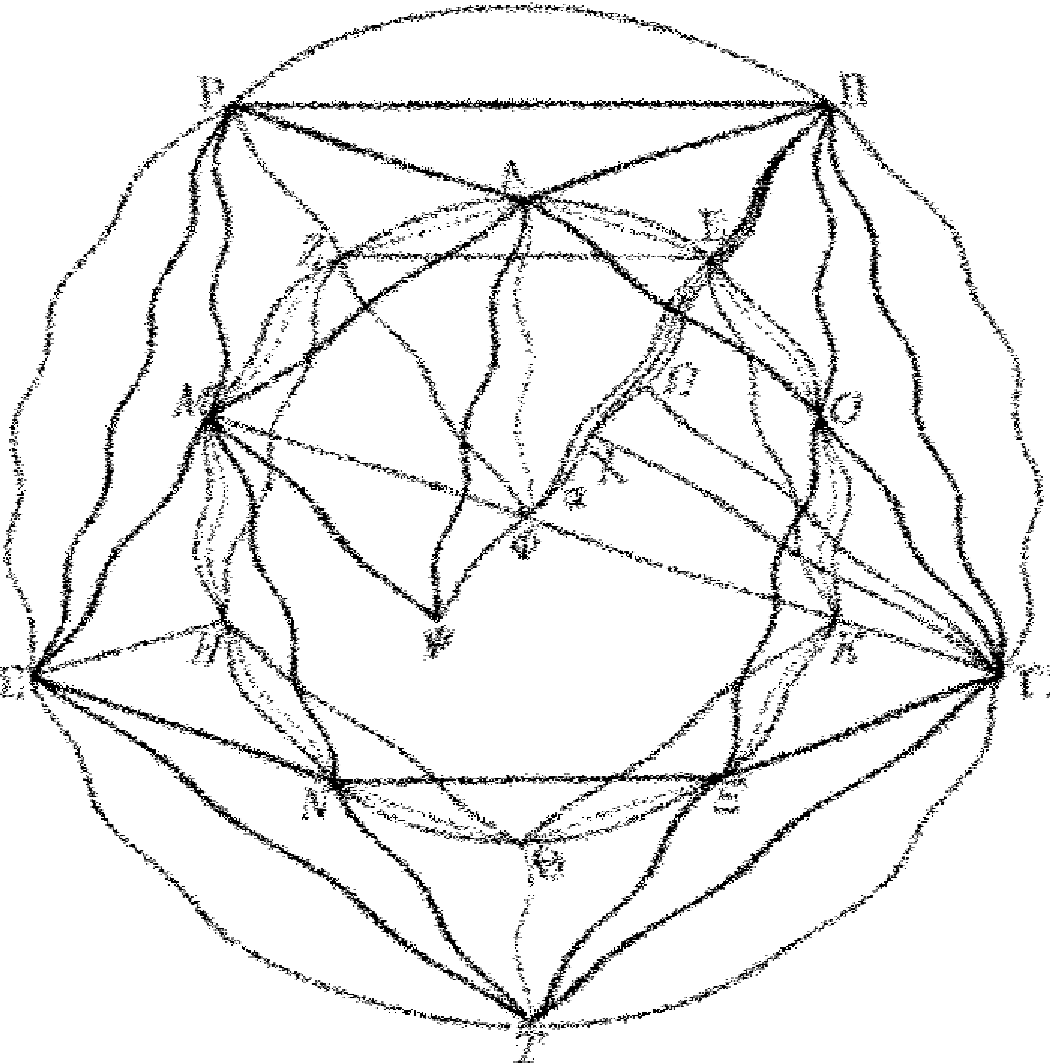
\includegraphics{Book13/front.pdf}}
\newpage

%%%%
%13.1
%%%%
\pdfbookmark[1]{Proposition 13.1}{pdf13.1}
\pagestyle{fancy}
\cfoot{\gr{\kern -.7pt }}
\lhead{\large\gr{ΣΤΟΙΘΕΙΩΝ \kern -.7pt {13}.}}
\rhead{\large ELEMENTS BOOK 13}
\begin{Parallel}{}{}
\ParallelLText{
\begin{center}
{\large \ggn{1}.}
\end{center}\vspace*{-7pt}

\gr{Ἐὰν εὐθεῖα γραμμ\kern -.7pt  ὴ >άκρον καὶ μέσον λόγον τμ\kern -.7pt  ηθῆ|, τὸ
μεῖζον τμ\kern -.5pt  ῆμα προσλαβὸν τὴν ἡμίσειαν τῆξ <όληξ πενταπλάσιον
δύναται τοῦ ἀπὸ τῆξ ἡμισείαξ τετραγώνου.}

% Removed epsf size command
\centerline{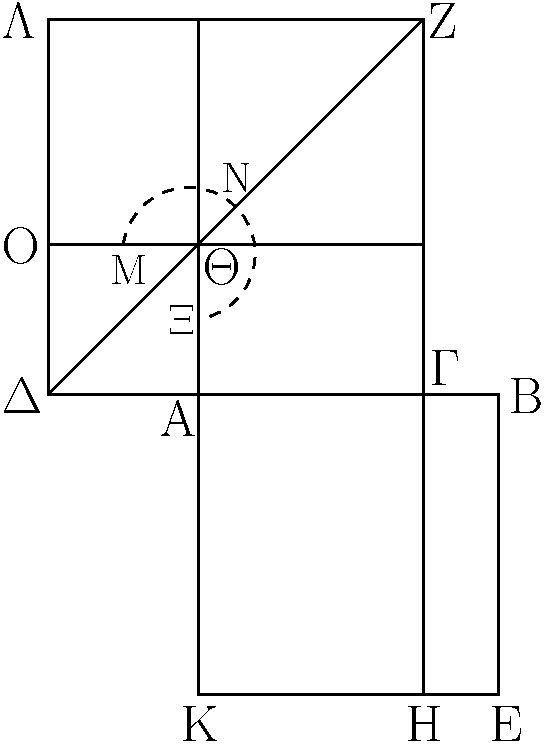
\includegraphics{Book13/fig01g.pdf}}

\gr{Εὐθεῖα γὰρ γραμμ\kern -.7pt  ὴ ἡ ΑΒ >άκρον καὶ μέσον λόγον τετμ\kern -.7pt  ήσθω
κατὰ τὸ Γ σημεῖον, καὶ >έστω μεῖζον τμ\kern -.5pt  ῆμα τὸ ΑΓ, καὶ
ἐκβεβλήσθω ἐπ> εὐθείαξ τῆ| ΓΑ εὐθεῖα ἡ ΑΔ, καὶ κείσθω
τῆξ ΑΒ ἡμίσεια ἡ ΑΔ; λέγω, <ότι πενταπλάσιόν ἐστι τὸ ἀπὸ
τῆξ ΓΔ τοῦ ἀπὸ τῆξ ΔΑ.}

\gr{Ἀναγεγράφθωσαν γὰρ ἀπὸ τῶν ΑΒ, ΔΓ τετράγωνα τὰ ΑΕ,
ΔΖ, καὶ καταγεγράφθω ἐν τῶ| ΔΖ τὸ σθῆμα, καὶ διήθθω ἡ ΖΓ
ἐπὶ τὸ Η. καὶ ἐπεὶ ἡ ΑΒ >άκρον καὶ μέσον λόγον τέτμ\kern -.7pt  ηται
κατὰ τὸ Γ, τὸ >άρα ὑπὸ τῶν ΑΒΓ >ίσον ἐστὶ τῶ| ἀπὸ τῆξ
ΑΓ. καί ἐστι τὸ μὲν ὑπὸ τῶν ΑΒΓ τὸ ΓΕ, τὸ δὲ ἀπὸ τῆξ
ΑΓ τὸ ΖΘ; >ίσον >άρα τὸ ΓΕ τῶ| ΖΘ. καὶ ἐπεὶ διπλῆ ἐστιν
ἡ ΒΑ τῆξ ΑΔ, >ίση δὲ ἡ μὲν ΒΑ τῆ| ΚΑ, ἡ δὲ ΑΔ τῆ|
ΑΘ, διπλῆ >άρα καὶ ἡ ΚΑ τῆξ ΑΘ. ὡξ δὲ ἡ ΚΑ πρὸξ τὴν
ΑΘ, ο<ύτωξ τὸ ΓΚ πρὸξ τὸ ΓΘ;
διπλάσιον >άρα τὸ ΓΚ τοῦ ΓΘ. εἰσὶ δὲ καὶ τὰ ΛΘ, ΘΓ διπλάσια
τοῦ ΓΘ. >ίσον >άρα τὸ ΚΓ τοῖξ ΛΘ, ΘΓ. ἐδείθθη δὲ καὶ τὸ ΓΕ
τῶ| ΘΖ >ίσον; <όλον >άρα τὸ ΑΕ τετράγωνον >ίσον ἐστὶ τῶ|
ΜΝΧ γνώμονι. καὶ ἐπεὶ διπλῆ ἐστιν ἡ ΒΑ τῆξ ΑΔ,
τετραπλάσιόν ἐστι τὸ ἀπὸ τῆξ ΒΑ τοῦ ἀπὸ τῆξ ΑΔ, τουτέστι
τὸ ΑΕ τοῦ ΔΘ. >ίσον δὲ τὸ ΑΕ τῶ| ΜΝΧ γνώμονι; καὶ ὁ
ΜΝΧ >άρα γνώμων τετραπλάσιόξ ἐστι τοῦ ΑΟ; <όλον >άρα
τὸ ΔΖ πενταπλάσιόν ἐστι τοῦ ΑΟ. καί ἐστι τὸ μὲν ΔΖ τὸ
ἀπὸ τῆξ ΔΓ, τὸ δὲ ΑΟ τὸ ἀπὸ τῆξ ΔΑ; τὸ >άρα ἀπὸ
τῆξ ΓΔ πενταπλάσιόν ἐστι τοῦ ἀπὸ τῆξ ΔΑ.}

\gr{Ἐὰν >άρα εὐθεῖα >άκρον καὶ μέσον λόγον τμ\kern -.7pt  ηθῆ|,
τὸ μεῖζον τμ\kern -.7pt  ῆμα προσλαβὸν τὴν ἡμίσειαν τῆξ <όληξ
πενταπλάσιον δύναται τοῦ ἀπὸ τῆξ ἡμισείαξ τετραγώνου;
<όπερ >έδει δεῖχαι.}}

\ParallelRText{
\begin{center}
{\large Proposition 1}
\end{center}

If a straight-line is cut in extreme and mean ratio then the square on the
greater piece, added to half of the whole, is  five times the square
on the half.

% Removed epsf size command
\centerline{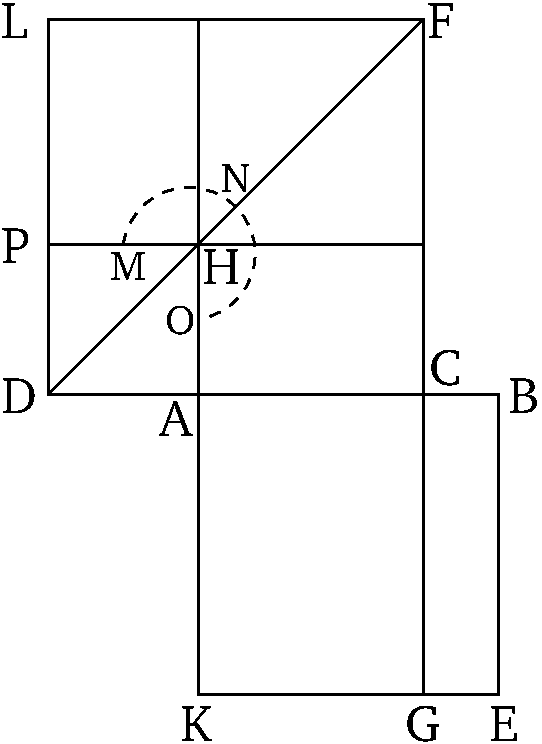
\includegraphics{Book13/fig01e.pdf}}

For let the straight-line $AB$ be cut in extreme and mean ratio at
point $C$, and let $AC$ be the greater piece. And let the straight-line
$AD$ be produced in a straight-line with $CA$. And let
$AD$ be made (equal to) half of $AB$. I say that the (square) on
$CD$ is five times the (square) on $DA$. 

For let the squares $AE$ and $DF$ be described on $AB$ and
$DC$ (respectively). And let the figure in $DF$ be drawn.  
And let $FC$ be drawn across to $G$. And since $AB$ has been
cut in extreme and mean ratio at $C$, the (rectangle
contained) by $ABC$ is thus equal to the (square) on $AC$ [Def.~6.3, Prop.~6.17].
And  $CE$ is the (rectangle contained) by $ABC$, and $FH$ the
(square) on $AC$. Thus, $CE$ (is) equal to $FH$. 
And since $BA$ is double $AD$, and $BA$ (is) equal to $KA$,
and $AD$ to $AH$, $KA$ (is) thus also double $AH$. 
And as $KA$ (is) to $AH$, so $CK$ (is) to $CH$ [Prop.~6.1].
Thus, $CK$ (is) double $CH$. And $LH$ plus $HC$ is also double $CH$
[Prop.~1.43].  Thus, $KC$ (is) equal to $LH$ plus $HC$. And
$CE$ was also shown (to be) equal to $HF$. Thus, the whole square
$AE$ is equal to the gnomon $MNO$. And since $BA$ is double
$AD$, the (square) on $BA$ is four times the (square) on $AD$---that
is to say, $AE$ (is four times) $DH$. And $AE$ (is) equal to
gnomon $MNO$. And, thus, gnomon $MNO$ is also four times $AP$. 
Thus, the whole of $DF$ is five times $AP$. And $DF$ is the (square)
on $DC$, and $AP$ the (square) on $DA$. Thus, the
(square) on $CD$ is five times the (square) on $DA$. 

Thus, if a straight-line is cut in extreme and mean ratio then the square on the
greater piece, added to half of the whole, is five times the square
on the half. (Which is) the very thing it was required to show.\\}
\end{Parallel}

%%%%
%13.2
%%%%
\pdfbookmark[1]{Proposition 13.2}{pdf13.2}
\begin{Parallel}{}{}
\ParallelLText{
\begin{center}
{\large \ggn{2}.}
\end{center}\vspace*{-7pt}

\gr{Ἐὰν εὐθεῖα γραμμ\kern -.7pt  ὴ τμ\kern -.7pt  ήματοξ ἑαυτῆξ πενταπλάσιον δύνηται,
τῆξ διπλασίαξ τοῦ εἰρημένου τμ\kern -.5pt  ήματοξ >άκρον καὶ μέσον
λόγον τεμνομένηξ τὸ μεῖζον τμ\kern -.3pt  ῆμα τὸ λοιπὸν μέροξ ἐστὶ
τῆξ ἐχ ἀρθῆξ εὐθείαξ.}

% Removed epsf size command
\centerline{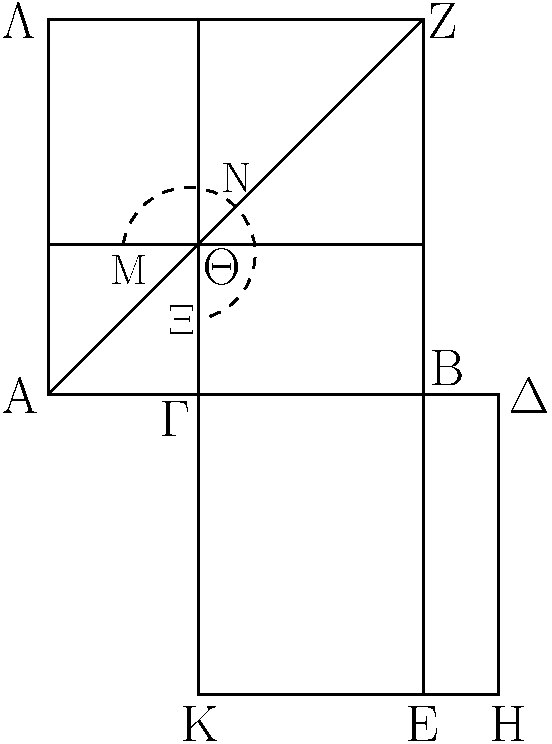
\includegraphics{Book13/fig02g.pdf}}

\gr{Εὐθεῖα γὰρ γραμμ\kern -.7pt  ὴ ἡ ΑΒ τμ\kern -.7pt  ήματοξ ἑαυτῆξ τοῦ ΑΓ
πενταπλάσιον δυνάσθω, τῆξ δὲ ΑΓ διπλῆ >έστω ἡ ΓΔ. λέγω,
<ότι τῆξ ΓΔ >άκρον καὶ μέσον λόγον τεμνομένοξ τὸ μεῖζον
τμ\kern -.5pt  ῆμά ἐστιν ἡ ΓΒ.}

\gr{Ἀναγεγράφθω γὰρ ἀφ> ἑκατέραξ τῶν ΑΒ, ΓΔ τετράγωνα
τὰ ΑΖ, ΓΗ, καὶ καταγεγράφθω ἐν τῶ| ΑΖ τὸ σθῆμα, καὶ διήθθω
ἡ ΒΕ. καὶ ἐπεὶ πενταπλάσιόν ἐστι τὸ ἀπό τῆξ ΒΑ τοῦ ἀπὸ
τῆξ ΑΓ, πενταπλάσιόν ἐστι τὸ ΑΖ τοῦ ΑΘ. τετραπλάσιοξ
>άρα ὁ ΜΝΧ γνώμων τοῦ ΑΘ. καὶ ἐπεὶ διπλῆ ἐστιν ἡ ΔΓ
τῆξ ΓΑ, τετραπλάσιον >άρα ἐστὶ τὸ ἀπὸ ΔΓ τοῦ ἀπὸ ΓΑ,
τουτέστι τὸ ΓΗ τοῦ ΑΘ. ἐδείθθη δὲ καὶ ὁ ΜΝΧ
γνώμων τετραπλάσιοξ τοῦ ΑΘ; >ίσοξ >άρα ὁ ΜΝΧ γνώμων
τῶ| ΓΗ. καὶ ἐπεὶ διπλῆ ἐστιν ἡ ΔΓ τῆξ ΓΑ, >ίση δὲ ἡ
μὲν ΔΓ τῆ| ΓΚ, ἡ δὲ ΑΓ τῆ| ΓΘ, [διπλῆ >άρα καὶ ἡ ΚΓ τῆξ ΓΘ], διπλάσιον >άρα καὶ τὸ ΚΒ τοῦ ΒΘ. εἰσὶ δὲ καὶ
τὰ ΛΘ, ΘΒ τοῦ ΘΒ διπλάσια; >ίσον >άρα τὸ ΚΒ τοῖξ ΛΘ, ΘΒ.
ἐδείθθη δὲ καὶ <όλοξ ὁ ΜΝΧ γνώμων <όλῳ τῶ| ΓΗ >ίσοξ;
καὶ λοιπὸν >άρα τὸ ΘΖ τῶ| ΒΗ ἐστιν >ίσον. καί ἐστι τὸ μὲν
ΒΗ τὸ ὑπὸ τῶν ΓΔΒ; >ίση γὰρ ἡ ΓΔ τῆ| ΔΗ; τὸ δὲ ΘΖ
τὸ ἀπὸ τῆξ ΓΒ; τὸ >άρα ὑπὸ τῶν ΓΔΒ >ίσον ἐστὶ τῶ|
ἀπὸ τῆξ ΓΒ. >έστιν >άρα ὡξ ἡ ΔΓ πρὸξ τὴν ΓΒ, ο<ύτωξ
ἡ ΓΒ πρὸξ τὴν ΒΔ. μείζων δὲ ἡ ΔΓ τῆξ ΓΒ; μείζων >άρα καὶ
ἡ ΓΒ τῆξ ΒΔ. τῆξ ΓΔ >άρα εὐθείαξ >άκρον καὶ μέσον λόγον
τεμνομένηξ τὸ μεῖζον τμ\kern -.7pt  ῆμά ἐστιν ἡ ΓΒ.}

\gr{Ἐὰν >άρα εὐθεῖα γραμμ\kern -.7pt  ὴ τμ\kern -.7pt  ήματοξ ἑαυτῆξ πενταπλάσιον
δύνηται, τῆξ διπλασίαξ τοῦ εἰρημένου τμ\kern -.5pt  ήμ\-ατοξ >άκρον καὶ
μέσον λόγον τεμνομένηξ τὸ μεῖζον τμ\kern -.3pt  ῆμα τὸ λοιπὸν μέροξ
ἐστὶ τῆξ ἐχ ἀρθῆξ εὐθείαξ; <όπερ >έδει δεῖχαι.}}

\ParallelRText{
\begin{center}
{\large Proposition 2}
\end{center}

If the square on a straight-line is five times the (square) on a piece of
it, and  double the aforementioned piece is cut in extreme and
mean ratio, then the greater piece  is  the remaining part of the
original straight-line. 

% Removed epsf size command
\centerline{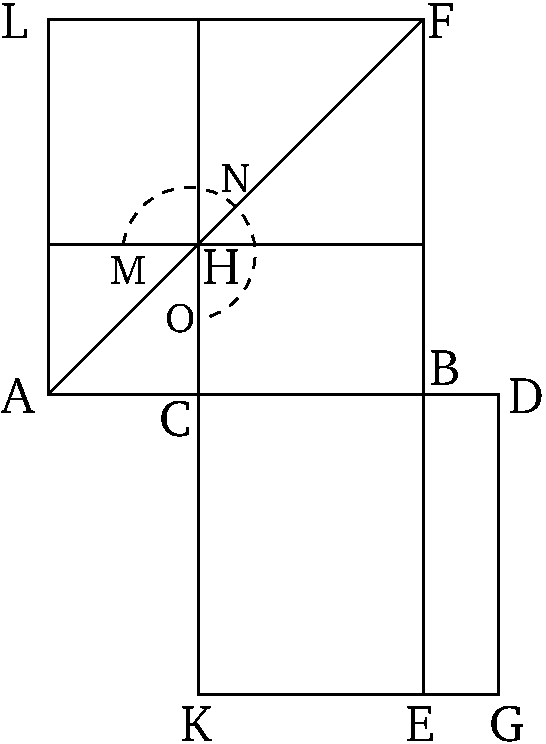
\includegraphics{Book13/fig02e.pdf}}

For let the square on the straight-line $AB$ be five times the (square)
on the piece of it, $AC$. And let $CD$ be double $AC$. I say that
if $CD$ is cut in extreme and mean ratio then the greater piece
is $CB$. 

For let the squares $AF$ and $CG$ be described on each of
$AB$ and $CD$ (respectively). And let the figure  in $AF$ be drawn.
And let $BE$ be drawn across. And since the (square) on $BA$
is five times the (square) on $AC$, $AF$ is five times $AH$. 
Thus, gnomon $MNO$ (is) four times $AH$. 
And since
$DC$ is double $CA$, the (square) on $DC$ is thus four times the (square)
on $CA$---that is to say, $CG$ (is four times) $AH$. And the gnomon
$MNO$ was also shown (to be) four times $AH$. Thus, gnomon $MNO$
(is) equal to $CG$. And since $DC$ is double $CA$, and $DC$
(is) equal to $CK$, and $AC$ to $CH$, [$KC$ (is) thus also double $CH$], (and) $KB$ (is) also double $BH$
[Prop.~6.1]. And $LH$ plus $HB$ is also double $HB$ [Prop.~1.43].
Thus, $KB$ (is) equal to $LH$ plus $HB$. And the whole gnomon
$MNO$ was also shown (to be) equal to the whole of $CG$. Thus, the
remainder $HF$ is also equal to (the remainder) $BG$.  And $BG$
is the (rectangle contained) by $CDB$. For  $CD$ (is) equal to $DG$.
And $HF$ (is) the square on $CB$. Thus, the (rectangle contained)
by $CDB$ is equal to the (square) on $CB$. Thus, as $DC$ is to $CB$,
so $CB$ (is) to $BD$ [Prop.~6.17]. And $DC$ (is) greater than $CB$ (see lemma). Thus, $CB$ (is) also greater than $BD$ [Prop.~5.14]. Thus, if the
straight-line $CD$ is cut in extreme and mean ratio then the greater piece is $CB$.

Thus, if the square on a straight-line is five times the (square) on a piece of
itself, and  double the aforementioned piece is cut in extreme and
mean ratio, then the greater piece is the remaining part of the
original straight-line.  (Which is) the very thing it was required to show.}
\end{Parallel}

\begin{Parallel}{}{}
\ParallelLText{
\begin{center}
{\large \gr{Λῆμμα}.}
\end{center}\vspace*{-7pt}

\gr{<'Οτι δὲ ἡ διπλῆ τῆξ ΑΓ μείζων ἐστὶ τῆξ ΒΓ, ο<ύτωξ
δεικτέον.}

\gr{Εἰ γὰρ μ\kern -.7pt  ή, >έστω, εἰ δυνατόν, ἡ ΒΓ διπλῆ τῆξ ΓΑ.
τετραπλάσιον >άρα τὸ ἀπὸ τῆξ ΒΓ τοῦ ἀπὸ τῆξ ΓΑ;
πενταπλάσια >άρα τὰ ἀπὸ τῶν ΒΓ, ΓΑ τοῦ ἀπὸ
τῆξ ΓΑ. ὑπόκειται δὲ καὶ τὸ ἀπὸ τῆξ ΒΑ πενταπλάσιον
τοῦ ἀπὸ τῆξ ΓΑ; τὸ >άρα ἀπὸ τῆξ ΒΑ >ίσον ἐστὶ
τοῖξ ἀπὸ τῶν ΒΓ, ΓΑ; <όπερ ἀδύνατον. οὐκ >άρα
ἡ ΓΒ διπλασία ἐστὶ τῆξ ΑΓ. ὁμοίωξ δὴ δείχομεν,
<ότι οὐδὲ ἡ ἐλάττων τῆξ ΓΒ διπλασίων ἐστὶ τῆξ ΓΑ;
πολλῶ| γὰρ [μεῖζον] τὸ >άτοπον.}

\gr{Ἡ >άρα τῆξ ΑΓ διπλῆ μείζων ἐστὶ τῆξ ΓΒ; <όπερ
>έδει δεῖχαι.}}

\ParallelRText{
\begin{center}
{\large Lemma}
\end{center}

And it can be shown that double $AC$ ({\em i.e.}, $DC$) is greater than $BC$, as follows.

For if  (double $AC$ is) not (greater than $BC$), if possible, let $BC$ be  double $CA$. Thus, the (square) on $BC$ (is) four times the (square)  on $CA$. Thus, the (sum of) the (squares)
on $BC$ and $CA$ (is) five times the (square)  on $CA$. And the
(square) on $BA$ was assumed (to be) five times the (square) on $CA$. 
Thus, the (square) on $BA$ is equal to the (sum of) the (squares) on $BC$
and $CA$. The very thing (is) impossible [Prop.~2.4]. Thus,
$CB$ is not  double $AC$. So, similarly, we can show that 
a (straight-line) less than $CB$ is not double $AC$ either. 
For (in this case) the absurdity is much [greater].

Thus, double $AC$ is greater than $CB$. (Which is) the very thing it
was required to show.}
\end{Parallel}

%%%%
%13.3
%%%%
\pdfbookmark[1]{Proposition 13.3}{pdf13.3}
\begin{Parallel}{}{}
\ParallelLText{
\begin{center}
{\large \ggn{3}.}
\end{center}\vspace*{-7pt}

\gr{Ἐὰν εὐθεῖα γραμμ\kern -.7pt  ὴ >άκρον καὶ μέσον 
λόγον τμ\kern -.7pt  ηθῆ|, τὸ >έλασσον τμ\kern -.5pt  ῆμα προσλαβὸν τὴν ἡμίσειαν
τοῦ μείζονοξ τμ\kern -.3pt  ήματοξ πενταπλάσιον δύναται
τοῦ ἀπὸ τῆξ ἡμισείαξ τοῦ μείζονοξ τμ\kern -.7pt  ήματοξ
τετραγώνου.}

% Removed epsf size command
\centerline{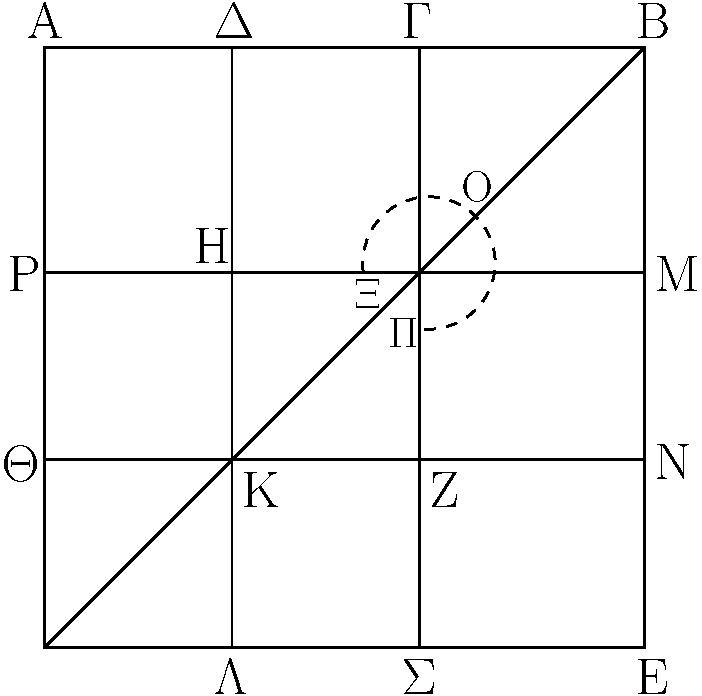
\includegraphics{Book13/fig03g.pdf}}

\gr{Εὐθεῖα γάρ τιξ ἡ ΑΒ >άκρον καὶ μέσον λόγον τετμ\kern -.7pt  ήσθω
κατὰ τὸ Γ σημεῖον, καὶ >έστω μεῖζον τμ\kern -.7pt  ῆμα
τὸ ΑΓ, καὶ τετμ\kern -.5pt  ήσθω ἡ ΑΓ δίθα κατὰ τὸ Δ; λέγω,
<ότι πενταπλάσιόν ἐστι τὸ ἀπὸ τῆξ ΒΔ τοῦ ἀπὸ
τῆξ ΔΓ.}

\gr{Ἀναγεγράφθω γὰρ ἀπὸ τῆξ ΑΒ τετράγωνον τὸ ΑΕ, καὶ
καταγεγράφθω διπλοῦν τὸ σθῆμα. ἐπεὶ διπλῆ
ἐστιν ἡ ΑΓ τῆξ ΔΓ, τετραπλάσιον >άρα τὸ ἀπὸ τῆξ ΑΓ
τοῦ ἀπὸ τῆξ ΔΓ, τουτέστι τὸ ΡΣ τοῦ ΖΗ. καὶ ἐπεὶ
τὸ ὑπὸ τῶν ΑΒΓ >ίσον ἐστὶ τῶ| ἀπὸ τῆξ ΑΓ,
καί ἐστι τὸ ὑπὸ τῶν ΑΒΓ τὸ ΓΕ, τὸ >άρα ΓΕ >ίσον
ἐστὶ τῶ| ΡΣ. τετραπλάσιον δὲ τὸ ΡΣ τοῦ ΖΗ; τετραπλάσιον
>άρα καὶ τὸ ΓΕ τοῦ ΖΗ. πάλιν ἐπεὶ >ίση ἐστὶν ἡ ΑΔ
τῆ| ΔΓ, >ίση ἐστὶ καὶ ἡ ΘΚ τῆ| ΚΖ. <ώστε καὶ τὸ ΗΖ
τετράγωνον >ίσον ἐστὶ  τῶ| ΘΛ τετραγώνῳ.
>ίση >άρα ἡ ΗΚ τῆ| ΚΛ, τουτέστιν ἡ ΜΝ τῆ| ΝΕ;
<ώστε καὶ τὸ  ΜΖ τῶ| ΖΕ ἐστιν >ίσον. ἀλλὰ
τὸ ΜΖ τῶ| ΓΗ ἐστιν >ίσον; καὶ τὸ ΓΗ >άρα τῶ| ΖΕ ἐστιν
>ίσον. κοινὸν προσκείσθω τὸ ΓΝ; ὁ >άρα ΧΟΠ γνώμων
>ίσοξ ἐστὶ τῶ| ΓΕ. ἀλλὰ τὸ ΓΕ τετραπλάσιον ἐδείθθῃ τοῦ
ΗΖ; καὶ ὁ ΧΟΠ >άρα γνώμων τετραπλάσιόξ ἐστι τοῦ ΖΗ
τετραγώνου. ὁ ΧΟΠ >άρα γνώμων καὶ τὸ ΖΗ τετράγωνον
πενταπλάσιόξ ἐστι τοῦ ΖΗ. ἀλλὰ ὁ ΧΟΠ γνώμων καὶ τὸ
ΖΗ τετράγωνόν ἐστι τὸ ΔΝ. καί
ἐστι τὸ μὲν ΔΝ τὸ ἀπὸ τῆξ ΔΒ, τὸ δὲ ΗΖ τὸ ἀπὸ
τῆξ ΔΓ. τὸ >άρα ἀπὸ τῆξ ΔΒ πενταπλάσιόν ἐστι τοῦ
ἀπὸ τῆξ ΔΓ; <όπερ >έδει δεῖχαι.}}

\ParallelRText{
\begin{center}
{\large Proposition 3}
\end{center}

If a straight-line is cut in extreme and mean ratio then the square
on the lesser piece added to half of the greater piece is five
times the square on half of the greater piece.\\

% Removed epsf size command
\centerline{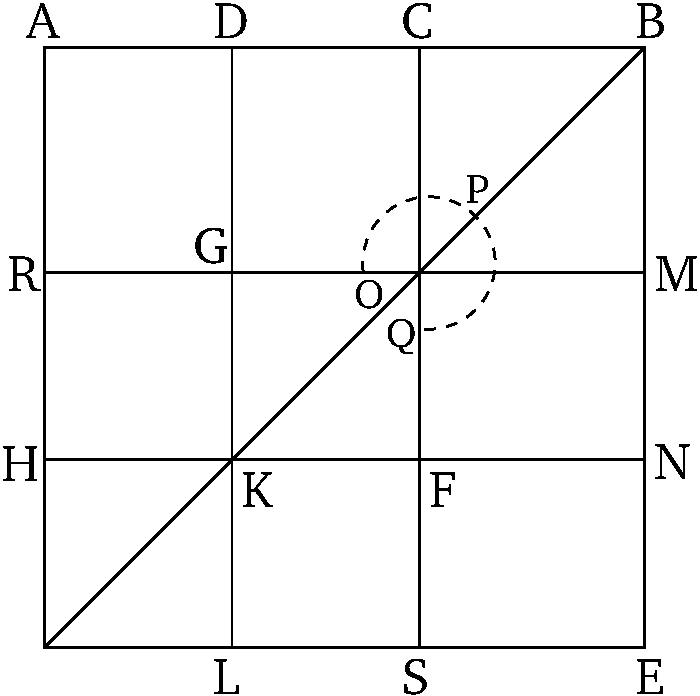
\includegraphics{Book13/fig03e.pdf}}

For let some straight-line $AB$ be cut in extreme and mean ratio
at point $C$. And let $AC$ be the greater piece. And let $AC$ be
cut in half at $D$. I say that the (square) on $BD$ is five times the
(square) on $DC$. 

For let the square $AE$ be described on $AB$. And let the
figure be drawn double. Since $AC$ is double $DC$, the
(square) on $AC$ (is) thus four times the (square) on $DC$---that
is to say, $RS$ (is four times) $FG$. And since the (rectangle contained)
by $ABC$ is equal to the (square) on $AC$ [Def.~6.3, Prop.~6.17],
and $CE$ is the (rectangle contained) by $ABC$,  $CE$ is thus equal
to $RS$. And $RS$ (is) four times $FG$. Thus, $CE$ (is) also four times
$FG$. Again, since $AD$ is equal to $DC$, $HK$ is also equal to
$KF$. Hence, square $GF$ is also equal to square $HL$. Thus,
$GK$ (is) equal to $KL$---that is to say, $MN$ to $NE$. 
Hence, $MF$ is also equal to $FE$. But, $MF$ is equal to $CG$.
Thus, $CG$ is also equal to $FE$. Let $CN$ be added to both.
Thus, gnomon $OPQ$ is equal to $CE$. But, $CE$ was shown (to be)
equal to four times $GF$. Thus, gnomon $OPQ$  is also four times
square $FG$. Thus, gnomon $OPQ$ plus square $FG$ is five times
$FG$. But, gnomon $OPQ$ plus square $FG$ is (square) $DN$. 
And  $DN$ is the (square) on $DB$, and $GF$ the (square)
on $DC$. Thus, the (square) on $DB$ is five times the (square)
on $DC$. (Which is) the very thing it was required to show.}
\end{Parallel}

%%%%
%13.4
%%%%
\pdfbookmark[1]{Proposition 13.4}{pdf13.4}
\begin{Parallel}{}{}
\ParallelLText{
\begin{center}
{\large \ggn{4}.}
\end{center}\vspace*{-7pt}

\gr{Ἐὰν εὐθεῖα γραμμ\kern -.7pt  ὴ >άκρον καὶ μέσον λόγον τμ\kern -.7pt  ηθῆ|,
τὸ ἀπὸ τῆξ <όληξ καὶ τοῦ ἐλάσσονοξ τμ\kern -.5pt  ήματοξ, τὰ συναμφότερα
τετράγωνα, τριπλάσιά ἐστι τοῦ ἀπὸ τοῦ μείζονοξ τμ\kern -.3pt  ήματοξ
τετραγώνου.}

% Removed epsf size command
\centerline{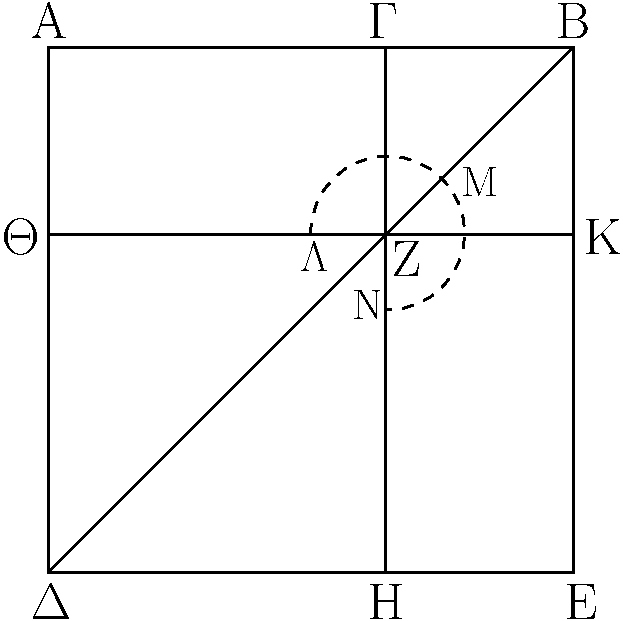
\includegraphics{Book13/fig04g.pdf}}

\gr{>'Εστω εὐθεῖα ἡ ΑΒ, καὶ τετμ\kern -.7pt  ήσθω >άκρον καὶ μέσον
λόγον κατὰ τὸ Γ, καὶ >έστω μεῖζον τμ\kern -.7pt  ῆμα τὸ ΑΓ; λέγω,
<ότι τὰ ἀπὸ τῶν ΑΒ, ΒΓ τριπλάσιά ἐστι τοῦ ἀπὸ τῆξ
ΓΑ.}

\gr{Ἀναγεγράφθω γὰρ ἀπὸ τῆξ ΑΒ τετράγωνον τὸ ΑΔΕΒ, καὶ
καταγεγράφθω τὸ σθῆμα. ἐπεὶ ο>ῦν ἡ ΑΒ >άκρον καὶ
μέσον λόγον τέτμ\kern -.7pt  ηται κατὰ τὸ Γ, καὶ τὸ μεῖζον τμ\kern -.7pt  ῆμά ἐστιν
ἡ ΑΓ, τὸ >άρα ὑπὸ τῶν ΑΒΓ >ίσον ἐστὶ τῶ| ἀπὸ τῆξ
ΑΓ. καί ἐστι τὸ μὲν ὑπὸ τῶν ΑΒΓ τὸ ΑΚ, τὸ δὲ ἀπὸ
τῆξ ΑΓ τὸ ΘΗ; >ίσον >άρα ἐστὶ τὸ ΑΚ τῶ| ΘΗ. καὶ ἐπεὶ
>ίσον ἐστὶ τὸ ΑΖ τῶ| ΖΕ, κοινὸν προσκείσθω τὸ ΓΚ; <όλον
>άρα τὸ ΑΚ <όλῳ τῶ| ΓΕ ἐστιν >ίσον; τὰ >άρα ΑΚ, ΓΕ
τοῦ ΑΚ ἐστι διπλάσια. ἀλλὰ τὰ ΑΚ, ΓΕ ὁ ΛΜΝ γνώμων
ἐστὶ καὶ τὸ ΓΚ τετράγωνον; ὁ >άρα ΛΜΝ γνώμων
καὶ τὸ ΓΚ τετράγωνον  διπλάσιά ἐστι τοῦ ΑΚ. ἀλλὰ μ\kern -.5pt  ὴν καὶ τὸ
ΑΚ τῶ| ΘΗ ἐδείθθη >ίσον; ὁ >άρα ΛΜΝ γνώμων καὶ
[τὸ ΓΚ τετράγωνον διπλάσιά ἐστι τοῦ ΘΗ; <ώστε ὁ ΛΜΝ
γνώμων καὶ] τὰ ΓΚ, ΘΗ τετράγωνα τριπλάσιά ἐστι
τοῦ ΘΗ τετραγώνου. καί ἐστιν ὁ [μὲν] ΛΜΝ γνώμων
καὶ τὰ ΓΚ, ΘΗ τετράγωνα <όλον τὸ ΑΕ καὶ τὸ ΓΚ, <άπερ
ἐστὶ τὰ ἀπὸ τῶν ΑΒ, ΒΓ τετράγωνα, τὸ δὲ ΗΘ τὸ ἀπὸ
τῆξ ΑΓ τετράγωνον. τὰ >άρα ἀπὸ τῶν ΑΒ, ΒΓ τετράγωνα
τριπλάσιά ἐστι τοῦ ἀπὸ τῆξ ΑΓ τετραγώνου; <όπερ >έδει
δεῖχαι.}}

\ParallelRText{
\begin{center}
{\large Proposition 4}
\end{center}

If a straight-line is cut in extreme and mean ratio then the sum of the
squares on the whole and the lesser piece is three times the square on
the greater piece.\\

% Removed epsf size command
\centerline{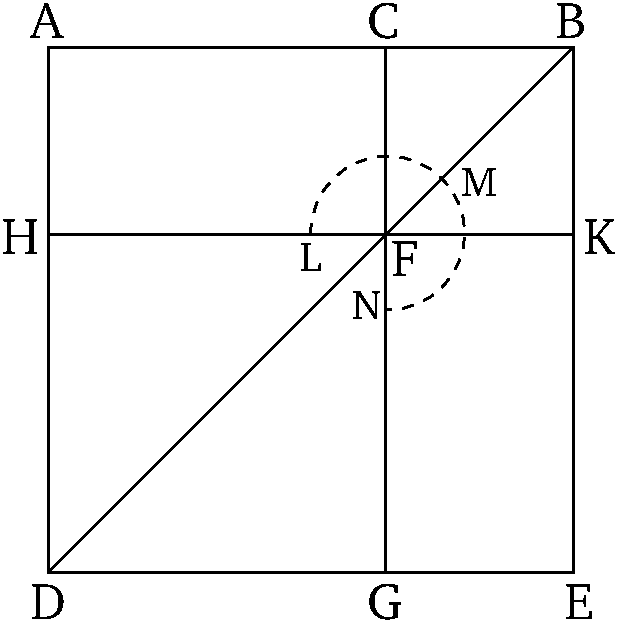
\includegraphics{Book13/fig04e.pdf}}

Let $AB$ be a straight-line, and let it be cut in extreme and mean
ratio at $C$, and let $AC$ be the greater piece. I say that the (sum of the
squares) on $AB$ and $BC$ is three times the (square) on $CA$.

For let the square $ADEB$ be described on $AB$, and
let the (remainder of the) figure be drawn. Therefore, since
$AB$ has been cut in extreme and mean ratio at $C$,  and $AC$ is the greater piece, the (rectangle contained) by $ABC$ is thus equal to the
(square) on $AC$ [Def.~6.3, Prop.~6.17]. And $AK$ is the (rectangle
contained) by $ABC$, and $HG$ the (square) on $AC$. Thus,
$AK$ is equal to $HG$.  And since $AF$ is equal to $FE$ [Prop.~1.43],
let $CK$ be added to both. Thus, the whole of $AK$  is equal to
the whole of $CE$. Thus, $AK$ plus $CE$ is double $AK$. But, $AK$
plus $CE$ is the gnomon $LMN$ plus the square $CK$. Thus, 
gnomon $LMN$ plus square $CK$ is double $AK$. But, indeed,
$AK$ was also shown (to be) equal to $HG$. Thus, gnomon $LMN$
plus [square $CK$ is double $HG$. Hence, gnomon $LMN$ plus] the
 squares $CK$ and $HG$ is three times the square $HG$.
And  gnomon $LMN$ plus the  squares  $CK$ and
$HG$ is the whole of $AE$ plus $CK$---which are the 
squares on $AB$ and $BC$ (respectively)---and $GH$ (is) the square on $AC$. 
Thus, the (sum of the) squares on $AB$ and $BC$ is three times the
square on $AC$. (Which is) the very thing it was required to show.}
\end{Parallel}

%%%%
%13.5
%%%%
\pdfbookmark[1]{Proposition 13.5}{pdf13.5}
\begin{Parallel}{}{}
\ParallelLText{
\begin{center}
{\large \ggn{5}.}
\end{center}\vspace*{-7pt}

\gr{Ἐὰν εὐθεῖα γραμμ\kern -.7pt  ὴ >άκρον καὶ μέσον λόγον τμ\kern -.7pt  ηθῆ|, καὶ
προστεθῆ| α\kern -.5pt  ὐτῆ| >ίση τῶ| μείζονι τμ\kern -.3pt  ήματι, ἡ <όλη εὐθεῖα
>άκρον καὶ μέσον λόγον τέτμ\kern -.7pt  ηται, καὶ τὸ μεῖζον τμ\kern -.7pt  ῆμά ἐστιν
ἡ ἐχ ἀρθῆξ εὐθεῖα.}

% Removed epsf size command
\centerline{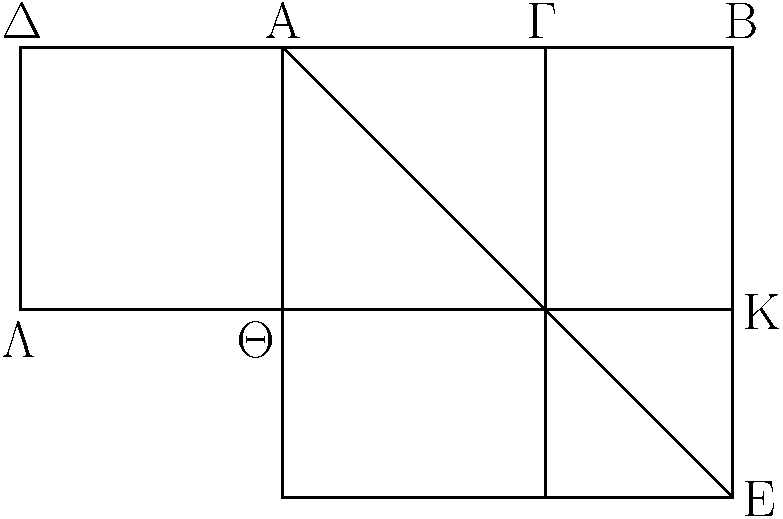
\includegraphics{Book13/fig05g.pdf}}

\gr{Εὐθεῖα γὰρ γραμμ\kern -.7pt  ὴ ἡ ΑΒ >άκρον καὶ μέσον λόγον τετμ\kern -.7pt  ήσθω
κατὰ τὸ Γ σημεῖον, καὶ >έστω μεῖζον τμ\kern -.5pt  ῆμα ἡ ΑΓ, καὶ τῆ|
ΑΓ >ίση [κείσθω] ἡ ΑΔ. λέγω, <ότι ἡ ΔΒ εὐθεῖα >άκρον
καὶ μέσον λόγον τέτμ\kern -.3pt  ηται κατὰ τὸ Α, καὶ τὸ μεῖζον τμ\kern -.7pt  ῆμά ἐστιν
ἡ ἐχ ἀρθῆξ εὐθεῖα ἡ ΑΒ.}

\gr{Ἀναγεγράφθω γὰρ ἀπὸ τῆξ ΑΒ τετράγωνον τὸ ΑΕ, καὶ
καταγεγράφθω τὸ σθῆμα. ἐπεὶ ἡ ΑΒ >άκρον καὶ μέσον
λόγον τέτμ\kern -.7pt  ηται κατὰ τὸ Γ, τὸ >άρα ὑπὸ ΑΒΓ >ίσον ἐστὶ
τῶ| ἀπὸ ΑΓ. καί ἐστι τὸ μὲν ὑπὸ ΑΒΓ τὸ ΓΕ, τὸ δὲ ἀπὸ
τῆξ ΑΓ τὸ ΓΘ; >ίσον >άρα τὸ ΓΕ τῶ| ΘΓ. ἀλλὰ τῶ| μὲν ΓΕ >ίσον
ἐστὶ τὸ ΘΕ, τῶ| δὲ ΘΓ >ίσον τὸ ΔΘ; καὶ τὸ ΔΘ >άρα >ίσον ἐστὶ
τῶ| ΘΕ [κοινὸν προσκείσθω τὸ ΘΒ]. <όλον >άρα τὸ ΔΚ <όλῳ τῶ|
ΑΕ ἐστιν >ίσον. καί ἐστι τὸ μὲν ΔΚ τὸ ὑπὸ τῶν ΒΔ, ΔΑ; >ίση
γὰρ ἡ ΑΔ τῆ| ΔΛ; τὸ δὲ ΑΕ τὸ ἀπὸ τῆξ ΑΒ; τὸ >άρα ὑπὸ
τῶν ΒΔΑ >ίσον ἐστὶ τῶ| ἀπὸ τῆξ ΑΒ. >έστιν >άρα ὡξ ἡ ΔΒ πρὸξ
τὴν ΒΑ, ο<ύτωξ ἡ ΒΑ πρὸξ τὴν ΑΔ. μείζων δὲ ἡ ΔΒ τῆξ ΒΑ;
μείζων >άρα καὶ ἡ ΒΑ τῆξ ΑΔ.}

\gr{Ἡ >άρα ΔΒ >άκρον καὶ μέσον λόγον τέτμ\kern -.7pt  ηται κατὰ τὸ Α,
καὶ τὸ μεῖζον τμ\kern -.7pt  ῆμά ἐστιν ἡ ΑΒ; <όπερ >έδει δεῖχαι.}}

\ParallelRText{
\begin{center}
{\large Proposition 5}
\end{center}

If a straight-line is cut in extreme and mean ratio, and a
(straight-line) equal to the greater piece is added to it, then the
whole straight-line has been cut in extreme and mean ratio, and
 the original straight-line is the greater piece.

% Removed epsf size command
\centerline{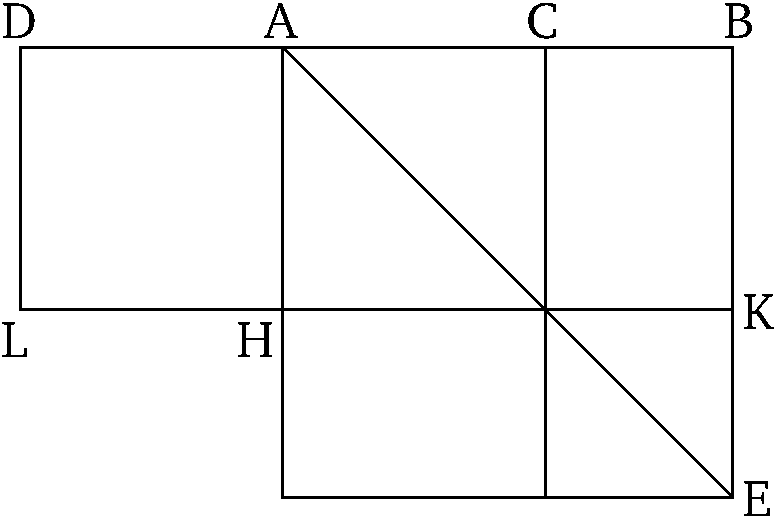
\includegraphics{Book13/fig05e.pdf}}

For let the straight-line $AB$ be cut in extreme and mean ratio
at point $C$. And let $AC$ be the greater piece. And let $AD$
be [made] equal to $AC$. I say that the straight-line $DB$ has been cut in extreme and
mean ratio at $A$, and that the original straight-line $AB$ is
the greater piece.

For let the square $AE$ be described on $AB$, and
let the (remainder of the) figure be drawn. And since
$AB$ has been cut in extreme and mean ratio at $C$, the (rectangle
contained) by $ABC$ is thus equal to the (square) on $AC$
[Def.~6.3, Prop.~6.17].  And $CE$ is the (rectangle contained)
by  $ABC$,  and $CH$ the (square) on $AC$. But, $HE$ is equal
to $CE$ [Prop.~1.43], and $DH$ equal to $HC$. Thus, $DH$ is also
equal to $HE$. [Let $HB$ be added to both.] Thus, the whole
of $DK$ is equal to the whole of $AE$. And $DK$ is the
(rectangle contained) by $BD$ and $DA$. For $AD$ (is) equal to
$DL$. And $AE$ (is) the (square) on $AB$.  Thus, the (rectangle
contained) by $BDA$ is equal to the (square) on $AB$. Thus, as
$DB$ (is) to $BA$, so $BA$ (is) to $AD$ [Prop.~6.17]. And
$DB$ (is) greater than $BA$. Thus, $BA$ (is) also greater
than $AD$ [Prop.~5.14].

Thus, $DB$ has been cut in extreme and mean ratio at $A$, and the
greater piece is $AB$. (Which is) the very thing it was required to show.}
\end{Parallel}

%%%%
%13.6
%%%%
\pdfbookmark[1]{Proposition 13.6}{pdf13.6}
\begin{Parallel}{}{}
\ParallelLText{
\begin{center}
{\large \ggn{6}.}
\end{center}\vspace*{-7pt}

\gr{Ἐὰν εὐθεῖα <ρητη >άκρον καὶ μέσον λόγον τμ\kern -.7pt  ηθῆ|, ἑκάτερον
τῶν τμ\kern -.7pt  ημάτων >άλογόξ ἐστιν ἡ καλουμένη ἀποτομ\kern -.5pt  ή.}\\

% Removed epsf size command
\centerline{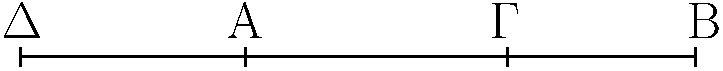
\includegraphics{Book13/fig06g.pdf}}

\gr{>'Εστω εὐθεῖα <ρητὴ ἡ ΑΒ καὶ τετμ\kern -.7pt  ήσθω >άκρον καὶ μέσον
λόγον κατὰ τὸ Γ, καὶ >έστω μεῖζον τμ\kern -.7pt  ῆμα ἡ ΑΓ; λέγω, <ότι
ἑκατέρα τῶν ΑΓ, ΓΒ >άλογόξ ἐστιν ἡ καλουμένη ἀποτομ\kern -.5pt  ή.}

\gr{Ἐκβεβλήσθω γὰρ ἡ ΒΑ, καὶ κείσθω τῆξ ΒΑ ἡμίσεια ἡ ΑΔ. ἐπεὶ
ο>ῦν εὐθεῖα ἡ ΑΒ τέτμ\kern -.7pt  ηται >άκρον
καὶ μέσον λόγον κατὰ τὸ Γ, καὶ τῶ| μείζονι τμ\kern -.7pt  ήματι τῶ| ΑΓ
πρόσκειται ἡ ΑΔ ἡμίσεια ο>ῦσα τῆξ ΑΒ, τὸ >άρα ἀπὸ ΓΔ
τοῦ ἀπὸ ΔΑ πενταπλάσιόν ἐστιν. τὸ >άρα ἀπὸ ΓΔ πρὸξ τὸ
ἀπὸ ΔΑ λόγον >έθει, <ὸν ἀριθμὸξ πρὸξ ἀριθμόν; σύμμετρον
>άρα τὸ ἀπὸ ΓΔ τῶ| ἀπὸ
ΔΑ. <ρητὸν δὲ τὸ ἀπὸ ΔΑ; <ρητὴ γάρ [ἐστιν]
ἡ ΔΑ ἡμίσεια ο>ῦσα τῆξ ΑΒ <ρητῆξ ο>ύσηξ; <ρητὸν
>άρα καὶ τὸ ἀπὸ ΓΔ; <ρητὴ >άρα ἐστὶ καὶ ἡ ΓΔ. καὶ ἐπεὶ
τὸ ἀπὸ ΓΔ πρὸξ τὸ ἀπὸ ΔΑ λόγον οὐκ >έθει, <ὸν τετράγωνοξ
ἀριθμὸξ πρὸξ τετράγωνον ἀριθμόν, ἀσύμμετροξ >άρα μ\kern -.5pt  ήκει
ἡ ΓΔ τῆ| ΔΑ; αἱ ΓΔ, ΔΑ >άρα <ρηταί εἰσι δυνάμει μόνον
σύμμετροι; ἀποτομ\kern -.3pt  ὴ >άρα ἐστὶν ἡ ΑΓ.  πάλιν, ἐπεὶ ἡ ΑΒ
>άκρον καὶ μέσον λόγον τέτμ\kern -.7pt  ηται, καὶ τὸ μεῖζον  τμ\kern -.7pt  ῆμά
ἐστιν ἡ ΑΓ, τὸ >άρα ὑπὸ ΑΒ, ΒΓ τῶ| ἀπὸ ΑΓ >ίσον
ἐστίν. τὸ >άρα ἀπὸ τῆξ ΑΓ ἀποτομ\kern -.7pt  ῆξ παρὰ τὴν ΑΒ <ρητὴν
παραβληθὲν πλάτοξ ποιεῖ τὴν ΒΓ. τὸ δὲ ἀπὸ ἀποτομ\kern -.7pt  ῆξ
παρὰ <ρητὴν παραβαλλόμενον πλάτοξ ποιεῖ ἀποτομ\kern -.7pt  ὴν πρώτην; ἀποτομ\kern -.7pt  ὴ
>άρα πρώτη ἐστὶν ἡ ΓΒ. ἐδείθθη δὲ καὶ ἡ ΓΑ ἀποτομ\kern -.7pt  ή.}

\gr{Ἐὰν >άρα εὐθεῖα <ρητὴ >άκρον καὶ μέσον λόγον τμ\kern -.7pt  ηθῆ|,
ἑκάτερον τῶν τμ\kern -.7pt  ημάτων >άλογόξ ἐστιν ἡ καλουμένη
ἀποτομ\kern -.5pt  ή; <όπερ >έδει δεῖχαι.}}

\ParallelRText{
\begin{center}
{\large Proposition 6}
\end{center}

If a rational straight-line is cut in extreme and mean ratio then each of
the pieces is that irrational (straight-line) called an apotome.

% Removed epsf size command
\centerline{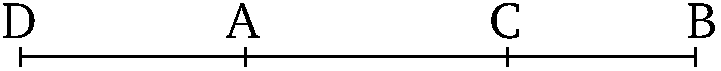
\includegraphics{Book13/fig06e.pdf}}

Let  $AB$ be a rational straight-line cut in extreme and mean ratio
at $C$, and let $AC$ be the greater piece. I say that  $AC$ and
$CB$ is each that irrational (straight-line) called an apotome.

For let $BA$ be produced, and let $AD$ be made (equal) to
half of $BA$. Therefore, since the straight-line $AB$ has been cut in
extreme and mean ratio at $C$, and $AD$, which is half of $AB$, has been added to the greater piece $AC$, the (square) on $CD$ is thus 
five times the (square) on $DA$ [Prop.~13.1]. Thus, the (square) on $CD$
has to the (square) on $DA$ the ratio which a number (has) to a number.
The (square) on $CD$ (is) thus commensurable with the (square) on
$DA$ [Prop.~10.6]. And the (square) on $DA$ (is) rational.
For $DA$ [is] rational, being half of $AB$, which is rational.
Thus, the (square) on $CD$ (is) also rational [Def.~10.4]. 
Thus, $CD$ is also rational. And since the (square) on $CD$ does not have to
the (square) on $DA$ the ratio which a square number (has) to a square
number, $CD$ (is) thus incommensurable in length with $DA$ [Prop.~10.9].
Thus, $CD$  and $DA$ are rational (straight-lines which are) commensurable in square only. Thus, $AC$ is an apotome [Prop.~10.73].  Again, since
$AB$ has been cut in extreme and mean ratio, and $AC$ is the greater
piece, the (rectangle contained) by $AB$ and $BC$ is thus equal
to the (square) on $AC$ [Def.~6.3, Prop.~6.17]. Thus, the (square) on
the apotome $AC$, applied to the rational (straight-line) $AB$, makes $BC$
as width. And the (square) on an apotome, applied to a rational
(straight-line), makes a first apotome as width [Prop.~10.97].
Thus, $CB$ is a first apotome. And $CA$ was also
shown (to be) an apotome.

Thus, if a rational straight-line is cut in extreme and mean ratio then each of
the pieces is that irrational (straight-line) called an apotome.}
\end{Parallel}

%%%%
%13.7
%%%%
\pdfbookmark[1]{Proposition 13.7}{pdf13.7}
\begin{Parallel}{}{}
\ParallelLText{
\begin{center}
{\large \ggn{7}.}
\end{center}\vspace*{-7pt}

\gr{Ἐὰν πενταγώνου ἰσοπλεύρου αἱ τρεῖξ γωνίαι >ήτοι αἱ κατὰ
τὸ ἑχῆξ >ὴ αἱ μ\kern -.7pt  ὴ κατὰ τὸ ἑχῆξ >ίσαι >ῶσιν, ἰσογώνιον >έσται
τὸ πεντάγωνον.}

\gr{Πενταγώνου γὰρ ἰσοπλεύρον τοῦ ΑΒΓΔΕ αἱ τρεῖξ γωνίαι
πρότερον αἱ κατὰ τὸ ἑχῆξ αἱ πρὸξ τοῖξ Α, Β, Γ >ίσαι ἀλλήλαιξ
>έστωσαν; λέγω, <ότι ἰσογώνιόν ἐστι τὸ ΑΒΓΔΕ πεντάγωνον.}

\gr{Ἐπεζεύθθωσαν γὰρ αἱ ΑΓ, ΒΕ, ΖΔ. καὶ ἐπεὶ δύο αἱ ΓΒ, ΒΑ
δυσὶ ταῖξ ΒΑ, ΑΕ >ίσαι ἐισὶν ἑκατέρα ἑκατέρᾳ, καὶ γωνία ἡ ὑπὸ ΓΒΑ γωνίᾳ
τῆ| ὑπὸ ΒΑΕ ἐστιν >ίση, βάσιξ >άρα ἡ ΑΓ βάσει τῆ| ΒΕ ἐστιν
>ίση, καὶ τὸ ΑΒΓ τρίγωνον τῶ| ΑΒΕ τριγώνῳ >ίσον, καὶ αἱ
λοιπαὶ γωνίαι ταῖξ λοιπαῖξ γωνίαιξ >ίσαι >έσονται, ὑφ> <ὰξ αἱ
>ίσαι πλευραὶ ὑποτείνουσιν, ἡ μὲν ὑπὸ ΒΓΑ τῆ| ὑπὸ ΒΕΑ,
ἡ δὲ ὑπὸ ΑΒΕ τῆ| ὑπὸ ΓΑΒ; <ώστε καὶ πλευρὰ ἡ ΑΖ πλευρᾶ|
τῆ| ΒΖ ἐστιν >ίση. ἐδείθθη δὲ καὶ <όλη ἡ ΑΓ <όλῃ τῆ|
ΒΕ >ίση; καὶ λοιπὴ >άρα ἡ ΖΓ λοιπῆ| τῆ| ΖΕ ἐστιν >ίση. >έστι
δὲ καὶ ἡ ΓΔ τῆ| ΔΕ >ίση. δύο δὴ αἱ ΖΓ, ΓΔ δυσὶ ταῖξ
ΖΕ, ΕΔ >ίσαι εἰσίν; καὶ βάσιξ α\kern -.7pt  ὐτῶν κοινὴ ἡ ΖΔ; γωνία
>άρα ἡ ὑπὸ ΖΓΔ γωνίᾳ τῆ| ὑπὸ ΖΕΔ ἐστιν >ίση. ἐδείθθη
δὲ καὶ ἡ ὑπὸ ΒΓΑ τῆ| ὑπὸ ΑΕΒ >ίση; καὶ <όλη >άρα ἡ ὑπὸ
ΒΓΔ <όλῃ τῆ| ὑπὸ ΑΕΔ >ίση. ἀλλ> ἡ ὑπὸ ΒΓΔ >ίση ὑπόκειται
ταῖξ πρὸξ τοῖξ Α, Β γωνίαιξ; καὶ ἡ ὑπὸ ΑΕΔ >άρα ταῖξ πρὸξ
τοῖξ Α, Β γωνίαιξ >ίση ἐστίν. ὁμοίωξ δὴ δείχομεν, <ότι
καὶ ἡ ὑπὸ ΓΔΕ γωνία >ίση ἐστὶ ταῖξ πρὸξ τοῖξ Α, Β, Γ γωνίαιξ;
ἰσογώνιον >άρα ἐστὶ τὸ ΑΒΓΔΕ πεντάγωνον.}\\~\\

% Removed epsf size command
\centerline{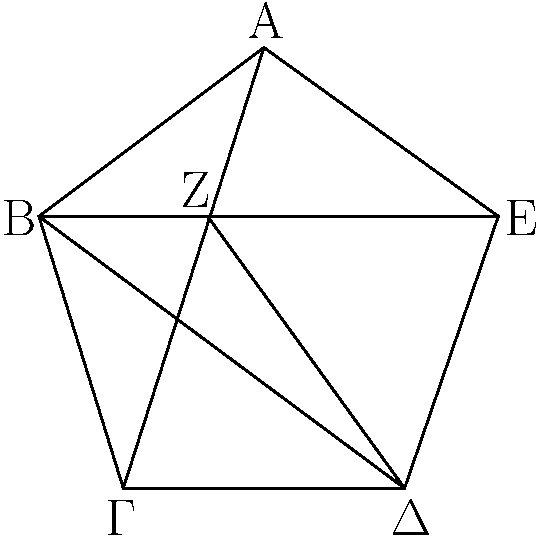
\includegraphics{Book13/fig07g.pdf}}

\gr{Ἀλλὰ δὴ μ\kern -.7pt  ὴ >έστωσαν >ίσαι αἱ κατὰ τὸ ἑχῆξ γωνίαι,
ἀλλ> >έστωσαν >ίσαι αἱ πρὸξ τοῖξ Α, Γ, Δ σημείοιξ;
λέγω, <ότι καὶ ο<ύτωξ ἰσογώνιόν ἐστι τὸ ΑΒΓΔΕ πεντάγωνον.}

\gr{Ἐπεζεύθθω γὰρ ἡ ΒΔ. καὶ ἐπεὶ δύο αἱ ΒΑ, ΑΕ δυσὶ ταῖξ
ΒΓ, ΓΔ >ίσαι εἰσὶ καὶ γωνίαξ >ίσαξ περιέθουσιν, βάσιξ >άρα ἡ ΒΕ βάσει τῆ| ΒΔ >ίση ἐστίν, καὶ τὸ ΑΒΕ τρίγωνον τῶ| ΒΓΔ τριγώνῳ
>ίσον ἐστίν, καὶ αἱ λοιπαὶ γωνίαι ταῖξ λοιπαῖξ γωνίαιξ
>ίσαι >έσονται, ὑφ>  <ὰξ αἱ >ίσαι πλευραὶ ὑποτείνουσιν; >ίση
>άρα ἐστὶν ἡ ὑπὸ ΑΕΒ γωνία τῆ| ὑπὸ ΓΔΒ. >έστι δὲ καὶ ἡ
ὑπὸ ΒΕΔ γωνία τῆ| ὑπὸ ΒΔΕ >ίση, ἐπεὶ καὶ πλευρὰ
ἡ ΒΕ πλευρᾶ| τῆ| ΒΔ ἐστιν >ίση.
 καὶ <όλη >άρα ἡ ὑπὸ
ΑΕΔ γωνία <όλῃ τῆ| ὑπὸ ΓΔΕ ἐστιν  >ίση. ἀλλὰ ἡ ὑπὸ
ΓΔΕ ταῖξ πρὸξ τοῖξ Α, Γ γωνίαιξ ὑπόκειται >ίση;  καὶ ἡ ὑπὸ
ΑΕΔ >άρα γωνία ταῖξ πρὸξ τοῖξ Α, Γ >ίση ἐστίν. διὰ τὰ α\kern -.7pt  ὐτὰ
δὴ καὶ ἡ ὑπὸ ΑΒΓ >ίση ἐστὶ ταῖξ πρὸξ τοῖξ Α, Γ, Δ γωνίαιξ.
ἰσογώνιον >άρα ἐστὶ τὸ ΑΒΓΔΕ πεντάγωνον; <όπερ >έδει
δεῖχαι.}}

\ParallelRText{
\begin{center}
{\large Proposition 7}
\end{center}

If  three angles, either  consecutive or not consecutive, of an equilateral pentagon
are equal then the pentagon will be equiangular.

For let three angles of the equilateral pentagon $ABCDE$---first of
all, the consecutive (angles) at $A$, $B$, and $C$----be equal to
one another. I say that pentagon $ABCDE$ is equiangular.

For let $AC$, $BE$, and $FD$ be joined. And since the two (straight-lines) $CB$ and $BA$ are equal to the two (straight-lines) $BA$ and
$AE$, respectively, and angle $CBA$ is equal to angle $BAE$,  base
$AC$ is thus equal to base $BE$, and triangle $ABC$  equal to triangle
$ABE$, and the remaining angles will be equal to the remaining angles
which the equal sides subtend [Prop.~1.4],  (that is), $BCA$ (equal) to $BEA$, and $ABE$ to $CAB$. And hence side $AF$ is also equal to side $BF$ [Prop.~1.6]. And the whole  of $AC$ was also shown (to be) equal to
the whole of $BE$. Thus, the remainder $FC$ is also equal to the remainder $FE$.
And $CD$ is also equal to $DE$. So, the two (straight-lines) $FC$ and
$CD$ are equal to the two (straight-lines) $FE$ and $ED$ (respectively). 
And $FD$ is their common base. Thus, angle $FCD$ is equal to angle
$FED$ [Prop.~1.8]. And $BCA$ was also shown (to be) equal to 
$AEB$. And thus the whole of  $BCD$ (is) equal to the whole of $AED$.
But, (angle) $BCD$ was assumed (to be) equal to the angles at $A$ and
$B$. Thus, (angle) $AED$ is also equal to the angles at $A$ and $B$. So, 
similarly, we can show that angle $CDE$ is also equal to the angles
at $A$, $B$, $C$. Thus, pentagon $ABCDE$ is equiangular.

% Removed epsf size command
\centerline{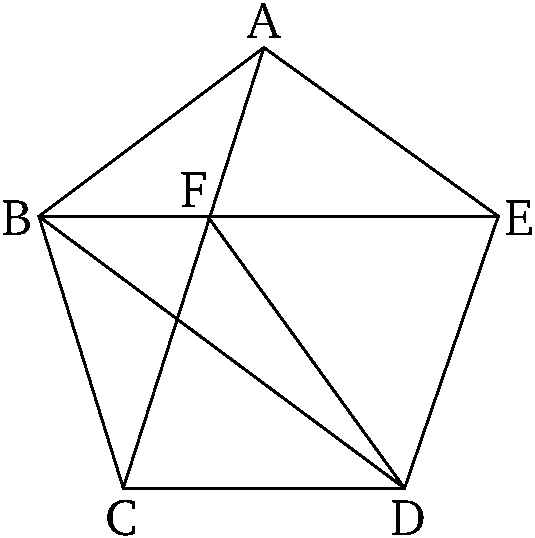
\includegraphics{Book13/fig07e.pdf}}

And so let consecutive  angles not be equal, but let
the (angles) at points $A$, $C$, and $D$ be equal. I say that pentagon $ABCDE$ is also
equiangular in this case.

For let $BD$ be joined. And since the two (straight-lines) $BA$
and $AE$ are equal to the (straight-lines) $BC$ and $CD$, and they contain
equal angles,   base $BE$ is thus equal to base $BD$, and triangle $ABE$
is equal to triangle $BCD$, and the remaining angles will be equal
to the remaining angles which the equal sides subtend [Prop.~1.4]. 
Thus, angle $AEB$ is equal to (angle) $CDB$. And angle $BED$
is also equal to (angle) $BDE$,  since side $BE$ is also equal to side
$BD$ [Prop.~1.5]. Thus, the whole angle $AED$ is also equal to the
whole (angle) $CDE$. But, (angle) $CDE$ was assumed (to be) equal
to the angles at $A$ and $C$.  Thus, angle $AED$ is also equal to the (angles)
at $A$ and $C$. So, for the same (reasons), (angle) $ABC$ is also equal
to the angles at  $A$, $C$, and $D$. Thus, pentagon $ABCDE$ is equiangular.
(Which is) the very thing it was required to show.}
\end{Parallel}

%%%%
%13.8
%%%%
\pdfbookmark[1]{Proposition 13.8}{pdf13.8}
\begin{Parallel}{}{}
\ParallelLText{
\begin{center}
{\large \ggn{8}.}
\end{center}\vspace*{-7pt}

\gr{Ἐὰν πενταγώνου ἰσοπλεύρου καὶ ἰσογωνίου τὰξ κατὰ
τὸ ἑχῆξ δύο γωνίαξ ὑποτείνωσιν εὐθεῖαι, >άκρον καὶ
μέσον λόγον τέμνουσιν ἀλλήλαξ, καὶ τὰ μείζονα α\kern -.7pt  ὐτῶν
τμ\kern -.7pt  ήματα >ίσα ἐστὶ τῆ| τοῦ πενταγώνου πλευρᾶ|.}

\gr{Πενταγώνου γὰρ ἰσοπλεύρον καὶ ἰσογωνίου τοῦ ΑΒΓΔΕ δύο
γωνίαξ τὰξ κατὰ τὸ ἑχῆξ τὰξ πρὸξ τοῖξ Α, Β ὑποτεινέτωσαν εὐθεῖαι
αἱ ΑΓ, ΒΕ τέμνουσαι ἀλλήλαξ κατὰ τὸ Θ σημεὶον; λέγω, <ότι
ἑκατέρα α\kern -.7pt  ὐτῶν >άκρον καὶ μέσον λόγον τέτμ\kern -.7pt  ηται κατὰ τὸ Θ
σημεῖον, καὶ τὰ μείζονα α\kern -.5pt  ὐτῶν τμ\kern -.3pt  ήματα >ίσα ἐστὶ τῆ| τοῦ
πενταγώνου πλευρᾶ|.}

% Removed epsf size command
\centerline{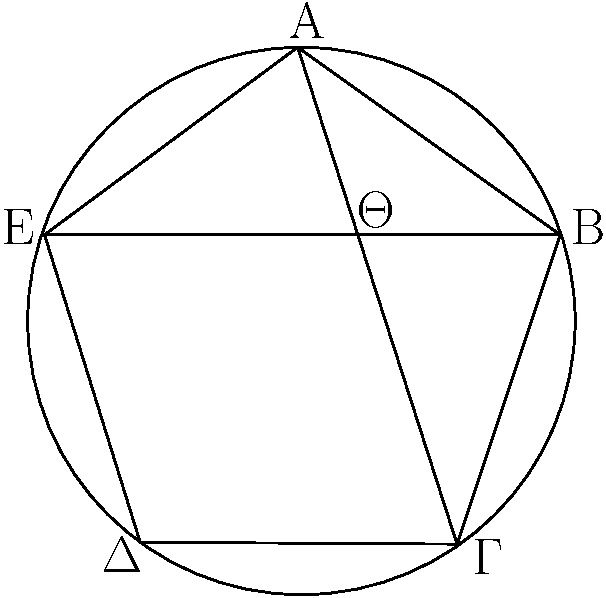
\includegraphics{Book13/fig08g.pdf}}

\gr{Περιγεγράφθω γὰρ περὶ τὸ ΑΒΓΔΕ πεντάγωνον κύκλοξ ὁ
ΑΒΓΔΕ. καὶ ἐπεὶ δύο εὐθεῖαι αἱ ΕΑ, ΑΒ δυσὶ ταῖξ ΑΒ, ΒΓ
>ίσαι εἰσὶ καὶ γωνίαξ >ίσαξ περιέθουσιν, βάσιξ >άρα ἡ ΒΕ βάσει
τῆ| ΑΓ >ίση ἐστίν, καὶ τὸ ΑΒΕ τρίγωνον τῶ| ΑΒΓ τριγώνῳ
>ίσον ἐστίν, καὶ αἱ λοιπαὶ γωνίαι ταῖξ λοιπαῖξ γωνίαιξ
>ίσαι >έσονται ἑκατέρα ἑκατέρᾳ, ὑφ> <ὰξ αἱ >ίσαι πλευραὶ
ὑποτείνουσιν. >ίση >άρα ἐστὶν ἡ ὑπὸ ΒΑΓ γωνία τῆ|
ὑπὸ ΑΒΕ; διπλῆ >άρα ἡ ὑπὸ ΑΘΕ τῆξ ὑπὸ ΒΑΘ. >έστι
δὲ καὶ ἡ ὑπὸ ΕΑΓ τῆξ ὑπὸ ΒΑΓ διπλῆ, ἐπειδήπερ καὶ
περιφέρεια ἡ ΕΔΓ περιφερείαξ τῆξ ΓΒ ἐστι διπλῆ; >ίση >άρα
ἡ ὑπὸ ΘΑΕ γωνία τῆ| ὑπὸ ΑΘΕ; <ώστε καὶ ἡ ΘΕ εὐθεῖα
τῆ| ΕΑ, τουτέστι τῆ| ΑΒ ἐστιν >ίση. καὶ ἐπεὶ >ίση
ἐστὶν ἡ ΒΑ εὐθεῖα τῆ| ΑΕ, >ίση ἐστὶ καὶ γωνία ἡ ὑπὸ
ΑΒΕ τῆ| ὑπὸ ΑΕΒ. ἀλλὰ ἡ ὑπὸ ΑΒΕ τῆ| ὑπὸ ΒΑΘ
ἐδείθθη >ίση; καὶ ἡ ὑπὸ ΒΕΑ >άρα τῆ| ὑπὸ ΒΑΘ
ἐστιν >ίση. καὶ κοινὴ τῶν δύο τριγώνων τοῦ τε ΑΒΕ καὶ
τοῦ ΑΒΘ ἐστιν ἡ ὑπὸ ΑΒΕ; λοιπὴ >άρα ἡ ὑπὸ ΒΑΕ
γωνία λοιπῆ| τῆ| ὑπὸ ΑΘΒ ἐστιν >ίση; ἰσογώνιον >άρα
ἐστὶ τὸ ΑΒΕ τρίγωνον τῶ| ΑΒΘ τριγώνῳ; ἀνάλογον >άρα
ἐστὶν ὡξ ἡ ΕΒ πρὸξ τὴν ΒΑ, ο<ύτωξ ἡ ΑΒ πρὸξ
τὴν ΒΘ. >ίση δὲ ἡ ΒΑ τῆ| ΕΘ; ὡξ >άρα ἡ ΒΕ πρὸξ τὴν
ΕΘ, ο<ύτωξ ἡ ΕΘ πρὸξ τὴν ΘΒ. μείζων δὲ ἡ ΒΕ
τῆξ ΕΘ; μείζων >άρα καὶ ἡ ΕΘ τῆξ ΘΒ. ἡ ΒΕ
<άρα >άκρον καὶ μέσον λόγον τέτμ\kern -.7pt  ηται κατὰ τὸ Θ, καὶ τὸ
μεῖζον τμ\kern -.7pt  ῆμα τὸ ΘΕ >ίσον ἐστὶ τῆ| τοῦ πενταγώνου
πλευρᾶ|. ὁμοίωξ δὴ  δείχομεν, <ότι καὶ ἡ ΑΓ
>άκρον καὶ μέσον λόγον τέτμ\kern -.5pt  ηται κατὰ τὸ Θ, καὶ τὸ μεῖζον α\kern -.3pt  ὐτῆξ
τμ\kern -.7pt  ῆμα ἡ ΓΘ >ίσον ἐστὶ τῆ| τοῦ πενταγώνου πλευρᾶ|; <όπερ
>έδει δεῖχαι.}}

\ParallelRText{
\begin{center}
{\large Proposition 8}
\end{center}

If straight-lines subtend two consecutive angles of an equilateral and equiangular pentagon then they cut one another in extreme and
mean ratio, and their greater pieces are equal to  the sides of the pentagon.

For let the two straight-lines, $AC$ and $BE$, cutting one another
at point $H$, have subtended  two consecutive angles, at $A$ and $B$ (respectively), of
the equilateral and equiangular pentagon $ABCDE$. I say that
each of them has been cut in extreme and mean ratio at point $H$, and
that their greater pieces are equal to the sides of the pentagon.

% Removed epsf size command
\centerline{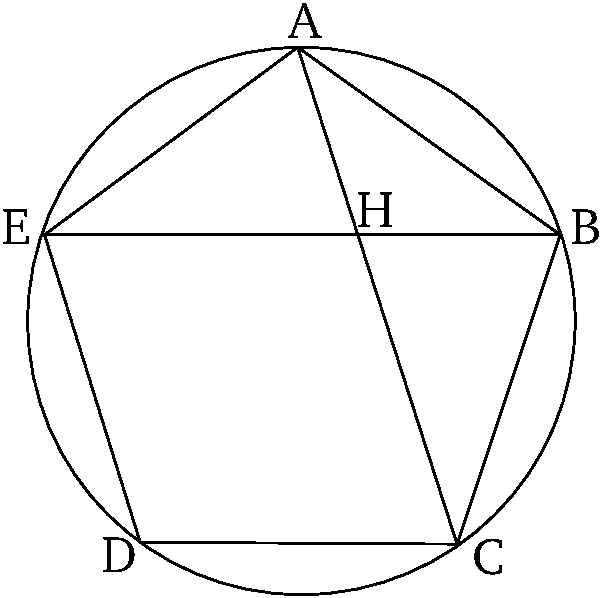
\includegraphics{Book13/fig08e.pdf}}

For let the circle $ABCDE$ be circumscribed about pentagon
$ABCDE$ [Prop.~4.14]. And since the two straight-lines $EA$ and
$AB$ are equal to the two (straight-lines) $AB$ and $BC$ (respectively),
and they contain equal angles, the base $BE$ is thus equal to the base
$AC$, and triangle $ABE$ is equal to triangle $ABC$, and the remaining
angles will be equal to the remaining angles, respectively,
which the equal sides subtend [Prop.~1.4]. Thus, angle $BAC$ is equal
to (angle) $ABE$. Thus, (angle) $AHE$ (is) double (angle) $BAH$ [Prop.~1.32]. And $EAC$ is also double $BAC$, inasmuch as
circumference $EDC$ is also double circumference $CB$ [Props.~3.28, 6.33].
Thus, angle $HAE$ (is) equal to (angle) $AHE$. Hence, straight-line
$HE$ is also equal to (straight-line) $EA$---that is to say, to (straight-line)
$AB$ [Prop.~1.6]. And since straight-line $BA$ is equal to $AE$,
angle $ABE$ is also equal to $AEB$ [Prop.~1.5]. But, $ABE$
was shown (to be) equal to $BAH$. Thus, $BEA$ is also equal to
$BAH$. And (angle) $ABE$ is common to the two triangles
$ABE$ and $ABH$. Thus, the remaining angle $BAE$ is equal to
the remaining (angle) $AHB$ [Prop.~1.32]. Thus, triangle $ABE$
is equiangular to triangle $ABH$. Thus, proportionally, as $EB$ is
to $BA$, so $AB$ (is) to $BH$ [Prop.~6.4].  And $BA$ (is) equal to
$EH$. Thus, as $BE$ (is) to $EH$, so $EH$ (is) to $HB$. And
$BE$ (is) greater than $EH$.  $EH$ (is) thus also greater than $HB$
[Prop.~5.14]. Thus, $BE$ has been cut in extreme and mean ratio at
$H$, and the greater piece $HE$ is equal to the side of the pentagon. 
So, similarly, we can show that $AC$ has also been cut in extreme and
mean ratio at $H$, and that  its greater piece $CH$ is equal to the side
of the pentagon. (Which is) the very thing it was required to show.}
\end{Parallel}

%%%%
%13.9
%%%%
\pdfbookmark[1]{Proposition 13.9}{pdf13.9}
\begin{Parallel}{}{}
\ParallelLText{
\begin{center}
{\large \ggn{9}.}
\end{center}\vspace*{-7pt}

\gr{Ἐὰν ἡ τοῦ ἑχαγώνου πλευρὰ καὶ ἡ τοῦ δεκαγώνου τῶν
εἰξ τὸν α\kern -.7pt  ὐτὸν κύκλον ἐγγραφομένων συντεθῶσιν, ἡ
<όλη εὐθεῖα >άκρον καὶ μέσον λόγον τέτμ\kern -.7pt  ηται, καὶ τὸ
μεῖχον α\kern -.5pt  ὐτῆξ τμ\kern -.3pt  ῆμά ἐστιν ἡ τοῦ ἑχαγώνου πλευρά.}\\

\gr{>'Εστω κύκλοξ ὁ ΑΒΓ, καὶ τῶν εἰξ τὸν ΑΒΓ κύκλον ἐγγραφομένων
σθημάτων, δεκαγώνου μὲν >έστω πλευρὰ ἡ ΒΓ, ἑχαγώνου δὲ
ἡ ΓΔ, καὶ >έστωσαν ἐπ>
εὐθείαξ; λέγω, <ότι ἡ <όλη εὐθεῖα ἡ ΒΔ >άκρον καὶ μέσον
λόγον τέτμ\kern -.7pt  ηται, καὶ τὸ μεῖζον α\kern -.7pt  ὐτῆξ τμ\kern -.5pt  ῆμά
ἐστιν ἡ ΓΔ.}

% Removed epsf size command
\centerline{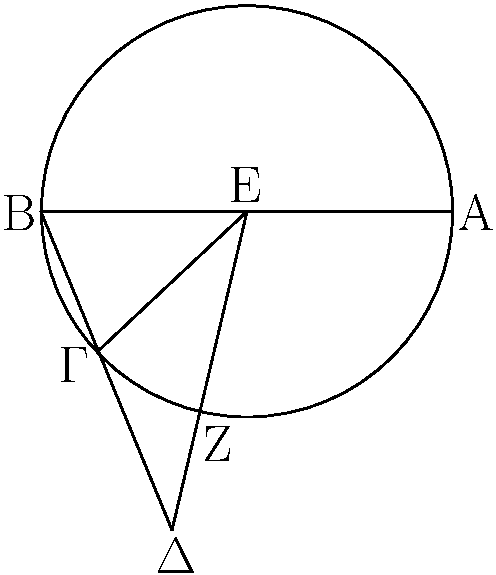
\includegraphics{Book13/fig09g.pdf}}

\gr{Εἰλήφθω γὰρ τὸ κέντρον τοῦ κύκλου τὸ Ε σημεῖον,
καὶ ἐπεζεύθθωσαν αἱ ΕΒ, ΕΓ, ΕΔ, καὶ διήθθω ἡ ΒΕ ἐπὶ
τὸ Α. ἐπεὶ δεκαγώνου ἰσοπλεύρον πλευρά ἐστιν ἡ ΒΓ,
πενταπλασίων >άρα ἡ ΑΓΒ περιφέρεια
τῆξ ΒΓ περιφερείαξ; τετραπλασίων >άρα ἡ ΑΓ περιφέρεια τῆξ
ΓΒ. ὡξ δὲ ἡ ΑΓ περιφέρεια πρὸξ τὴν
ΓΒ, ο<ύτωξ ἡ ὑπὸ ΑΕΓ γωνία πρὸξ τὴν ὑπὸ ΓΕΒ;
τετραπλασίων >άρα ἡ ὑπὸ ΑΕΓ τῆξ ὑπὸ ΓΕΒ. καὶ
ἐπεὶ >ίση ἡ ὑπὸ ΕΒΓ γωνία τῆ| ὑπὸ ΕΓΒ, ἡ
>άρα ὑπὸ ΑΕΓ γωνία διπλασία ἐστὶ τῆξ ὑπὸ ΕΓΒ. καὶ
ἐπεὶ >ίση ἐστὶν ἡ ΕΓ εὐθεῖα τῆ| ΓΔ; ἑκατέρα γὰρ
α\kern -.7pt  ὐτῶν >ίση ἐστὶ τῆ| τοῦ ἑχαγώνου πλευρᾶ| τοῦ εἰξ
τὸν ΑΒΓ κύκλον [ἐγγραφομένου]; >ίση ἐστὶ καὶ ἡ
ὑπὸ ΓΕΔ γωνία τῆ| ὑπὸ ΓΔΕ γωνίᾳ; διπλασία >άρα ἡ
ὑπὸ ΕΓΒ γωνία τῆξ ὑπὸ ΕΔΓ. ἀλλὰ τῆξ ὑπὸ ΕΓΒ
διπλασία ἐδείθθη ἡ ὑπὸ ΑΕΓ; τετραπλασία >άρα ἡ ὑπὸ
ΑΕΓ τῆξ ὑπὸ ΕΔΓ. ἐδείθθη δὲ καὶ τῆξ ὑπὸ ΒΕΓ τετραπλασία
ἡ ὑπὸ ΑΕΓ; >ίση >άρα ἡ ὑπὸ ΕΔΓ τῆ| ὑπὸ ΒΕΓ. κοινὴ
δὲ τῶν δύο τριγώνων, τοῦ τε
ΒΕΓ καὶ τοῦ ΒΕΔ, ἡ ὑπὸ ΕΒΔ γωνία;
καὶ λοιπὴ >άρα ἡ ὑπὸ ΒΕΔ τῆ| ὑπὸ ΕΓΒ ἐστιν >ίση;
ἰσογώνιον >άρα ἐστὶ τὸ ΕΒΔ τρίγωνον τῶ| ΕΒΓ τριγώνῳ.
ἀνάλογον >άρα ἐστὶν ὡξ ἡ ΔΒ πρὸξ τὴν ΒΕ, ο<ύτωξ
ἡ ΕΒ πρὸξ τὴν ΒΓ. >ίση δὲ ἡ ΕΒ τῆ| ΓΔ. >έστιν
>άρα ὡξ ἡ ΒΔ πρὸξ τὴν ΔΓ, ο<ύτωξ ἡ ΔΓ πρὸξ τὴν ΓΒ.
μείζων δὲ ἡ ΒΔ τῆξ ΔΓ; μείζων >άρα καὶ ἡ ΔΓ
τῆξ ΓΒ. ἡ ΒΔ >άρα εὐθεῖα >άκρον καὶ μέσον λόγον
τέτμ\kern -.7pt  ηται [κατὰ τὸ Γ], καὶ τὸ μεῖζον τμ\kern -.5pt  ῆμα α\kern -.3pt  ὐτῆξ
ἐστιν ἡ ΔΓ; <όπερ >έδει δεῖχαι.}}

\ParallelRText{
\begin{center}
{\large Proposition 9}
\end{center}

If the side of a hexagon and  of a decagon inscribed in the same circle
are added together then the whole straight-line has been cut in extreme and
mean ratio (at the junction point), and its greater piece is the side of the hexagon.$^\dag$

Let $ABC$ be a circle. And of the figures inscribed in circle $ABC$, 
let $BC$ be the side of a decagon, and $CD$ (the side) of a hexagon.
And let them be (laid down) straight-on (to one another). I say that
the whole straight-line $BD$ has been cut in extreme and mean
ratio (at $C$), and that   $CD$ is its greater piece. \\

% Removed epsf size command
\centerline{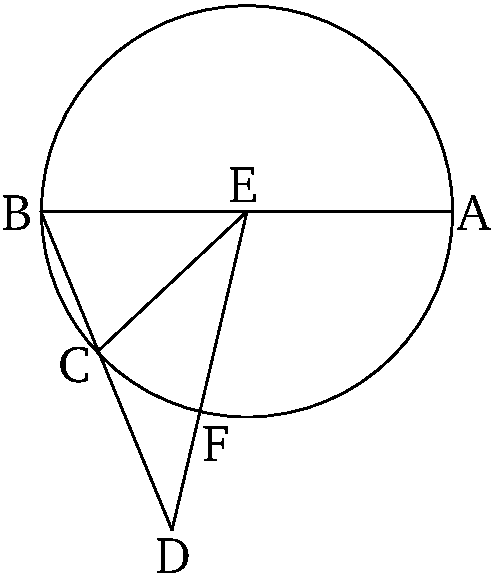
\includegraphics{Book13/fig09e.pdf}}

For let the center of the circle, point $E$, be found [Prop.~3.1],
and let $EB$, $EC$, and $ED$ be joined, and let $BE$ be
drawn across to $A$. Since $BC$ is a side on an equilateral decagon,
circumference $ACB$ (is) thus five times circumference $BC$. Thus,
circumference $AC$ (is) four times $CB$. And as circumference $AC$
(is) to $CB$, so angle $AEC$ (is) to $CEB$ [Prop.~6.33]. Thus,
(angle) $AEC$ (is) four times $CEB$. And since angle $EBC$
(is) equal to $ECB$ [Prop.~1.5], angle $AEC$ is thus double $ECB$ [Prop.~1.32]. 
And since straight-line $EC$ is equal to $CD$---for each of them is equal
to the side of the hexagon [inscribed] in circle $ABC$ [Prop.~4.15~corr.]---
angle $CED$ is also equal to angle $CDE$ [Prop.~1.5]. Thus,
angle $ECB$ (is) double $EDC$ [Prop.~1.32]. But,
$AEC$ was shown (to be) double $ECB$. Thus, $AEC$ (is) four times
$EDC$. And $AEC$ was also shown (to be) four times $BEC$. 
Thus, $EDC$ (is) equal to $BEC$. And angle $EBD$ (is) common
to the two triangles $BEC$ and $BED$. Thus, the remaining (angle)
$BED$ is equal to the (remaining angle) $ECB$ [Prop.~1.32]. 
Thus, triangle $EBD$ is equiangular to triangle $EBC$. Thus,
proportionally, as $DB$ is to $BE$, so $EB$ (is) to $BC$ [Prop.~6.4].
And $EB$ (is) equal to $CD$. Thus, as $BD$ is to $DC$, so $DC$
(is) to $CB$. And $BD$ (is) greater than $DC$. Thus,
$DC$ (is) also greater than $CB$ [Prop.~5.14]. Thus, the
straight-line $BD$ has been cut in extreme and mean ratio [at $C$],
and $DC$  is its greater piece. (Which is), the very thing it was required to show.}
\end{Parallel}{\footnotesize\noindent$^\dag$ If the circle is of unit radius
then the side of the hexagon is 1, whereas the side of the decagon is $(1/2)\,(\sqrt{5}-1)$.}

%%%%
%13.10
%%%%
\pdfbookmark[1]{Proposition 13.10}{pdf13.10}
\begin{Parallel}{}{}
\ParallelLText{
\begin{center}
{\large \ggn{10}.}
\end{center}\vspace*{-7pt}

\gr{Ἐὰν εἰξ κύκλον πεντάγωνον ἰσόπλευρον ἐγγραφῆ|, ἡ τοῦ
πενταγώνου πλευρὰ δύναται τήν τε τοῦ ἑχαγώνου καὶ τὴν τοῦ
δεκαγώνου τῶν εἰξ τὸν α\kern -.7pt  ὐτὸν κύκλον ἐγγραφομένων.}\\

% Removed epsf size command
\centerline{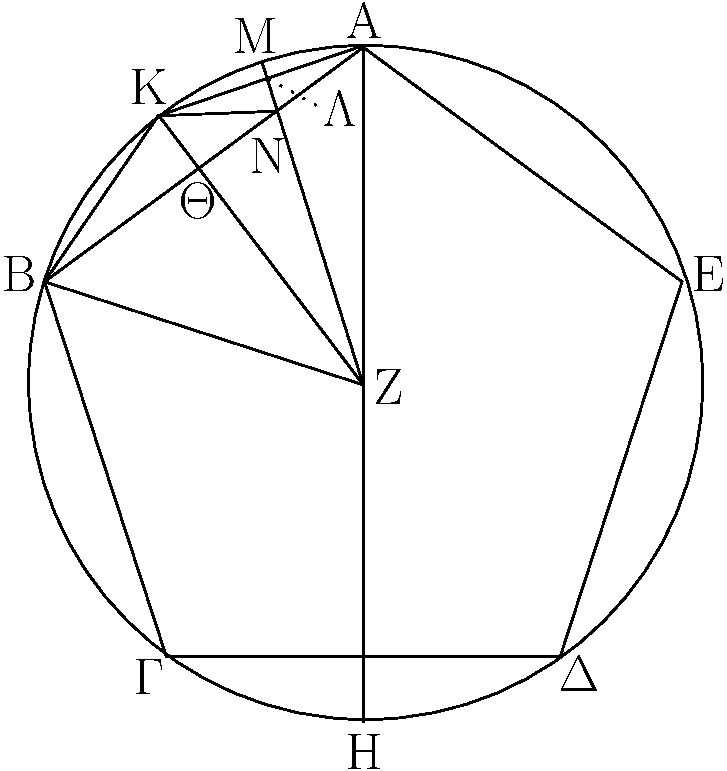
\includegraphics{Book13/fig10g.pdf}}

\gr{>'Εστω κύκλοξ ὁ ΑΒΓΔΕ, καὶ εἰξ τὸ ΑΒΓΔΕ κύκλον
πεντάγωνον ἰσόπλευρον ἐγγεγράφθω τὸ ΑΒΓΔΕ. λέγω,
<ότι ἡ τοῦ ΑΒΓΔΕ πενταγώνου πλευρὰ δύναται τήν τε τοῦ
ἑχαγώνου καὶ τὴν τοῦ δεκαγώνου πλευρὰν τῶν εἰξ
τὸν ΑΒΓΔΕ κύκλον ἐγγραφομένων.}

\gr{Εἰλήφθω γὰρ τὸ κέντρον τοῦ κύκλου τὸ Ζ σημεὶον, καὶ
ἐπιζευθθεῖσα ἡ ΑΖ διήθθω ἐπὶ τὸ Η σημεῖον, καὶ ἐπεζεύθθω
ἡ ΖΒ, καὶ ἀπὸ τοῦ Ζ ἐπὶ τὴν ΑΒ κάθετοξ >ήθθω ἡ ΖΘ,
καὶ διήθθω ἐπὶ τὸ Κ, καὶ ἐπεζεύθθωσαν αἱ ΑΚ, ΚΒ, 
καὶ πάλιν ἀπὸ τοῦ Ζ ἐπὶ τὴν ΑΚ κάθετοξ >ήθθω ἡ ΖΛ, καὶ
διήθθω ἐπὶ τὸ Μ, καὶ ἐπεζεύθθω ἡ ΚΝ.}

\gr{ Ἐπεὶ >ίση ἐστὶν
ἡ ΑΒΓΗ περιφέρεια τῆ| ΑΕΔΗ περιφερείᾳ, <ῶν ἡ ΑΒΓ τῆ|
ΑΕΔ ἐστιν >ίση, λοιπὴ >άρα ἡ ΓΗ περιφέρεια λοιπῆ| τῆ| ΗΔ ἐστιν
>ίση. πενταγώνου δὲ ἡ ΓΔ; δεκαγώνου >άρα ἡ ΓΗ. καὶ ἐπεὶ
>ίση ἐστὶν ἡ ΖΑ τῆ| ΖΒ, καὶ κάθετοξ ἡ ΖΘ, >ίση >άρα καὶ ἡ
ὑπὸ ΑΖΚ γωνία τῆ| ὑπὸ ΚΖΒ. <ώστε καὶ περιφέρεια ἡ ΑΚ τῆ|
ΚΒ ἐστιν >ίση; διπλῆ >άρα ἡ ΑΒ περιφέρεια τῆξ ΒΚ περιφερείαξ;
δεκαγώνου >άρα πλευρά ἐστιν ἡ ΑΚ εὐθεῖα. διὰ τὰ α\kern -.7pt  ὐτὰ
δὴ καὶ ἡ ΑΚ τῆξ ΚΜ ἐστι διπλῆ. καὶ ἐπεὶ διπλῆ ἐστιν
ἡ ΑΒ περιφέρεια τῆξ ΒΚ περιφερείαξ, >ίση δὲ ἡ ΓΔ περιφέρεια
τῆ| ΑΒ περιφερείᾳ, διπλῆ >άρα καὶ ἡ ΓΔ περιφέρεια
τῆξ ΒΚ περιφερείαξ. >έστι δὲ ἡ ΓΔ περιφέρεια καὶ τῆξ ΓΗ διπλῆ; >ίση
>άρα ἡ ΓΗ περιφέρεια τῆ| ΒΚ περιφερείᾳ. ἀλλὰ ἡ ΒΚ τῆξ ΚΜ ἐστι
διπλῆ, ἐπεὶ καὶ ἡ ΚΑ; καὶ ἡ ΓΗ >άρα τῆξ ΚΜ ἐστι διπλῆ.
ἀλλὰ μ\kern -.7pt  ὴν καὶ ἡ ΓΒ περιφέρεια τῆξ ΒΚ περιφερείαξ ἐστὶ διπλῆ;
>ίση γὰρ ἡ ΓΒ περιφέρεια τῆ| ΒΑ. καὶ <όλη >άρα ἡ ΗΒ περιφέρεια
τῆξ ΒΜ ἐστι διπλῆ; <ώστε καὶ γωνία ἡ ὑπὸ ΗΖΒ γωνίαξ τῆξ
ὑπὸ ΒΖΜ [ἐστι] διπλῆ. >έστι δὲ ἡ ὑπὸ ΗΖΒ καὶ τῆξ ὑπὸ
ΖΑΒ διπλῆ; >ίση γὰρ ἡ ὑπὸ ΖΑΒ τῆ| ὑπὸ ΑΒΖ. καὶ
ἡ ὑπὸ ΒΖΝ >άρα τῆ| ὑπὸ ΖΑΒ ἐστιν >ίση. κοινὴ δὲ τῶν
δύο τριγώνων, τοῦ τε ΑΒΖ καὶ τοῦ ΒΖΝ, ἡ ὑπὸ ΑΒΖ γωνία;
λοιπὴ >άρα ἡ ὑπὸ ΑΖΒ λοιπῆ| τῆ| ὑπὸ ΒΝΖ ἐστιν >ίση;
>ίσογώνιον >άρα ἐστὶ τὸ ΑΒΖ τρίγωνον τῶ| ΒΖΝ τριγώνῳ. ἀνάλογον
>άρα ἐστὶν ὡξ ἡ ΑΒ εὐθεῖα πρὸξ τὴν ΒΖ, ο<ύτωξ
ἡ ΖΒ πρὸξ τὴν ΒΝ; τὸ >άρα ὑπὸ τῶν ΑΒΝ >ίσον ἐστὶ τῶ|
ἀπὸ ΒΖ. πάλιν ἐπεὶ >ίση ἐστὶν ἡ ΑΛ τῆ| ΛΚ, κοινὴ δὲ καὶ
πρὸξ ὀρθὰξ ἡ ΛΝ, βάσιξ >άρα ἡ ΚΝ βάσει τῆ| ΑΝ ἐστιν
>ίση; καὶ γωνία >άρα ἡ ὑπὸ ΛΚΝ γωνίᾳ τῆ| ὑπὸ ΛΑΝ
ἐστιν >ίση. ἀλλὰ ἡ ὑπὸ ΛΑΝ τῆ| ὑπὸ ΚΒΝ ἐστιν >ίση;
καὶ ἡ ὑπὸ ΛΚΝ >άρα τῆ| ὑπὸ ΚΒΝ ἐστιν >ίση. καὶ κοινὴ
τῶν δύο τριγώνων τοῦ τε ΑΚΒ καὶ τοῦ ΑΚΝ ἡ πρὸξ τῶ| Α.
λοιπὴ >άρα ἡ ὑπὸ ΑΚΒ λοιπῆ| τῆ| ὑπὸ ΚΝΑ ἐστιν >ίση;
ἰσογώνιον >άρα ἐστὶ τὸ ΚΒΑ τρίγωνον τῶ| ΚΝΑ τριγώνῳ.
ἀνάλογον >άρα ἐστὶν ὡξ ἡ ΒΑ εὐθεῖα πρὸξ τὴν ΑΚ, ο<ύτωξ
ἡ ΚΑ πρὸξ τὴν ΑΝ; τὸ >άρα ὑπὸ τῶν ΒΑΝ >ίσον ἐστὶ τῶ|
ἀπὸ τῆξ ΑΚ. ἐδείθθη δὲ καὶ τὸ ὑπὸ τῶν ΑΒΝ >ίσον τῶ| ἀπὸ
τῆξ ΒΖ; τὸ >άρα ὑπὸ τῶν ΑΒΝ μετὰ τοῦ  ὑπὸ ΒΑΝ, <όπερ
ἐστὶ τὸ ἀπὸ τῆξ ΒΑ, >ίσον ἐστὶ τῶ| ἀπὸ τῆξ ΒΖ μετὰ τοῦ
ἀπὸ τῆξ ΑΚ. καί ἐστιν ἡ μὲν ΒΑ πενταγώνου πλευρά, ἡ δὲ
ΒΖ ἑχαγώνου, ἡ δὲ ΑΚ δεκαγώνου.}

\gr{Ἡ >άρα τοῦ πενταγώνου πλευρὰ δύναται τήν τε τοῦ ἑχαγώνου
καὶ τὴν τοῦ δεκαγώνου τῶν εἰξ τὸν α\kern -.7pt  ὐτὸν κύκλον ἐγγραφομένων;
<όπερ >έδει δεῖχαι.}}

\ParallelRText{
\begin{center}
{\large Proposition 10}
\end{center}

If an equilateral pentagon is inscribed in a circle then the square on the
side of the pentagon is (equal to) the (sum of the squares) on the (sides) of
the hexagon and of the decagon inscribed in the same circle.$^\dag$

% Removed epsf size command
\centerline{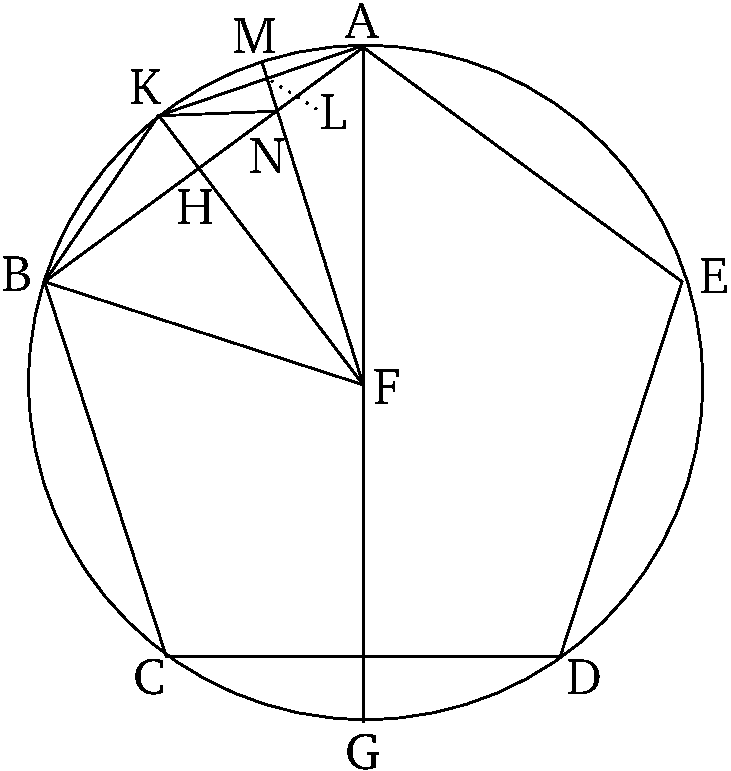
\includegraphics{Book13/fig10e.pdf}}

Let $ABCDE$ be a circle. And let the equilateral pentagon $ABCDE$
be inscribed in circle $ABCDE$. I say that the square on the
side of pentagon $ABCDE$ is the (sum of the squares) on the sides
of the hexagon and of the decagon inscribed in circle $ABCDE$. 

For let the center of the circle, point $F$, be found [Prop.~3.1]. And,
$AF$ being joined, let it be drawn across to point $G$. And
let $FB$ be joined. And let $FH$ be drawn from $F$
perpendicular to $AB$. And let it be drawn across to $K$. 
And let $AK$ and $KB$ be joined.  And, again, let $FL$ have
been drawn from $F$ perpendicular to $AK$. And let it be drawn
across to $M$. And let $KN$ be joined.

Since circumference $ABCG$ is equal to circumference $AEDG$,
of which $ABC$ is equal to $AED$, the remaining circumference
$CG$ is thus equal to the remaining (circumference) $GD$. And $CD$ (is the side) of the pentagon. 
$CG$ (is) thus (the side) of the decagon. And since  $FA$ is equal to $FB$,
and $FH$ is perpendicular (to $AB$), angle $AFK$ (is) thus also equal
to $KFB$ [Props.~1.5, 1.26]. Hence, circumference $AK$
is also equal to $KB$ [Prop.~3.26]. Thus, circumference $AB$ (is)
double circumference $BK$. Thus, straight-line $AK$ is the side of the decagon. 
So, for the same (reasons, circumference)  $AK$ is also double $KM$. And since
circumference $AB$ is double circumference $BK$, and
circumference $CD$ (is) equal to circumference $AB$, circumference
$CD$ (is) thus also double circumference $BK$. And
circumference $CD$ is also double $CG$. Thus, circumference
$CG$ (is) equal to circumference $BK$. But, $BK$
is double $KM$, since $KA$ (is) also (double $KM$). Thus,
(circumference) $CG$ is also double $KM$. But, indeed, circumference $CB$ is also
double circumference $BK$. For circumference $CB$ (is) equal to $BA$. 
Thus, the whole circumference $GB$ is also double $BM$. 
Hence, angle $GFB$ [is] also double  angle $BFM$ [Prop.~6.33].
And $GFB$ (is) also double $FAB$. For $FAB$ (is) equal to $ABF$. 
Thus, $BFN$ is also equal to $FAB$. And angle $ABF$ (is) common
to the two triangles $ABF$ and $BFN$. Thus, the
remaining (angle) $AFB$ is equal to the remaining (angle) $BNF$
[Prop.~1.32]. Thus, triangle $ABF$ is equiangular to triangle
$BFN$. Thus, proportionally, as straight-line $AB$ (is) to
$BF$, so $FB$ (is) to $BN$ [Prop.~6.4]. Thus, the (rectangle contained)
by $ABN$ is equal to the (square) on $BF$ [Prop.~6.17]. Again,
since $AL$ is equal to $LK$, and $LN$ is common and at right-angles (to $KA$), 
base $KN$ is thus equal to base $AN$  [Prop.~1.4]. And, thus, angle
$LKN$ is equal to angle $LAN$. But, $LAN$ is equal to
$KBN$ [Props.~3.29, 1.5]. Thus, $LKN$ is also equal to $KBN$. 
And the (angle) at $A$ (is) common to the two triangles $AKB$ and
$AKN$. Thus, the remaining (angle) $AKB$ is equal to the
remaining (angle) $KNA$ [Prop.~1.32]. Thus, triangle $KBA$ is
equiangular to triangle $KNA$. Thus, proportionally, as straight-line
$BA$ is to $AK$, so $KA$ (is) to $AN$ [Prop.~6.4]. Thus, the
(rectangle contained) by $BAN$ is equal to the (square) on $AK$ [Prop.~6.17]. 
And  the (rectangle contained) by $ABN$ was also shown (to be)
equal to the (square) on $BF$. Thus, the (rectangle contained) by $ABN$
plus the (rectangle contained) by $BAN$, which is the (square) on $BA$
[Prop.~2.2],
is equal to the (square) on $BF$ plus the (square) on $AK$. 
And $BA$ is the side of the pentagon, and $BF$ (the side) of the hexagon
[Prop.~4.15~corr.], and $AK$ (the side) of the decagon.

Thus, the square on the side of the pentagon  (inscribed in a circle) is (equal to) the (sum of the squares)
on the (sides) of the hexagon and of  the decagon inscribed in the
same circle.}
\end{Parallel}
{\footnotesize\noindent$^\dag$ If the circle is of unit radius then the side
of the pentagon is $(1/2)\,\sqrt{10-2\,\sqrt{5}}$.}

%%%%
%13.11
%%%%
\pdfbookmark[1]{Proposition 13.11}{pdf13.11}
\begin{Parallel}{}{}
\ParallelLText{
\begin{center}
{\large \ggn{11}.}
\end{center}\vspace*{-7pt}

\gr{Ἐὰν εἰξ κύκλον <ρητὴν >έθοντα τὴν διάμετρον πεντάγω\-νον
ἰσόπλευρον ἐγγραφῆ|, ἡ τοῦ πενταγώνου πλευρὰ >άλογόξ
ἐστιν ἡ καλουμένη ἐλάσσων.}

% Removed epsf size command
\centerline{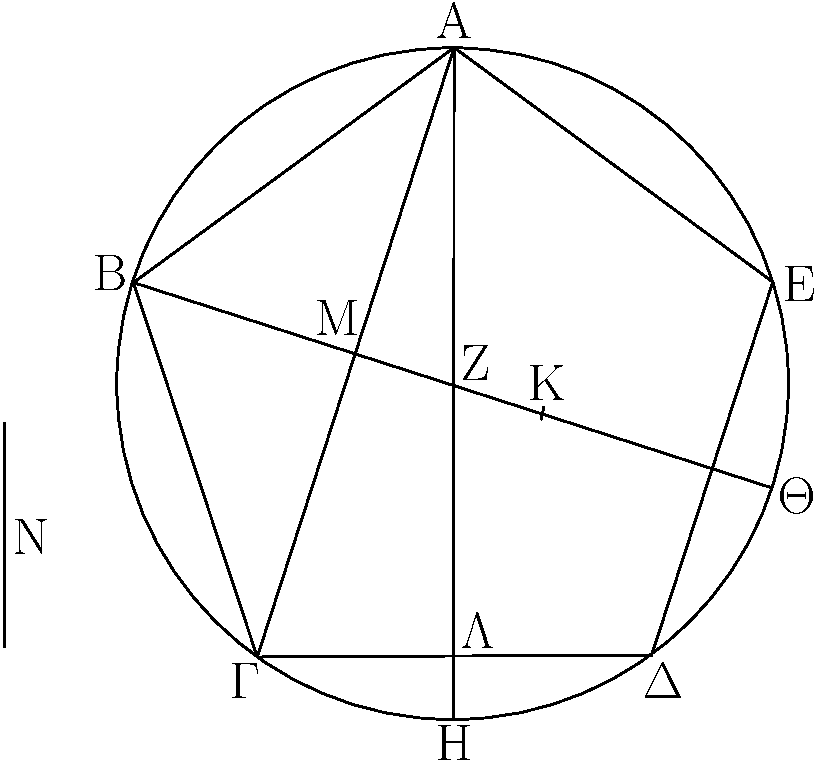
\includegraphics{Book13/fig11g.pdf}}

\gr{Εἰξ γὰρ κύκλον τὸν ΑΒΓΔΕ <ρητὴν >έθοντα τὴν δίαμετρον
πεντάγωνον ἰσόπλευρον  ἐγγεγράφθω τὸ ΑΒΓΔΕ; λέγω,
<ότι ἡ τοῦ [ΑΒΓΔΕ] πενταγώνου πλευρὰ >άλογόξ ἐστιν
ἡ καλουμένη ἐλάσσων.}

\gr{Εἰλήφθω γὰρ τὸ κέντρον τοῦ κύκλου τὸ Ζ σημεῖον, καὶ
ἐπεζεύθθωσαν αἱ ΑΖ, ΖΒ καὶ διήθθωσαν ἐπὶ τὰ Η, Θ σημεῖα,
καὶ ἐπεζεύθθω ἡ ΑΓ, καὶ κείσθω τῆξ ΑΖ τέταρτον μέροξ
ἡ ΖΚ. <ρητὴ δὲ ἡ ΑΖ; <ρητὴ >άρα καὶ ἡ ΖΚ. >έστι
δὲ καὶ ἡ ΒΖ <ρητή; <όλη >άρα ἡ ΒΚ <ρητή ἐστιν. καὶ ἐπεὶ
>ίση ἐστὶν ἡ ΑΓΗ περιφέρεια τῆ| ΑΔΗ περιφερείᾳ, <ῶν ἡ ΑΒΓ τῆ|
ΑΕΔ ἐστιν >ίση, λοιπὴ >άρα ἡ ΓΗ λοιπῆ| τῆ| ΗΔ ἐστιν >ίση.
καὶ ἒαν ἐπιζεύχωμεν τὴν ΑΔ, συνάγονται ὀρθαὶ αἱ πρὸξ τῶ|
Λ γωνίαι, καὶ διπλῆ ἡ ΓΔ τῆξ ΓΛ. διὰ τὰ α\kern -.7pt  ὐτὰ δὴ καὶ αἱ
πρὸξ τῶ| Μ ὀρθαί εἰσιν, καὶ διπλῆ ἡ ΑΓ τῆξ ΓΜ. ἐπεὶ
ο>ῦν >ίση ἐστὶν ἡ ὑπὸ ΑΛΓ γωνία τῆ| ὑπὸ ΑΜΖ, κοινὴ δὲ
τῶν δύο τριγώνων τοῦ τε ΑΓΛ καὶ τοῦ ΑΜΖ ἡ ὑπὸ ΛΑΓ,
λοιπὴ >άρα ἡ ὑπὸ ΑΓΛ λοιπῆ| τῆ| ὑπὸ ΜΖΑ ἐστιν >ίση;
ἰσογώνιον >άρα ἐστὶ τὸ ΑΓΛ τρίγωνον τῶ| ΑΜΖ τριγώνῳ;
ἀνάλογον >άρα ἐστὶν ὡξ ἡ ΛΓ πρὸξ ΓΑ, ο<ύτωξ ἡ 
ΜΖ πρὸξ ΖΑ; καὶ τῶν ἡγουμένων τὰ διπλάσια; ὡξ >άρα
ἡ τῆξ ΛΓ διπλῆ πρὸξ τὴν ΓΑ, ο<ύτωξ ἡ τῆξ ΜΖ
διπλῆ πρὸξ τὴν ΖΑ. ὡξ δὲ ἡ τῆξ ΜΖ διπλῆ πρὸξ τὴν ΖΑ,
ο<ύτωξ ἡ ΜΖ πρὸξ τὴν ἡμίσειαν τῆξ ΖΑ; καὶ ὡξ >άρα
ἡ τῆξ ΛΓ διπλῆ πρὸξ τὴν ΓΑ, ο<ύτωξ ἡ ΜΖ πρὸξ τὴν
ἡμίσειαν τῆξ ΖΑ; καὶ 
τῶν ἑπομένων τὰ ἡμίσεα; ὡξ >άρα ἡ τῆξ ΛΓ διπλῆ πρὸξ τὴν
ἡμίσειαν τῆξ ΓΑ,  ο<ύτωξ ἡ ΜΖ πρὸξ τὸ τέτατρον τῆξ ΖΑ. καί
ἐστι τῆξ μὲν ΛΓ διπλῆ ἡ ΔΓ, τῆξ δὲ ΓΑ ἡμίσεια ἡ ΓΜ,
τῆξ δὲ ΖΑ τέτατρον μέροξ ἡ ΖΚ; >έστιν >άρα ὡξ ἡ ΔΓ πρὸξ
τὴν ΓΜ, ο<ύτωξ ἡ ΜΖ πρὸξ τὴν ΖΚ. συνθέντι καὶ ὡξ συναμφότεροξ
ἡ ΔΓΜ πρὸξ τὴν ΓΜ, ο<ύτωξ ἡ ΜΚ πρὸξ ΚΖ; καὶ ὡξ >άρα
τὸ ἀπὸ συναμφοτέρου τῆξ ΔΓΜ πρὸξ τὸ ἀπὸ ΓΜ, ο<ύτωξ τὸ
ἀπὸ ΜΚ πρὸξ τὸ ἀπὸ ΚΖ. καὶ ἐπεὶ τῆξ ὑπὸ δύο
πλευρὰξ τοῦ πενταγώνου ὑποτεινούσηξ, ο<ῖον τῆξ ΑΓ, >άκρον
καὶ μέσον λόγον τεμνομένηξ τὸ μεῖζον τμ\kern -.7pt  ῆμα >ίσον ἐστὶ
τῆ| τοῦ πενταγώνου πλευρᾶ|, τουτέστι τῆ| ΔΓ, τὸ δὲ μεῖζον
τμ\kern -.5pt  ῆμα προσλαβὸν τὴν ἡμίσειαν τῆξ <όλῆξ πενταπλάσιον
δύναται τοῦ ἀπὸ τῆξ ἡμισείαξ τῆξ <όληξ, καί ἐστιν <όληξ τῆξ
ΑΓ ἡμίσεια ἡ ΓΜ, τὸ >άρα ἀπὸ τῆξ ΔΓΜ ὡξ μιᾶξ
πενταπλάσιόν ἐστι τοῦ ἀπὸ τῆξ ΓΜ. ὡξ δὲ τὸ ἀπὸ τῆξ
ΔΓΜ ὡξ μιᾶξ πρὸξ τὸ ἀπὸ τῆξ ΓΜ, ο<ύτωξ ἐδείθθη τὸ
ἀπὸ τῆξ ΜΚ πρὸξ τὸ ἀπὸ τῆξ ΚΖ; πενταπλάσιον >άρα τὸ ἀπὸ
τῆξ ΜΚ τοῦ ἀπὸ τῆξ ΚΖ. <ρητὸν δὲ τὸ ἀπὸ τῆξ ΚΖ;
<ρητὴ γὰρ ἡ  διάμετροξ; <ρητὸν >άρα καὶ τὸ ἀπὸ τῆξ ΜΚ;
<ρητὴ >άρα  ἐστὶν ἡ ΜΚ [δυνάμει μόνον]. καὶ ἐπεὶ
τετραπλασία ἐστὶν ἡ ΒΖ τῆξ ΖΚ, πενταπλασία >άρα ἐστὶν
ἡ ΒΚ τῆξ  ΚΖ;
εἰκοσιπενταπλάσιον >άρα τὸ ἀπὸ τῆξ ΒΚ τοῦ ἀπὸ τῆξ ΚΖ.
πενταπλάσιον δὲ τὸ ἀπὸ τῆξ ΜΚ τοῦ ἀπὸ τῆξ ΚΖ; πενταπλάσιον
>άρα τὸ ἀπὸ τῆξ ΒΚ τοῦ ἀπὸ τῆξ ΚΜ; τὸ >άρα ἀπὸ τῆξ
ΒΚ πρὸξ τὸ ἀπὸ ΚΜ λόγον οὐκ >έθει, <ὸν τετράγωνοξ ἀριθμὸξ
πρὸξ τετράγωνον ἀριθμόν; ἀσύμμετροξ >άρα ἐστὶν ἡ ΒΚ τῆ| ΚΜ
μ\kern -.3pt  ήκει. καί ἐστι <ρητὴ ἑκατέρα α\kern -.7pt  ὐτῶν. αἱ ΒΚ, ΚΜ >άρα
<ρηταί εἰσι δυνάμει μόνον σύμμετροι. ἒαν δὲ ἀπὸ <ρητῆξ
<ρητὴ ἀφαιρεθῆ| δυνάμει μόνον σύμμετροξ ο>ῦσα τῆ|
<όλῃ, ἡ λοιπὴ >άλογόξ ἐστιν ἀποτομ\kern -.7pt  ή; ἀποτομ\kern -.7pt  ὴ >άρα
ἐστὶν ἡ ΜΒ, προσαρμόζουσα δὲ α\kern -.7pt  ὐτῆ| ἡ ΜΚ. λέγω δή,
<ότι καὶ τετάρτη. <ῶ| δὴ μεῖζόν ἐστι τὸ ἀπὸ τῆξ ΒΚ
τοῦ ἀπὸ τῆξ ΚΜ, ἐκείνῳ >ίσον >έστω τὸ ἀπὸ τῆξ
Ν; ἡ ΒΚ >άρα τῆξ ΚΜ
μεῖζον δύναται τῆ| Ν. καὶ ἐπεὶ
σύμμετρόξ ἐστιν ἡ ΚΖ τῆ| ΖΒ, καὶ συνθέντι σύμμετρόξ ἐστι ἡ ΚΒ τῆ| ΖΒ. ἀλλὰ ἡ ΒΖ τῆ| ΒΘ σύμμετρόξ ἐστιν; καὶ ἡ ΒΚ >άρα τῆ|
ΒΘ σύμμετρόξ ἐστιν. καὶ ἐπεὶ πενταπλάσιόν ἐστι τὸ ἀπὸ τῆξ
ΒΚ τοῦ ἀπὸ τῆξ ΚΜ, τὸ >άρα ἀπὸ τῆξ ΒΚ πρὸξ τὸ ἀπὸ
τῆξ ΚΜ λόγον >έθει, <ὸν \kern -.7pt {ε} pr`oc <'en. >anastr'eyanti >'ara
t`o >ap`o t~hc BK pr`oc t`o >ap`o t~hc N l'ogon >'eqei, <`on \ov{e}
pr`oc \ov{d}, o>uq <`on tetr'agwnoc pr`oc tetr'agwnon; >as'ummetroc
>'ara >est`in <h BK t~h| N; <h BK >'ara t~hc KM me~izon
d'unatai t~w| >ap`o >asumm'etrou <eaut~h|. >epe`i o>~un <'olh
<h BK t~hc prosarmozo'ushc t~hc KM me~izon d'unatai t~w| >ap`o
>asumm'etrou <eaut~h|, ka`i <'olh <h BK s'ummetr'oc >esti t~h| >ekkeim'enh|
<rht~h| t~h| BJ, >apotom\kern -.7pt `h >'ara tet'arth >est`in <h MB. t`o d`e <up`o <rht~hc
ka`i >apotom\kern -.7pt ~hc tet'arthc perieq'omenon >orjog'wnion >'alog'on >estin,
ka`i <h dunam'enh a\kern -.7pt >ut`o >'alog'oc >estin, kale~itai d`e >el'attwn. d'unatai
d`e t`o <up`o t~wn JBM <h AB di`a t`o >epizeugnum'enhc
t~hc AJ >isog'wnion g'inesjai t`o ABJ tr'igwnon t~w| ABM trig'wnw|
ka`i e>~inai <wc t`hn JB pr`oc t`hn BA, o<'utwc t`hn AB pr`oc
t`hn BM.}

\gr{Ἡ >άρα ΑΒ τοῦ πενταγώνου πλευρὰ >άλογόξ ἐστιν ἡ καλουμένη
ἐλάττων; <όπερ >έδει δεῖχαι.}}

\ParallelRText{
\begin{center}
{\large Proposition 11}
\end{center}

If an equilateral pentagon is inscribed in a circle which has a rational  diameter  then the side of the pentagon is that irrational
(straight-line) called minor.

% Removed epsf size command
\centerline{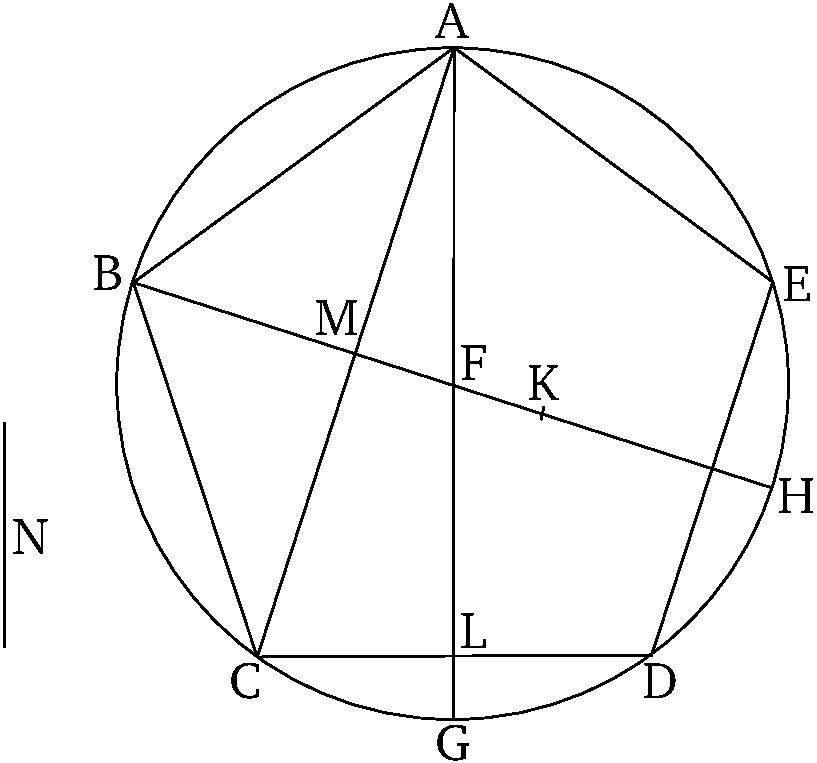
\includegraphics{Book13/fig11e.pdf}}

For let the equilateral pentagon $ABCDE$ be inscribed  in the circle $ABCDE$ which has a rational diameter. I say that the side of pentagon
[$ABCDE$] is that irrational (straight-line) called minor.

For let the center of the circle, point $F$, be found [Prop.~3.1].
And let $AF$ and $FB$ be joined. And let them be drawn
across to points $G$ and $H$ (respectively). And let $AC$ be joined.
And let $FK$ made (equal) to the fourth part of $AF$. And $AF$ (is) rational. $FK$ (is) thus also rational. And $BF$ is also rational. Thus,
the whole of $BK$ is rational. And since circumference $ACG$ is equal
to circumference $ADG$, of which $ABC$ is equal to $AED$, the
remainder $CG$ is thus equal to the remainder $GD$.
And if we join $AD$ then the angles at $L$ are inferred (to be) right-angles, 
and $CD$ (is inferred to be) double $CL$ [Prop.~1.4].  So, for the same (reasons), 
the (angles) at $M$ are also right-angles, and $AC$ (is) double $CM$. Therefore,
since angle $ALC$ (is) equal to $AMF$, and (angle) $LAC$ (is) common
to the two triangles $ACL$ and $AMF$, the remaining (angle) $ACL$ is thus
equal to the remaining (angle) $MFA$ [Prop.~1.32]. Thus, triangle 
$ACL$  is equiangular to triangle $AMF$. Thus, proportionally, 
as $LC$ (is) to $CA$, so $MF$ (is) to $FA$ [Prop.~6.4]. And (we can take) the
doubles of the leading (magnitudes). Thus, as double $LC$ (is) to $CA$,
so double $MF$ (is) to $FA$. And as double $MF$ (is) to $FA$, so
$MF$ (is) to half of $FA$. And, thus, as double $LC$ (is) to $CA$,
so $MF$ (is) to half of $FA$. And (we can take) the halves of the following
(magnitudes). Thus, as double $LC$ (is) to half of $CA$, so $MF$
(is) to the fourth of $FA$. And $DC$ is double $LC$, and  $CM$ half
of $CA$, and $FK$ the fourth part of $FA$.  Thus, as $DC$
is to $CM$, so $MF$ (is) to $FK$. Via composition, as the
sum of $DCM$ ({\em i.e.}, $DC$ and $CM$)
(is) to $CM$, so $MK$ (is) to $KF$ [Prop.~5.18]. And, thus, as the (square) on the
sum of $DCM$ (is) to the (square) on $CM$, so the (square) on $MK$
(is) to the (square) on $KF$. And since the
greater piece of a (straight-line) subtending two sides of a
pentagon, such as $AC$, (which is) cut in extreme and mean ratio is equal to the side of the pentagon [Prop.~13.8]---that is to say,
to $DC$----and the square on the greater piece added to half of the
whole is five times the (square) on half of the whole [Prop.~13.1], 
and $CM$ (is) half of the whole, $AC$, thus the (square) on
$DCM$, (taken) as one, is five times the (square) on $CM$.
And the (square) on $DCM$, (taken) as one,  (is)  to the (square) on $CM$, so the (square) on $MK$ was shown (to be) to the (square) on 
$KF$.  Thus, the (square) on $MK$ (is) five times the (square) on 
$KF$. And the square on $KF$ (is) rational. For the diameter
(is) rational. Thus, the (square) on $MK$ (is) also rational. 
Thus, $MK$ is rational [in square only]. And since $BF$ is four times
$FK$, $BK$ is thus five times $KF$. Thus, the (square) on $BK$
(is) twenty-five times the (square) on $KF$.  And the (square) on $MK$
(is) five times the square on $KF$. Thus, the (square) on $BK$ (is) five
times the (square) on $KM$.  Thus, the (square) on $BK$ does not
have to the (square) on $KM$ the ratio which a square number (has) to
a square number. Thus, $BK$ is incommensurable in length with $KM$ [Prop.~10.9].
And each of them is a rational (straight-line).  Thus, $BK$ and $KM$ are rational
(straight-lines which are) commensurable in square only. And if from a rational (straight-line)
a rational (straight-line) is subtracted, which is commensurable in square
only with the whole, then the remainder is that irrational (straight-line
called) an apotome [Prop.~10.73]. Thus, $MB$ is an apotome, and $MK$ its attachment. So, I say that (it is) also a fourth (apotome). So, let the
(square) on $N$ be (made) equal to that (magnitude) by which the (square)
on $BK$ is greater than the (square) on $KM$. Thus, the
square on $BK$ is greater than the (square) on $KM$ by the (square) on $N$.
And since $KF$ is commensurable (in length) with $FB$ then, via composition, 
$KB$ is also commensurable (in length) with $FB$ [Prop.~10.15]. But, $BF$ is commensurable (in length)
with $BH$. Thus, $BK$ is also commensurable (in length) with $BH$ [Prop.~10.12]. And since the
(square) on $BK$ is five times the (square) on $KM$, the (square) on $BK$
thus has to the (square) on $KM$ the ratio which 5 (has) to one. Thus, via
conversion, the (square) on $BK$ has to the (square) on $N$ the ratio
which 5 (has) to 4 [Prop.~5.19~corr.], which is not (that) of a
square (number) to a square (number). $BK$ is thus incommensurable (in length)
with $N$ [Prop.~10.9]. Thus, the square on $BK$ is greater than
the (square) on $KM$ by the (square) on (some straight-line which is) incommensurable (in length) with ($BK$). Therefore, since the square on the whole,
$BK$, is greater than the (square) on the attachment, $KM$, by the
(square) on (some straight-line which is) incommensurable (in length) with ($BK$),
and the whole, $BK$, is commensurable (in length) with the (previously) laid down
rational (straight-line) $BH$, $MB$ is thus a fourth apotome
[Def.~10.14]. And the rectangle contained by a rational (straight-line)
and a fourth apotome is irrational, and its square-root is that irrational
(straight-line) called minor [Prop.~10.94]. And the square on $AB$
is the rectangle contained by $HBM$, on account of joining $AH$, (so that)
triangle $ABH$ becomes equiangular  with triangle $ABM$ [Prop.~6.8], and (proportionally) as
$HB$ is to $BA$, so $AB$ (is) to $BM$.

Thus, the side $AB$ of the pentagon is that irrational (straight-line)
called minor.$^\dag$ (Which is) the very thing it was required to show.}
\end{Parallel}
{\footnotesize\noindent$^\dag$ If the circle has unit radius then the side of the pentagon is $(1/2)\,\sqrt{10-2\,\sqrt{5}}$. However, this length can
be written in the ``minor'' form (see Prop.~10.94) $(\rho/\sqrt{2})\,\sqrt{1+k/\sqrt{1+k^2}} - (\rho/\sqrt{2})\,\sqrt{1-k/\sqrt{1+k^2}}$, with $\rho=\sqrt{5/2}$ and $k=2$.}

%%%%
%13.12
%%%%
\pdfbookmark[1]{Proposition 13.12}{pdf13.12}
\begin{Parallel}{}{}
\ParallelLText{
\begin{center}
{\large \ggn{12}.}
\end{center}\vspace*{-7pt}

\gr{Ἐὰν εἰξ κύκλον τρίγωνον ἰσόπλευρον ἐγγραφῆ|, ἡ τοῦ
τριγώνου πλευρὰ δυνάμει τριπλασίων ἐστὶ τῆξ ἐκ τοῦ
κέντρου τοῦ κύκλου.}

\gr{Ἐστω κύκλοξ ὁ ΑΒΓ, καὶ εἰξ α\kern -.7pt  ὐτὸν τρίγωνον ἰσόπλευρ\-ον
ἐγγεγράφθω τὸ ΑΒΓ; λέγω, <ότι τοῦ ΑΒΓ τριγώνου μία πλευρὰ
δυνάμει τριπλασίων ἐστὶ τῆξ ἐκ τοῦ κέντρου τοῦ ΑΒΓ κύκλου.}

% Removed epsf size command
\centerline{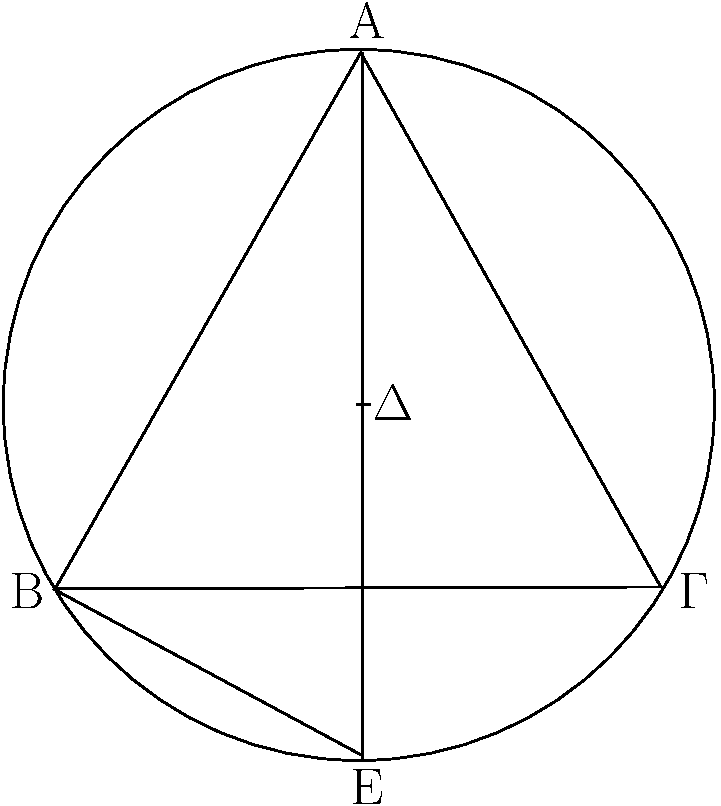
\includegraphics{Book13/fig12g.pdf}}

\gr{ Εἰλήφθω γὰρ τὸ κέντρον τοῦ ΑΒΓ κύκλου τὸ Δ, καὶ
ἐπιζευθθεῖσα ἡ ΑΔ διήθθω ἐπὶ τὸ Ε, καὶ ἐπεζεύθθω ἡ ΒΕ.}

\gr{Καὶ ἐπεὶ ἰσόπλευρόν
ἐστι τὸ ΑΒΓ τρίγωνον, ἡ ΒΕΓ >άρα περιφέρεια τρίτον
μέροξ ἐστὶ τῆξ τοῦ ΑΒΓ κύκλου περιφερείαξ. ἡ >άρα ΒΕ
περιφέρεια <έκτον ἐστὶ μέροξ τῆξ τοῦ κύκλου περιφερείαξ;
ἑχαγώνου >άρα ἐστὶν ἡ ΒΕ εὐθεῖα; >ίση >άρα ἐστὶ τῆ|
ἐκ τοῦ κέντρου τῆ| ΔΕ. καὶ ἐπεὶ διπλῆ ἐστιν ἡ ΑΕ
τῆξ ΔΕ, τετραπλάσιον ἐστι τὸ ἀπὸ τῆξ ΑΕ τοῦ ἀπὸ
τῆξ ΕΔ, τουτέστι τοῦ ἀπὸ τῆξ ΒΕ. >ίσον δὲ τὸ ἀπὸ
τῆξ ΑΕ τοῖξ ἀπὸ τῶν ΑΒ, ΒΕ; τὰ >άρα ἀπὸ τῶν ΑΒ, ΒΕ
τετραπλάσιά ἐστι τοῦ ἀπὸ τῆξ ΒΕ. διελόντι >άρα τὸ ἀπὸ
τῆξ ΑΒ τριπλάσιόν ἐστι τοῦ ἀπὸ ΒΕ. >ίση δὲ ἡ ΒΕ τῆ| ΔΕ;
τὸ >άρα ἀπὸ τῆξ ΑΒ τριπλάσιόν ἐστι τοῦ ἀπὸ τῆξ ΔΕ.}

\gr{Ἡ >άρα τοῦ τριγώνου πλευρὰ δυνάμει τριπλασία
ἐστὶ τῆξ ἐκ τοῦ κέντρου [τοῦ κύκλου]; <όπερ >έδει
δεῖχαι.}}

\ParallelRText{
\begin{center}
{\large Proposition 12}
\end{center}

If an equilateral triangle is inscribed in a circle then the
square on the side of the triangle is three times the (square) on
the radius of the circle.

Let there be a circle $ABC$, and let the equilateral triangle $ABC$ have
been inscribed in it  [Prop.~4.2]. I say that the square on one side of triangle
$ABC$ is three times the (square) on the radius of circle $ABC$. 

% Removed epsf size command
\centerline{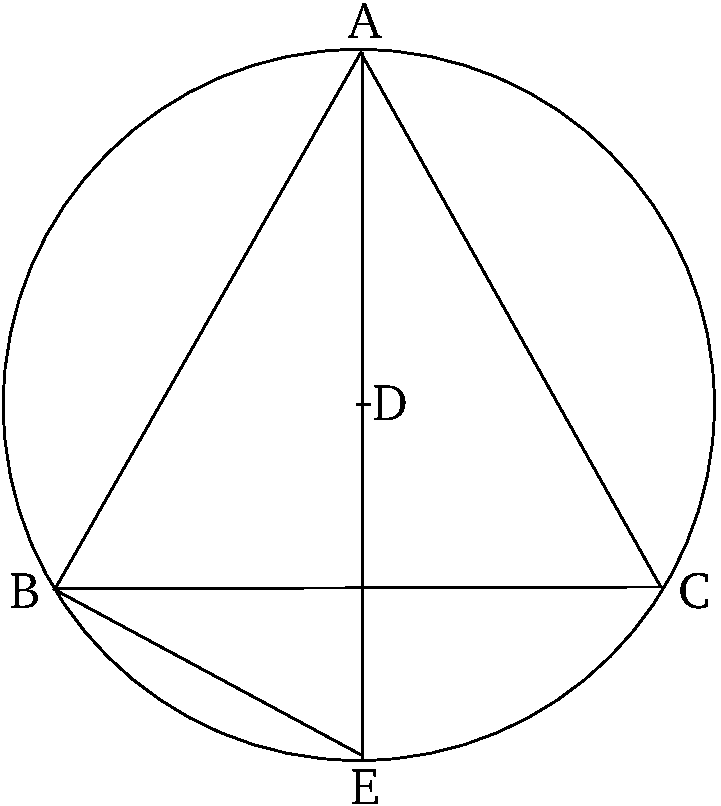
\includegraphics{Book13/fig12e.pdf}}

For let the center, $D$, of circle $ABC$ be found [Prop.~3.1].
And  $AD$ (being) joined, let it be drawn across to $E$. 
And let $BE$ be joined.

And since triangle $ABC$ is equilateral, circumference $BEC$ is thus the
third part of the circumference of circle $ABC$. Thus, 
circumference $BE$ is the sixth part of the circumference of the circle. 
Thus, straight-line $BE$ is (the side) of a hexagon. Thus, it is equal to the radius
$DE$ [Prop.~4.15~corr.]. And since $AE$ is double $DE$, the (square)
on $AE$ is four times the (square) on $ED$---that is to say, of the
(square) on $BE$.  And the (square) on $AE$ (is) equal to
the (sum of the squares) on $AB$ and $BE$ [Props.~3.31, 1.47]. 
Thus, the (sum of the squares) on $AB$ and $BE$ is four times the
(square) on $BE$. Thus, via separation, the (square) on $AB$ is three
times the (square) on $BE$. And $BE$ (is) equal to $DE$. Thus, the
(square) on $AB$ is three times the (square) on $DE$.

Thus, the square on the side of the triangle is three times the (square)
on the radius [of the circle]. (Which is) the very thing it was required to show.}
\end{Parallel}

%%%%
%13.13
%%%%
\pdfbookmark[1]{Proposition 13.13}{pdf13.13}
\begin{Parallel}{}{}
\ParallelLText{
\begin{center}
{\large \ggn{13}.}
\end{center}\vspace*{-7pt}

\gr{Πυραμίδα συστήσασθαι καὶ σφαίρᾳ περιλαβεῖν τῆ| δοθείσῃ καὶ
δεῖχαι, <ότι ἡ τῆξ σφαίραξ διάμετροξ δυνάμει ἡμιολία ἐστὶ
τῆξ πλευρᾶξ τῆξ πυραμίδοξ.}

\gr{Ἐκκείσθω ἡ τῆξ δοθείσηξ σφαίραξ δίαμετροξ ἡ ΑΒ, καὶ
τετμ\kern -.7pt  ήσθω κατὰ τὸ Γ σημεῖον, <ώστε διπλασίαν ε>ῖναι τὴν
ΑΓ τῆξ ΓΒ; καὶ γεγράφθω ἐπὶ τῆξ ΑΒ ἡμικύκλιον τὸ
ΑΔΒ, καὶ >ήθθω ἀπὸ τοῦ Γ σημείου τῆ| ΑΒ πρὸξ ὀρθὰξ
ἡ ΓΔ, καὶ ἐπεζεύθθω ἡ ΔΑ; καὶ ἐκκείσθω κύκλοξ
ὁ ΕΖΗ >ίσην >έθων τὴν ἐκ τοῦ κέντρου τῆ| ΔΓ, καὶ
ἐγγεγράφθω εἰξ τὸν ΕΖΗ κύκλον τρίγωνον ἰσόπλευρον
τὸ ΕΖΗ; καὶ εἰλήφθω τὸ κέντρον τοῦ κύκλου τὸ Θ σημεῖον,
καὶ ἐπεζεύθθωσαν αἱ ΕΘ, ΘΖ, ΘΗ; καὶ ἀνεστάτω ἀπὸ τοῦ
Θ σημείου τῶ| τοῦ ΕΖΗ κύκλου ἐπιπέδῳ πρὸξ ὀρθὰξ
ἡ ΘΚ, καὶ ἀφῃρήσθω ἀπὸ τῆξ ΘΚ τῆ| ΑΓ εὐθείᾳ
>ίση ἡ ΘΚ, καὶ ἐπεζεύθθωσαν αἱ ΚΕ, ΚΖ, ΚΗ. καὶ
ἐπεὶ ἡ ΚΘ ὀρθή ἐστι πρὸξ τὸ τοῦ ΕΖΗ κύκλου ἐπίπεδον,
καὶ πρὸξ πάσαξ >άρα τὰξ ἁπτομέναξ α\kern -.7pt  ὐτῆξ εὐθείαξ
καὶ ο>ύσαξ ἐν τῶ| τοῦ ΕΖΗ κύκλου ἐπιπέδῳ
ὀρθὰξ ποιήσει γωνίαξ. <άπτεται δὲ α\kern -.5pt  ὐτῆξ ἑκάστη
τῶν ΘΕ, ΘΖ, ΘΗ; ἡ ΘΚ >άρα πρὸξ ἑκάστη τῶν ΘΕ, ΘΖ,
ΘΗ
 ὀρθή ἐστιν. καὶ ἐπεὶ >ίση ἐστὶν ἡ μὲν
ΑΓ τῆ| ΘΚ, ἡ δὲ ΓΔ τῆ| ΘΕ, καὶ ὀρθὰξ γωνίαξ περιέθουσιν,
βάσιξ >άρα ἡ ΔΑ βάσει τῆ| ΚΕ ἐστιν >ίση. διὰ τὰ α\kern -.3pt  ὐτὰ
δὴ καὶ ἑκατέρα τῶν ΚΖ, ΚΗ τῆ| ΔΑ ἐστιν >ίση;
αἱ τρεῖξ >άρα αἱ ΚΕ, ΚΖ, ΚΗ >ίσαι ἀλλήλαιξ εἰσίν.
καὶ ἐπεὶ διπλῆ ἐστιν ἡ ΑΓ τῆξ ΓΒ, τριπλῆ >άρα ἡ
ΑΒ τῆξ ΒΓ. ὡξ δὲ ἡ ΑΒ πρὸξ τὴν ΒΓ, ο<ύτωξ τὸ ἀπὸ
τῆξ ΑΔ πρὸξ τὸ ἀπὸ τῆξ ΔΓ, ὡξ ἑχῆξ δειθθήσεται.
τριπλάσιον >άρα τὸ ἀπὸ τῆξ ΑΔ τοῦ ἀπὸ τῆξ
ΔΓ. >έστι δὲ καὶ τὸ ἀπὸ τῆξ ΖΕ τοῦ ἀπὸ τῆξ ΕΘ τριπλάσιον,
καί ἐστιν >ίση ἡ ΔΓ τῆ| ΕΘ; >ίση >άρα καὶ ἡ ΔΑ τῆ| ΕΖ.
ἀλλὰ ἡ ΔΑ ἑκάστῃ τῶν ΚΕ, ΚΖ, ΚΗ ἐδείθθη >ίση;
καὶ ἑκάστη >άρα τῶν ΕΖ, ΖΗ, ΗΕ ἑκάστῃ τῶν ΚΕ, ΚΖ, ΚΗ
ἐστιν >ίση; ἰσόπλευρα >άρα ἐστὶ τὰ τέσσαρα τρίγωνα τὰ ΕΖΗ, ΚΕΖ,
ΚΖΗ, ΚΕΗ. πυραμὶξ >άρα συνέσταται ἐκ τεσσάρων τριγώνων
ἰσοπλέυρων, <ῆξ βάσιξ μέν ἐστι τὸ ΕΖΗ τρίγωνον,
κορυφὴ δὲ τὸ Κ σημεῖον.}\\~\\~\\

% Removed epsf size command
\centerline{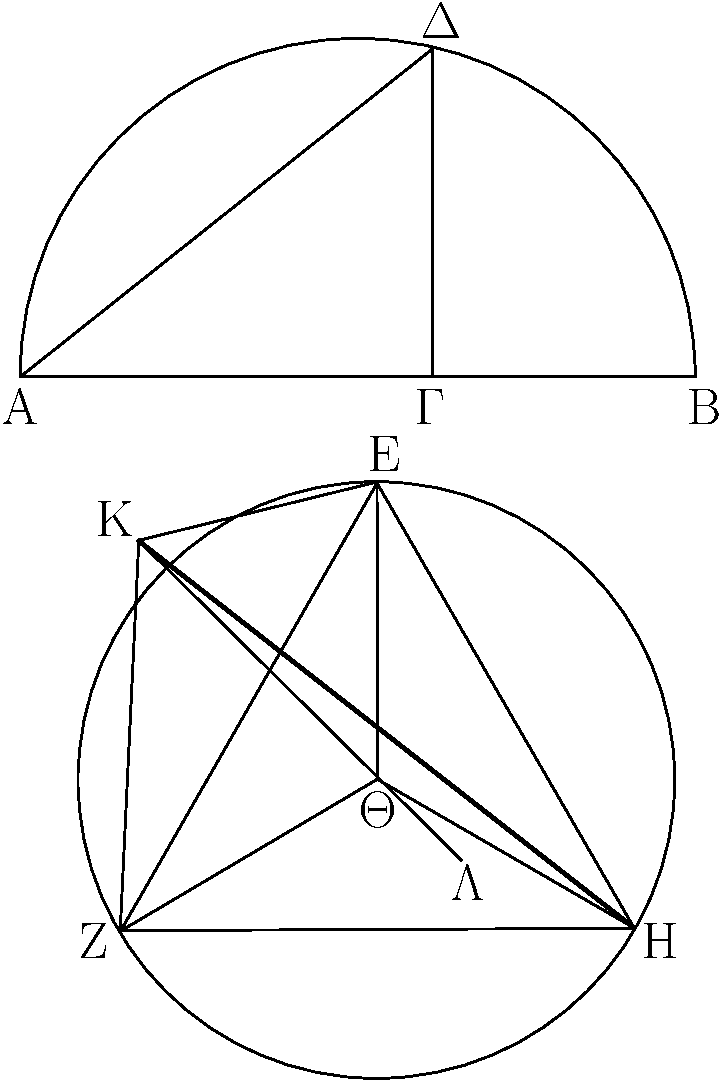
\includegraphics{Book13/fig13g.pdf}}

\gr{Δεῖ δὴ α\kern -.7pt  ὐτὴν καὶ σφαίρᾳ περιλαβεῖν τῆ| δοθείσῃ καὶ δεῖχαι,
<ότι ἡ τῆξ σφαίραξ διάμετροξ ἡμιολία ἐστὶ δυνάμει τῆξ
πλευρᾶξ τῆξ πυραμίδοξ.}

\gr{Ἐκβεβλήσθω γὰρ ἐπ> εὐθείαξ τῆ| ΚΘ εὐθεῖα ἡ ΘΛ, καὶ
κείσθω τῆ| ΓΒ >ίση ἡ ΘΛ. καὶ ἐπεί ἐστιν ὡξ ἡ ΑΓ πρὸξ
τὴν ΓΔ, ο<ύτωξ ἡ ΓΔ πρὸξ τὴν ΓΒ, >ίση δὲ ἡ μὲν ΑΓ τῆ|
ΚΘ, ἡ δὲ ΓΔ τῆ| ΘΕ, ἡ δὲ ΓΒ τῆ| ΘΛ, >έστιν >άρα ὡξ ἡ ΚΘ πρὸξ
τὴν ΘΕ, ο<ύτωξ ἡ ΕΘ πρὸξ τὴν ΘΛ; τὸ >άρα ὑπὸ τῶν
ΚΘ, ΘΛ >ίσον ἐστὶ τῶ| ἀπὸ τῆξ ΕΘ. καί ἐστιν ὀρθὴ ἑκατέρα
τῶν ὑπὸ ΚΘΕ, ΕΘΛ γωνιῶν; τὸ >άρα ἐπὶ τῆξ ΚΛ γραφόμενον
ἡμικύκλιον <ήχει καὶ διὰ τοῦ Ε [ἐπειδήπερ ἒαν ἐπιζεύχωμεν
τὴν ΕΛ, ὀρθὴ γίνεται ἡ ὑπὸ ΛΕΚ γωνία διὰ τὸ ἰσογώνιον
γίνεσθαι τὸ ΕΛΚ τρίγωνον ἑκατέρῳ τῶν ΕΛΘ, ΕΘΚ τριγώνων].
ἒαν δὴ μενούσηξ τῆξ ΚΛ περιενεθθὲν τὸ ἡμικύκλιον
εἰξ τὸ α\kern -.7pt  ὐτὸ πάλιν ἀποκατασταθῆ|, <όθεν >ήρχατο φέρεσθαι,
<ήχει καὶ διὰ τῶν Ζ, Η σημείων ἐπιζευγνυμένων
τῶν ΖΛ, ΛΗ καὶ ὀρθῶν ὁμοίωξ γινομένων τῶν πρὸξ τοῖξ
Ζ, Η γωνιῶν; καὶ >έσται ἡ πυραμὶξ σφαίρᾳ περιειλημμένη τῆ|
δοθείσῆ|. ἡ γὰρ ΚΛ τῆξ σφαίραξ διάμετροξ >ίση ἐστὶ τῆ|
τῆξ δοθείσηξ σφαίραξ διαμετρῳ τῆ| ΑΒ, ἐπειδήπερ τῆ| μὲν
ΑΓ >ίση κεῖται ἡ ΚΘ, τῆ| δὲ ΓΒ ἡ ΘΛ.}

\gr{Λέγω δή, <ότι ἡ τῆξ σφαίραξ διάμετροξ ἡμιολία
ἐστὶ δυνάμει τῆξ πλευρᾶξ τῆξ πυραμίδοξ.}

\gr{Ἐπεὶ γὰρ διπλῆ ἐστιν ἡ ΑΓ τῆξ ΓΒ, τριπλῆ >άρα
ἐστὶν ἡ ΑΒ τῆξ ΒΓ; ἀναστρέψαντι ἡμιολία >άρα ἐστὶν
ἡ ΒΑ τῆξ
ΑΓ. ὡξ δὲ ἡ ΒΑ πρὸξ τὴν ΑΓ, ο<ύτωξ
τὸ ἀπὸ τῆξ ΒΑ πρὸξ τὸ ἀπὸ τῆξ ΑΔ [ἐπειδήπερ ἐπιζευγνμένηξ
τῆξ ΔΒ ἐστιν ὡξ ἡ ΒΑ πρὸξ τὴν ΑΔ, ο<ύτωξ ἡ ΔΑ πρὸξ
τὴν ΑΓ διὰ τὴν ὁμοιότητα τῶν ΔΑΒ, ΔΑΓ τριγώνων, καὶ
ε>ῖναι ὡξ τὴν πρώτην πρὸξ τὴν τρίτην, ο<ύτωξ
τὸ ἀπὸ τῆξ τρώτηξ πρὸξ τὸ ἀπὸ τῆξ δευτέραξ].
ἡμιόλιον >άρα καὶ τὸ ἀπὸ τῆξ ΒΑ τοῦ ἀπὸ τῆξ ΑΔ. καί
ἐστιν ἡ μὲν ΒΑ ἡ τῆξ δοθείσηξ
σφαίραξ διάμετροξ, ἡ δὲ ΑΔ >ίση τῆ| πλευρᾶ|
τῆξ πυραμίδοξ.}

\gr{Ἡ >άρα τῆξ σφαίραξ διάμετροξ ἡμιολία ἐστὶ τῆξ
πλευρᾶξ τῆξ πυραμίδοξ; <όπερ >έδει δεῖχαι.}}

\ParallelRText{
\begin{center}
{\large Proposition 13}
\end{center}

To construct a (regular) pyramid ({\em i.e.}, a tetrahedron), and to
enclose (it) in a given sphere, and to show that the square on the
diameter of the sphere is one and a half times the (square) on the side 
of the pyramid. 

Let the diameter $AB$ of the given sphere be laid out, and let it be
cut at point $C$ such that $AC$ is double $CB$ [Prop.~6.10]. And let the semi-circle 
$ADB$  be drawn on $AB$. And let $CD$ be drawn from point
$C$ at right-angles to $AB$. And let $DA$ be joined. 
And let the circle $EFG$ be laid down having a radius equal to $DC$,
and let the equilateral triangle $EFG$ be inscribed in circle
$EFG$ [Prop.~4.2]. And let the center of the circle, point $H$,
be found [Prop.~3.1]. And let $EH$, $HF$, and $HG$ be
joined. And let $HK$ be set up, at point $H$, at right-angles to the
plane of circle $EFG$ [Prop.~11.12]. And let $HK$, equal to the straight-line $AC$, be cut off from $HK$. And let $KE$, $KF$, and $KG$ be joined.
And since $KH$ is at right-angles to the plane of circle $EFG$, it will
thus also make right-angles with all of the straight-lines joining it
(which are) also in the plane of circle $EFG$ [Def.~11.3]. And $HE$, $HF$,
and $HG$ each join it. Thus, $HK$ is at right-angles to each of $HE$,
$HF$, and $HG$. And since  $AC$ is equal to $HK$, and $CD$ to
$HE$, and they contain right-angles, the base $DA$ is thus equal to the base 
$KE$ [Prop.~1.4]. So, for the same (reasons),  $KF$ and
$KG$ is each equal to $DA$. Thus, the three (straight-lines)
$KE$, $KF$, and $KG$ are equal to one another. And since 
$AC$ is double $CB$, $AB$ (is) thus triple $BC$. And as 
$AB$ (is) to $BC$, so the (square) on $AD$ (is) to the (square)
on $DC$, as will be shown later [see lemma]. Thus, the (square)
on $AD$ (is) three times the (square) on $DC$. And the (square)
on $FE$ is also three times the (square) on $EH$ [Prop.~13.12], 
and $DC$ is equal to $EH$. Thus, $DA$ (is) also equal to $EF$.
But, $DA$ was shown (to be) equal to each of $KE$, $KF$, and
$KG$. Thus, $EF$, $FG$, and $GE$ are equal to 
$KE$, $KF$, and $KG$, respectively. Thus, the four triangles $EFG$, $KEF$,
$KFG$, and $KEG$ are equilateral. Thus, a pyramid, whose base is triangle
$EFG$, and apex the point $K$,   has been
constructed from four equilateral triangles.

% Removed epsf size command
\centerline{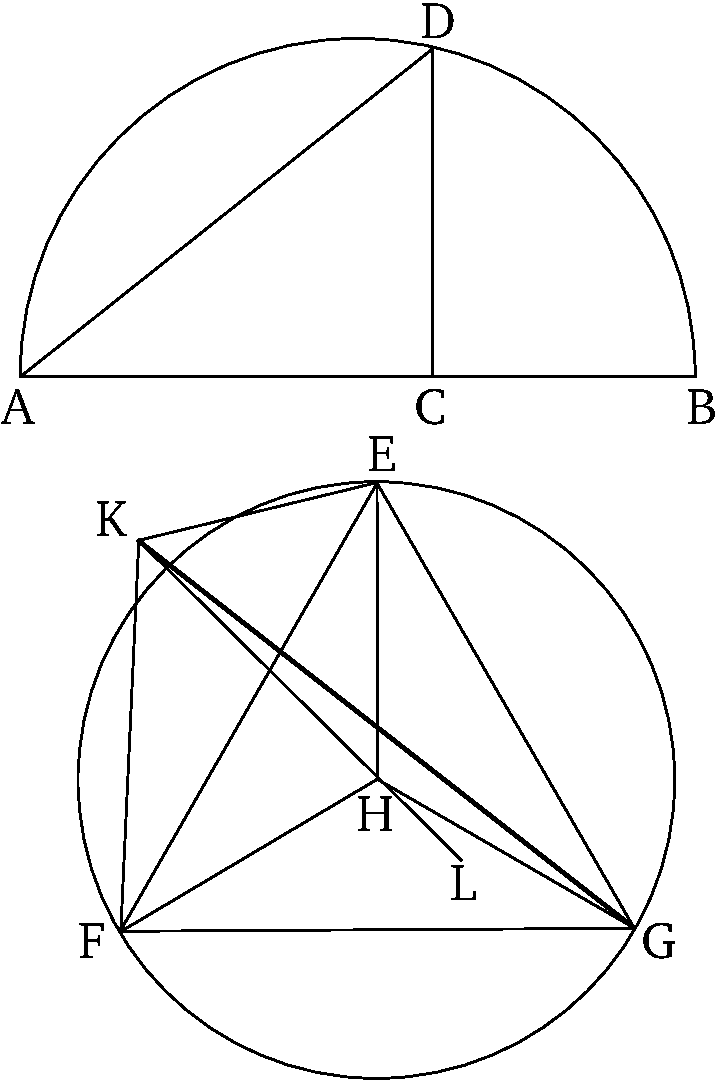
\includegraphics{Book13/fig13e.pdf}}

So, it is also necessary to enclose it in the given sphere, and to show that
the square on the diameter of the sphere is one and a half times the (square)
on the side of the pyramid. 

For let the straight-line $HL$ be produced in a straight-line with $KH$, and let
$HL$ be made equal to $CB$. And since as $AC$ (is) to $CD$, 
so $CD$ (is) to $CB$ [Prop.~6.8~corr.], and $AC$ (is) equal to $KH$, and $CD$ to
$HE$, and $CB$ to $HL$, thus as $KH$ is to $HE$, so $EH$ (is) to $HL$.
Thus,  the (rectangle contained) by $KH$ and $HL$ is equal to the
(square) on $EH$ [Prop.~6.17]. And each of the angles $KHE$ and
$EHL$ is a right-angle. Thus, the semi-circle drawn on $KL$ 
will also pass through $E$ [inasmuch as if we join $EL$ then the angle
$LEK$ becomes a right-angle, on account of triangle $ELK$
becoming equiangular to each of the triangles $ELH$ and $EHK$ [Props.~6.8, 3.31]\,]. So, if
$KL$ remains (fixed), and the semi-circle is carried around, and again
established at the same (position) from which it began to be moved, 
it will also pass through points $F$ and $G$, (because) if  $FL$ and
$LG$ are joined, the angles at $F$ and $G$ will similarly become  right-angles. And the pyramid will be enclosed by the given sphere.
For the diameter, $KL$,  of the sphere is equal to the diameter, $AB$,
of the given sphere---inasmuch as $KH$ was made equal to $AC$, 
and $HL$ to $CB$. 

So, I say that the square on the diameter of the sphere is
one and a half times the (square) on the side of the pyramid.

For since $AC$ is double $CB$, $AB$ is thus triple $BC$. Thus,
via conversion, $BA$ is one and a half times $AC$. And as
$BA$ (is) to $AC$, so the (square) on $BA$ (is) to the (square) on $AD$
[inasmuch as if $DB$ is joined then as $BA$ is to $AD$, so
$DA$ (is) to $AC$, on account of the similarity of triangles
$DAB$ and $DAC$. And as the first is to the third (of four
proportional magnitudes), so the (square) on the first (is) to the
(square) on the second.] Thus, the (square) on $BA$
(is) also one and a half times the (square) on $AD$. 
And $BA$ is the diameter of the given sphere, and $AD$
(is) equal to the side of the pyramid.

Thus, the square on the diameter of the sphere is one and a half
times the (square) on the side of the pyramid.$^\dag$ (Which is) the very thing
it was required to show.}
\end{Parallel}
{\footnotesize\noindent$^\dag$ If the radius of the sphere is unity then the side of the pyramid ({\em i.e.}, tetrahedron) is $\sqrt{8/3}$.}

\begin{Parallel}{}{}
\ParallelLText{
% Removed epsf size command
\centerline{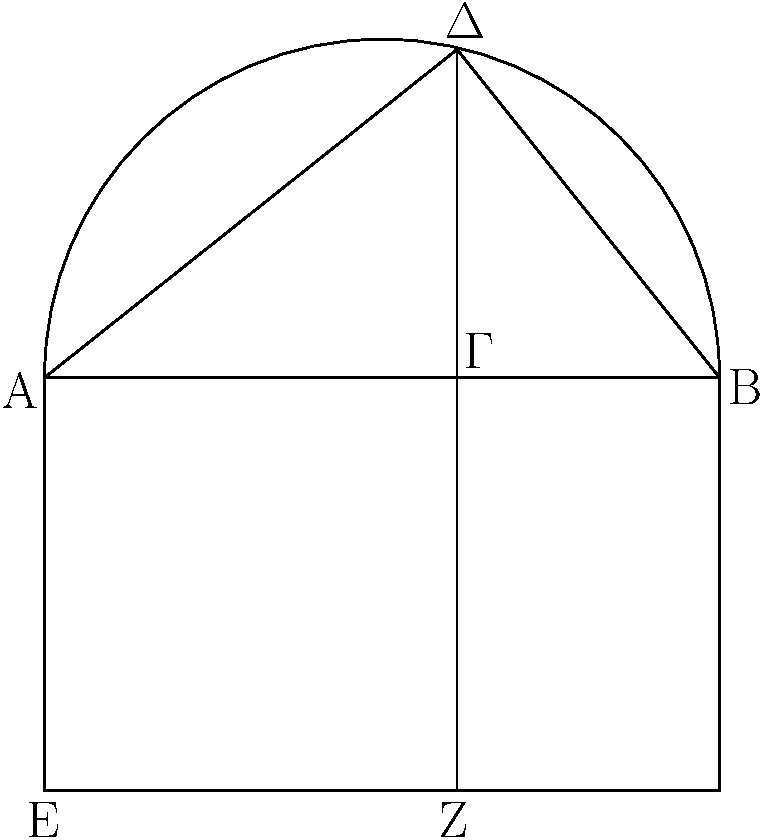
\includegraphics{Book13/fig13ag.pdf}}

\begin{center}\vspace*{-7pt}
{\large \gr{Λῆμμα}.}
\end{center}\vspace*{-7pt}

\gr{Δεικτέον, <ότι ἐστὶν ὡξ ἡ ΑΒ πρὸξ τὴν ΒΓ, ο<ύτωξ
τὸ ἀπὸ τῆξ ΑΔ πρὸξ τὸ ἀπὸ τῆξ ΔΓ.}

\gr{Ἐκκείσθω γὰρ ἡ τοῦ ἡμικυκλίου καταγραφή, καὶ ἐπεζεύθθω
ἡ ΔΒ, καὶ ἀναγεγράφθω ἀπὸ τῆξ ΑΓ τετράγωνον τὸ ΕΓ,
καὶ συμπεπληρώσθω τὸ ΖΒ παραλληλόγραμμον. ἐπεὶ ο>ῦν
διὰ τὸ ἰσογώνιον ε>ῖναι τὸ ΔΑΒ τρίγωνον τῶ| ΔΑΓ
τριγώνῳ ἐστὶν ὡξ ἡ ΒΑ πρὸξ τὴν ΑΔ, ο<ύτωξ ἡ ΔΑ πρὸξ
τὴν ΑΓ, τὸ >άρα ὑπὸ τῶν ΒΑ, ΑΓ >ίσον ἐστὶ τῶ| ἀπὸ
τῆξ ΑΔ. καὶ ἐπεί ἐστιν ὡξ ἡ ΑΒ πρὸξ τὴν ΒΓ, ο<ύτωξ
τὸ ΕΒ πρὸξ τὸ ΒΖ, καί ἐστι τὸ μὲν ΕΒ τὸ ὑπὸ τῶν ΒΑ,
ΑΓ; >ίση γὰρ ἡ ΕΑ τῆ| ΑΓ; τὸ δὲ ΒΖ τὸ ὑπὸ τῶν
ΑΓ, ΓΒ, ὡξ >άρα ἡ ΑΒ πρὸξ τὴν ΒΓ, ο<ύτωξ τὸ ὑπὸ τῶν
ΒΑ, ΑΓ πρὸν
τὸ ὑπὸ τῶν ΑΓ, ΓΒ. καί
ἐστι τὸ μὲν  ὑπὸ τῶν ΒΑ, ΑΓ >ίσον τῶ| ἀπὸ τῆξ ΑΔ, τὸ
δὲ ὑπὸ τῶν ΑΓΒ >ίσον τῶ| ἀπὸ τῆξ ΔΓ; ἡ γὰρ ΔΓ
κάθετοξ τῶν τῆξ βάσεωξ τμ\kern -.7pt  ημάτων τῶν ΑΓ, ΓΒ μέση
ἀνάλογόν ἐστι διὰ τὸ ὀρθὴν ε>ῖναι τὴν ὑπὸ ΑΔΒ.
ὡξ >άρα ἡ ΑΒ πρὸξ τὴν ΒΓ, ο<ύτωξ τὸ ἀπὸ τῆξ
ΑΔ πρὸξ τὸ ἀπὸ τῆξ ΔΓ; <όπερ >έδει δεῖχαι.}}

\ParallelRText{
% Removed epsf size command
\centerline{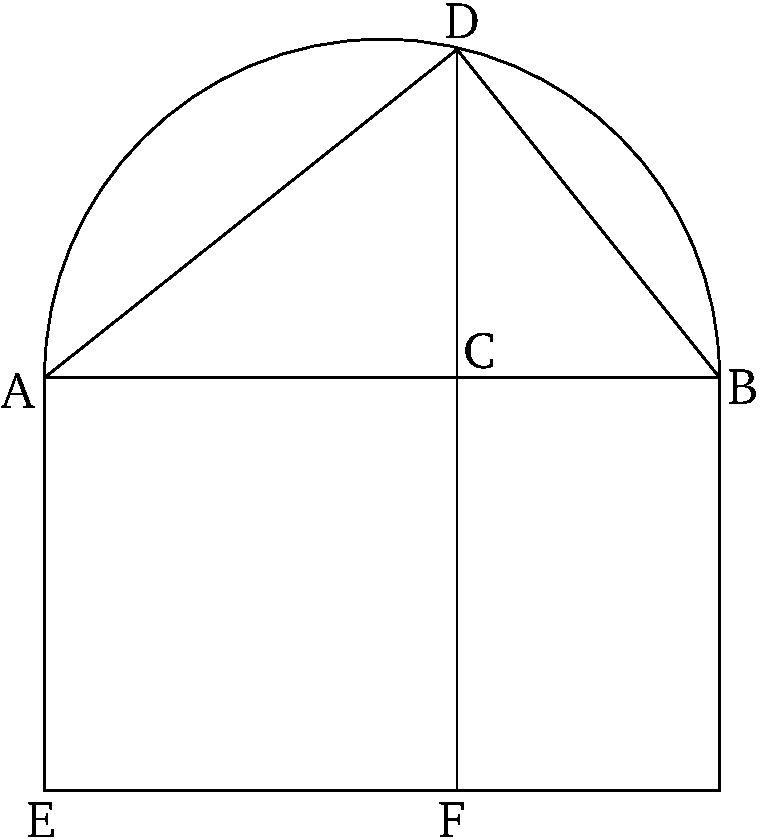
\includegraphics{Book13/fig13ae.pdf}}

\begin{center}
{\large Lemma}
\end{center}

It must be shown that as $AB$ is to $BC$, so the (square) on
$AD$ (is) to the (square) on $DC$.

For, let the figure of the semi-circle be set out, and let $DB$ have
been joined. And let the square $EC$ be described on
$AC$. And let the parallelogram $FB$ be completed. 
Therefore, since, on account of triangle $DAB$ being
equiangular to  triangle $DAC$ [Props.~6.8, 6.4], (proportionally) as $BA$
is to $AD$, so $DA$ (is) to $AC$,  the (rectangle contained)
by $BA$ and $AC$  is thus equal to the (square) on $AD$ [Prop.~6.17]. 
And since as $AB$ is to $BC$, so $EB$ (is) to $BF$ [Prop.~6.1].
And $EB$ is  the (rectangle contained) by $BA$ and $AC$---for $EA$ (is) equal to $AC$. And $BF$  the (rectangle
contained) by $AC$ and $CB$. Thus, as $AB$ (is) to $BC$,
so the (rectangle contained) by $BA$ and $AC$ (is) to the
(rectangle contained) by $AC$ and $CB$. And the (rectangle contained)
by $BA$ and $AC$ is equal to the (square) on $AD$, and the
(rectangle contained) by $ACB$ (is) equal to the (square) on 
$DC$. For the perpendicular $DC$ is the mean proportional
to the pieces  of the base, $AC$ and $CB$, on account of
$ADB$ being a right-angle [Prop.~6.8~corr.]. Thus, as
$AB$ (is) to $BC$, so the (square) on $AD$ (is) to the (square)
on $DC$. (Which is) the very thing it was required to show.}
\end{Parallel}

%%%%
%13.14
%%%%
\pdfbookmark[1]{Proposition 13.14}{pdf13.14}
\begin{Parallel}{}{}
\ParallelLText{
\begin{center}
{\large \ggn{14}.}
\end{center}\vspace*{-7pt}

\gr{Ὀκτάεδρον συστήσασθαι καὶ σφαίρᾳ περιλαβεῖν, <ῆ| καὶ τὰ
πρότερα, καὶ δεῖχαι, <ότι ἡ τῆξ σφαίραξ διάμετροξ δυνάμει
διπλασία ἐστὶ τῆξ πλευρᾶξ τοῦ ὀκταέδρου.}\\

% Removed epsf size command
\centerline{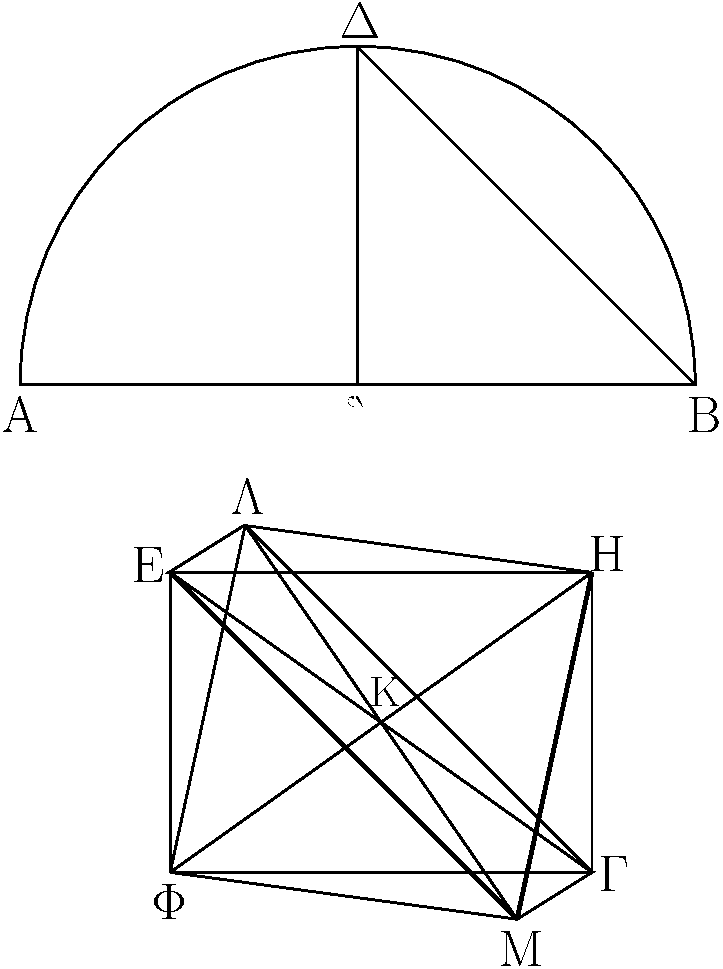
\includegraphics{Book13/fig14g.pdf}}

\gr{Ἐκκείσθω ἡ τῆξ δοθείσηξ σφαίραξ διάμετροξ ἡ ΑΒ, καὶ
τετμ\kern -.7pt  ήσθω δίθα κατὰ τὸ Γ, καὶ γεγράφθω ἐπὶ τῆξ ΑΒ
ἡμικύκλιον τὸ ΑΔΒ, καὶ >ήθθω ἀπὸ τοῦ
Γ τῆ| ΑΒ πρὸξ ὀρθὰξ ἡ ΓΔ,  καὶ ἐπεζεύθθω ἡ ΔΒ,
καὶ ἐκκείσθω τετράγωνον τὸ ΕΖΗΘ >ίσην >έθον ἑκάστην
τῶν πλευρῶν τῆ| ΔΒ, καὶ ἐπεζεύθθωσαν αἱ ΘΖ, ΕΗ, καὶ
ἀνεστάτω ἀπὸ τοῦ Κ σημείου τῶ| τοῦ ΕΖΗΘ τετραγώνου
ἐπιπέδῳ πρὸξ ὀρθὰξ εὐθεῖα ἡ ΚΛ καὶ διήθθω
ἐπὶ τὰ <έτερα μέρη τοῦ ἐπιπέδου ὡξ ἡ ΚΜ, καὶ
ἀφῃρήσθω ἀφ> ἑκατέραξ τῶν ΚΛ, ΚΜ μιᾶ| τῶν ΕΚ, ΖΚ, ΗΚ, ΘΚ
>ίση ἑκατέρα τῶν ΚΛ, ΚΜ, καὶ ἐπεζεύθθωσαν αἱ ΛΕ, ΛΖ, ΛΗ, ΛΘ,
ΜΕ, ΜΖ, ΜΗ, ΜΘ.}

\gr{Καὶ ἐπεὶ >ίση ἐστὶν ἡ ΚΕ τῆ| ΚΘ, καί
ἐστιν ὀρθὴ ἡ ὑπὸ ΕΚΘ γωνία, τὸ >άρα ἀπὸ τῆξ ΘΕ
διπλάσιόν ἐστι τοῦ ἀπὸ τῆξ ΕΚ. πάλιν, ἐπεὶ >ίση ἐστὶν
ἡ ΛΚ τῆ| ΚΕ, καί ἐστιν ὀρθὴ ἡ ὑπὸ ΛΚΕ γωνία,
τὸ >άρα ἀπὸ τῆξ ΕΛ διπλάσιόν ἐστι τοῦ ἀπὸ ΕΚ.
ἐδείθθη δὲ καὶ τὸ ἀπὸ τῆξ ΘΕ διπλάσιον τοῦ ἀπὸ τῆξ
ΕΚ; τὸ >άρα ἀπὸ τῆξ ΛΕ >ίσον ἐστὶ τῶ| ἀπὸ τῆξ
ΕΘ; >ίση >άρα ἐστὶν ἡ ΛΕ τῆ| ΕΘ. διὰ τὰ α\kern -.7pt  ὐτὰ δὴ καὶ ἡ
ΛΘ τῆ| ΘΕ ἐστιν >ίση; ἰσόπλευρον >άρα ἐστὶ τὸ ΛΕΘ τρίγωνον.
ὁμοίωξ δὴ δείχομεν, <ότι καὶ <έκαστον τῶν λοιπῶν
τριγώνων, <ῶν βάσειξ μέν εἰσιν αἱ τοῦ ΕΖΗΘ τετραγώνου
πλευραί, κορυφαὶ δὲ τὰ Λ, Μ σημεῖα, ἰσόπλευρόν ἐστιν; ὀκτάεδρον
>άρα συνέσταται ὑπὸ ὀκτὼ τριγώνων ἰσοπλεύρων περιεχόμενον.}

\gr{Δεῖ δὴ α\kern -.7pt  ὐτὸ καὶ σφαίρᾳ περιλαβεῖν τῆ| δοθείσῃ καὶ
δεῖχαι, <ότι ἡ τῆξ σφαίραξ διάμετροξ δυνάμει διπλασίων
ἐστὶ τῆξ τοῦ ὀκταέδρου πλευρᾶξ.}

\gr{Ἐπεὶ γὰρ αἱ τρεῖξ αἱ ΛΚ, ΚΜ, ΚΕ >ίσαι
ἀλλήλαιξ εἰσίν, τὸ >άρα ἐπὶ τῆξ ΛΜ γραφόμενον
ἡμικύκλιον <ήχει καὶ διὰ τοῦ Ε. καὶ διὰ τὰ α\kern -.7pt  ὐτά,
ἒαν μενούσηξ τῆξ ΛΜ περιενεθθὲν τὸ ἡμικύκλιον
εἰξ τὸ α\kern -.7pt  ὐτὸ ἀποκατασταθῆ|, <όθεν >ήρχατο φέρεσθαι,
<ήχει καὶ διὰ τῶν Ζ, Η, Θ σημείων, καὶ >έσται σφαίρᾳ
περιειλημμένον τὸ ὀκτάεδρον. λέγω δή, <ότι καὶ τῆ| δοθείσῃ.
ἐπεὶ γὰρ >ίση ἐστὶν ἡ ΛΚ τῆ| ΚΜ, κοινὴ δὲ ἡ ΚΕ, καὶ
γωνίαξ ὀρθὰξ περιέθουσιν, βάσιξ >άρα ἡ ΛΕ βάσει τῆ| ΕΜ
ἐστιν >ίση. καὶ ἐπεὶ ὀρθή ἐστιν ἡ ὑπὸ ΛΕΜ γωνία;
ἐν ἡμικυκλίῳ γάρ; τὸ >άρα ἀπὸ τῆξ ΛΜ διπλάσιόν
ἐστι τοῦ ἀπὸ τῆξ ΛΕ. πάλιν, ἐπεὶ >ίση ἐστὶν ἡ ΑΓ τῆ|
ΓΒ, διπλασία ἐστὶν ἡ ΑΒ τῆξ ΒΓ. ὡξ δὲ ἡ ΑΒ πρὸξ τὴν
ΒΓ, ο<ύτωξ τὸ ἀπὸ τῆξ ΑΒ πρὸξ τὸ ἀπὸ τῆξ ΒΔ; διπλάσιον
>άρα ἐστὶ τὸ ἀπὸ τῆξ ΑΒ τοῦ ἀπὸ τῆξ ΒΔ. ἐδείθθη
δὲ καὶ τὸ ἀπὸ τῆξ ΛΜ διπλάσιον τοῦ ἀπὸ τῆξ ΛΕ.
καί ἐστιν >ίσον τὸ ἀπὸ τῆξ ΔΒ τῶ| ἀπὸ τῆξ ΛΕ;
>ίση γὰρ κεῖται ἡ ΕΘ τῆ| ΔΒ. >ίσον >άρα καὶ τὸ ἀπὸ τῆξ
ΑΒ τῶ| ἀπὸ τῆξ ΛΜ; >ίση >άρα ἡ ΑΒ τῆ| ΛΜ. καί ἐστιν
ἡ ΑΒ ἡ τῆξ δοθείσηξ σφαίραξ διάμετροξ; ἡ ΛΜ >άρα >ίση
ἐστὶ τῆ| τῆξ δοθείσηξ σφαίραξ διαμέτρῳ.}

\gr{Περιείληπται >άρα τὸ ὀκτάεδρον τῆ| δοθείσῃ σφαίρᾳ.
καὶ συναποδέδεικται, <ότι ἡ τῆξ σφαίραξ διάμετροξ δυνάμει
διπλασίων ἐστὶ τῆξ τοῦ ὀκταέδρου πλευρᾶξ; <όπερ
>έδει δεῖχαι.}}

\ParallelRText{
\begin{center}
{\large Proposition 14}
\end{center}

To construct an octahedron, and to enclose (it) in a (given) sphere, like in the preceding (proposition), and to show that the square
on the diameter of the sphere is double the (square) on the
side of the octahedron.

% Removed epsf size command
\centerline{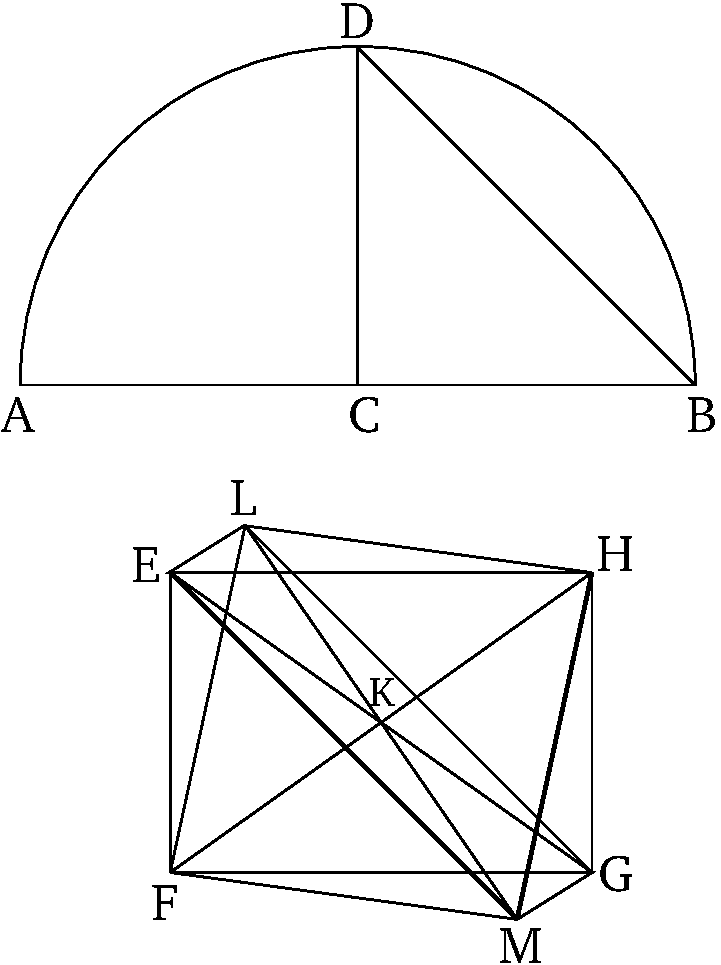
\includegraphics{Book13/fig14e.pdf}}

Let the diameter $AB$ of the given sphere be laid out, and let it have
been cut in half at $C$. And let the semi-circle $ADB$ be
drawn on $AB$. And let $CD$ be drawn from $C$ at right-angles to
$AB$. And let $DB$ be joined. And let the square $EFGH$,
having each of its sides equal to $DB$, be laid out. And let $HF$
and $EG$ be joined. And let the straight-line $KL$
be set up, at point $K$, at right-angles to the plane of square 
$EFGH$ [Prop.~11.12]. And let it be drawn across  on the other side of
the plane, like $KM$. And let $KL$ and $KM$, equal to
one of $EK$, $FK$, $GK$, and $HK$,  be cut off from 
$KL$ and $KM$, respectively. And let $LE$, $LF$, $LG$, $LH$, $ME$, $MF$,
$MG$, and $MH$ be joined.  

And since  $KE$ is equal to $KH$, and angle $EKH$ is a right-angle, 
the (square) on the  $HE$ is thus double the (square) on $EK$ [Prop.~1.47].
Again, since $LK$ is equal to $KE$, and angle $LKE$
is a right-angle, the (square) on $EL$ is thus double the (square) on
$EK$ [Prop.~1.47]. And the (square) on $HE$ was also shown (to be)
double the (square) on $EK$.  Thus, the (square) on $LE$
is equal to the (square) on $EH$. Thus, $LE$ is equal to $EH$. So,
for the same (reasons), $LH$ is also equal to $HE$. Triangle
$LEH$ is thus equilateral. So, similarly, we can show that each of
the remaining triangles, whose bases are the sides of the
square $EFGH$, and apexes the points $L$ and $M$, are equilateral.
Thus, an octahedron contained by eight
equilateral triangles has been constructed.

So, it is also necessary to enclose it by the given sphere, and to show that the
square on the diameter of the sphere is double the (square) on the
side of the octahedron.

For since the three (straight-lines) $LK$, $KM$, and $KE$ are equal
to one another, the semi-circle drawn on $LM$ will thus also pass
through $E$. And, for the same (reasons), if $LM$ remains (fixed), and the semi-circle is carried around, and again established at the same
(position) from which it began to be moved, then it will also pass
through points $F$, $G$, and $H$, and the octahedron will be
enclosed by a sphere. So, I say that (it is) also (enclosed)
by the given (sphere). For since $LK$ is equal to $KM$, and $KE$
(is) common, and they contain right-angles, the base
$LE$ is thus equal to the base $EM$ [Prop.~1.4]. And since angle $LEM$
is a right-angle---for (it is) in a semi-circle [Prop.~3.31]---the
(square) on $LM$ is thus double the (square) on $LE$ [Prop.~1.47]. 
Again, since $AC$ is equal to $CB$, $AB$ is double $BC$. 
And as $AB$ (is) to $BC$, so the (square) on $AB$ (is) to the
(square) on $BD$ [Prop.~6.8, Def.~5.9]. Thus, the (square) on 
$AB$ is double the (square) on $BD$. And the (square) on $LM$
was also shown (to be) double the (square) on $LE$. And the (square)
on $DB$ is equal to the (square) on $LE$. For $EH$ was made equal
to $DB$. Thus, the (square) on $AB$ (is) also equal to the (square) on 
$LM$. Thus, $AB$ (is) equal to $LM$. And $AB$ is the diameter of the
given sphere. Thus, $LM$ is equal to the diameter of the given sphere.

Thus, the octahedron has been enclosed by the given sphere,  and it has
been simultaneously  proved that the square on the diameter of the sphere
is double the (square) on the side of the octahedron.$^\dag$ (Which is) the
very thing it was required to show.}
\end{Parallel}
{\footnotesize\noindent$^\dag$ If the radius of the sphere is unity then the
side of octahedron is $\sqrt{2}$.}

%%%%
%13.15
%%%%
\pdfbookmark[1]{Proposition 13.15}{pdf13.15}
\begin{Parallel}{}{}
\ParallelLText{
\begin{center}
{\large \ggn{15}.}
\end{center}\vspace*{-7pt}

\gr{Κύβον συστήσασθαι καὶ σφαίρᾳ περιλαβεῖν, <ῆ| καὶ τὴν
πυραμίδα, καὶ δεῖχαι, <ότι ἡ τῆξ σφαίραξ διάμετροξ δυνάμει
τριπλασίων ἐστὶ τῆξ τοῦ κύβου πλευρᾶξ.}

\gr{Ἐκκείσθω ἡ τῆξ δοθείσηξ σφαίραξ διάμετροξ ἡ ΑΒ καὶ
τετμ\kern -.7pt  ήσθω κατὰ τὸ Γ <ώστε διπλῆν ε>ῖναι τὴν ΑΓ τῆξ
ΓΒ, καὶ γεγράφθω ἐπὶ τῆξ ΑΒ ἡμικύκλιον τὸ ΑΔΒ, καὶ
ἀπὸ τοῦ Γ τῆ| ΑΒ πρὸξ ὀρθὰξ >ήθθω ἡ ΓΔ, καὶ
ἐπεζεύθθω ἡ ΔΒ, καὶ ἐκκείσθω τετράγωνον τὸ ΕΖΗΘ
>ίσην >έθον τὴν πλευρὰν τῆ| ΔΒ, καὶ ἀπὸ τῶν Ε, Ζ, Η, Θ
τῶ| τοῦ ΕΖΗΘ τετραγώνου ἐπιπέδῳ πρὸξ ὀρθὰξ >ήθθωσαν
αἱ ΕΚ, ΖΛ, ΗΜ, ΘΝ, καὶ ἀφῃρήσθω ἀπὸ ἑκάστηξ
τῶν ΕΚ, ΖΛ, ΗΜ, ΘΝ μιᾶ| τῶν ΕΖ, ΖΗ, ΗΘ, ΘΕ >ίση
ἑκάστη τῶν ΕΚ, ΖΛ, ΗΜ, ΘΝ, καὶ ἐπεζεύθθωσαν αἱ ΚΛ,
ΛΜ, ΜΝ, ΝΚ; κύβοξ >άρα συνέσταται ὁ ΖΝ ὑπὸ <ὲχ
τετραγώνων >ίσων περιεθόμενοξ.}

\gr{Δεῖ δὴ α\kern -.7pt  ὐτὸν καὶ σφαίρᾳ
περιλαβεῖν τῆ| δοθείσῃ καὶ δεῖχαι, <ότι ἡ τῆξ σφαίραξ
διάμετροξ δυνάμει τριπλασία ἐστὶ τῆξ πλευρᾶξ τοῦ κύβου.}\\

% Removed epsf size command
\centerline{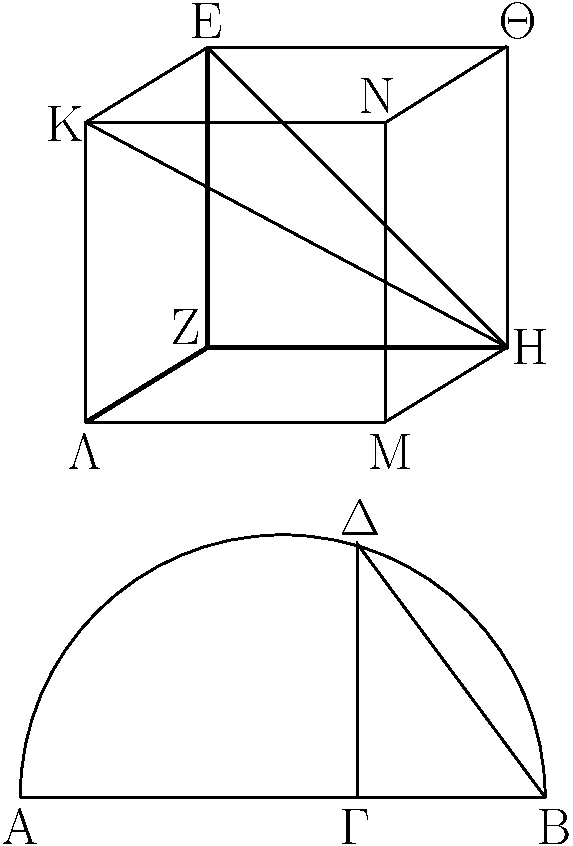
\includegraphics{Book13/fig15g.pdf}}

\gr{Ἐπεζεύθθωσαν γὰρ αἱ ΚΗ, ΕΗ. καὶ ἐπεὶ ὀρθή
ἐστιν ἡ ὑπὸ ΚΕΗ γωνία διὰ τὸ καὶ τὴν ΚΕ ὀρθὴν
ε>ῖναι πρὸξ τὸ ΕΗ ἐπίπεδον δηλαδὴ καὶ πρὸξ τὴν ΕΗ
εὐθεῖαν, τὸ >άρα ἐπὶ τῆξ ΚΗ γραφόμενον ἡμικύκλιον
<ήχει καὶ διὰ τοῦ Ε σημείου. πάλιν, ἐπεὶ ἡ ΗΖ ὀρθή
ἐστι πρὸξ ἑκατέραν τῶν ΖΛ, ΖΕ, καὶ πρὸξ τὸ ΖΚ >άρα
ἐπίπεδον ὀρθή ἐστιν ἡ ΗΖ; <ώστε καὶ ἒαν ἐπιζεύχωμεν
τὴν ΖΚ, ἡ ΗΖ ὀρθὴ >έσται καὶ πρὸξ τὴν ΖΚ;
καὶ δὶα τοῦτο πάλιν τὸ ἐπὶ τῆξ ΗΚ γραφόμενον ἡμικύκλιον
<ήχει καὶ διὰ τοῦ Ζ. ὁμοίωξ καὶ δὶα τῶν λοιπῶν
τοῦ κύβου σημείων <ήχει. ἒαν δὴ μενούσηξ τῆξ ΚΗ
περιενεθθὲν τὸ ἡμικύκλιον εἰξ τὸ α\kern -.7pt  ὐτὸ ἀποκατασταθῆ|, 
<όθεν >ήρχατο φέρεσθαι, >έσται σφαίρᾳ περιειλημμένοξ
ὁ κύβοξ. λέγω δή, <ότι καὶ τῆ| δοθείσῃ. ἐπεὶ γὰρ >ίση ἐστὶν
ἡ ΗΖ τῆ| ΖΕ, καί ἐστιν ὀρθὴ ἡ πρὸξ τῶ| Ζ γωνία, τὸ >άρα
ἀπὸ τῆξ ΕΗ διπλάσιόν ἐστι τοῦ ἀπὸ τῆξ ΕΖ. >ίση δὲ ἡ ΕΖ
τῆ| ΕΚ; τὸ  >άρα ἀπὸ τῆξ ΕΗ διπλάσιόν ἐστι τοῦ ἀπὸ
τῆξ ΕΚ; <ώστε τὰ ἀπὸ τῶν ΗΕ, ΕΚ, τουτέστι τὸ ἀπὸ τῆξ
ΗΚ, τριπλάσιόν ἐστι τοῦ ἀπὸ τῆξ ΕΚ. καὶ ἐπεὶ τριπλασίων
ἐστὶν ἡ ΑΒ τῆξ ΒΓ, ὡξ δὲ ἡ ΑΒ πρὸξ τὴν ΒΓ, ο<ύτωξ
τὸ ἀπὸ τῆξ ΑΒ πρὸξ τὸ ἀπὸ τῆξ ΒΔ, τριπλάσιον >άρα τὸ
ἀπὸ τῆξ ΑΒ τοῦ ἀπὸ τῆξ ΒΔ. ἐδείθθη δὲ καὶ τὸ ἀπὸ
τῆξ ΗΚ τοῦ ἀπὸ τῆξ ΚΕ τριπλάσιον. καὶ κεῖται >ίση
ἡ ΚΕ τῆ| ΔΒ; >ίση >άρα καὶ ἡ ΚΗ τῆ| ΑΒ. καί
ἐστιν ἡ ΑΒ τῆξ δοθείσηξ σφαίραξ διάμετροξ; καὶ ἡ ΚΗ
>άρα >ίση ἐστὶ τῆ| τῆξ δοθείσηξ σφαίραξ διαμέτρῳ.}

\gr{Τῆ| δοθείσῃ >άρα σφαίρα περιείληπται ὁ κύβοξ; καὶ συναποδέδεικται,
<ότι ἡ τῆξ σφαίραξ διάμετροξ δυνάμει τριπλασίων ἐστὶ
τῆξ τοῦ κύβου πλευρᾶξ; <όπερ >έδει δεῖχαι.}}

\ParallelRText{
\begin{center}
{\large Proposition 15}
\end{center}

To construct a cube, and to enclose (it) in a sphere, like in the (case of the)
pyramid, and to show that the square on the diameter of the sphere
is three times the (square) on the side of the cube.

Let the diameter $AB$ of the given sphere be laid out, and let it be
cut at $C$ such that $AC$ is double $CB$. And let the semi-circle
$ADB$ be drawn on $AB$. And let $CD$ be drawn from $C$
at right-angles to $AB$. And let $DB$ be joined. And let the
square $EFGH$, having (its) side equal to $DB$, be laid out. And
let $EK$, $FL$, $GM$, and $HN$ be drawn from (points)
$E$, $F$, $G$, and $H$, (respectively), at right-angles to the plane of
square $EFGH$. And let $EK$, $FL$, $GM$, and $HN$, equal
to one of $EF$, $FG$, $GH$, and $HE$, be cut off from
$EK$, $FL$, $GM$, and $HN$, respectively. And let $KL$,
$LM$, $MN$, and $NK$ be joined. Thus, a cube contained
by six equal squares has been constructed. 

So, it is also necessary
to enclose it by the given sphere, and to show that the square on
the diameter of the sphere is three times the (square) on the side of the cube.

% Removed epsf size command
\centerline{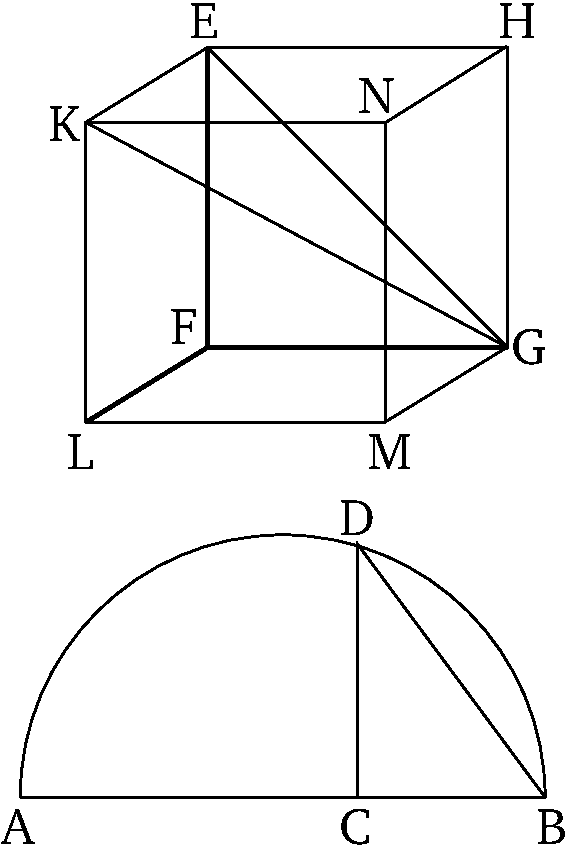
\includegraphics{Book13/fig15e.pdf}}

For let $KG$ and $EG$ be joined. And since
angle $KEG$ is a right-angle---on account of $KE$ also being at right-angles
to the plane $EG$, and manifestly also to the straight-line $EG$ [Def.~11.3]---the semi-circle drawn on $KG$ will thus also pass through
point $E$. Again, since $GF$ is at right-angles to each of $FL$
and $FE$, $GF$ is thus also at right-angles to the plane $FK$ [Prop.~11.4]. 
Hence, if we also join $FK$ then $GF$ will also be at right-angles to
$FK$. And, again, on account of this, the semi-circle drawn on
$GK$ will also pass through point $F$. Similarly, it will also pass through
the remaining (angular) points of the cube. So, if $KG$ remains (fixed), 
and the semi-circle is carried around, and again established at the
same (position) from which it began to be moved, then the cube will
be enclosed by a sphere. So, I say that (it is) also (enclosed)
by the given (sphere). For since $GF$ is equal to $FE$, and the
angle at $F$ is a right-angle, the (square) on $EG$ is thus double
the (square) on $EF$ [Prop.~1.47]. And $EF$ (is) equal to
$EK$. Thus, the (square) on $EG$ is double the (square) on $EK$.
Hence, the (sum of the squares) on $GE$ and $EK$---that is to say, the
(square) on $GK$ [Prop.~1.47]---is three times the  (square) on $EK$. And since
$AB$ is three times $BC$, and as $AB$ (is) to $BC$, so the
(square) on $AB$ (is) to the (square) on $BD$ [Prop.~6.8, Def.~5.9], 
the (square) on $AB$ (is) thus three times the (square) on $BD$. 
And the (square) on $GK$ was also shown (to be) three times
the (square) on $KE$. And $KE$ was made equal to $DB$. 
Thus, $KG$ (is) also equal to $AB$. And $AB$ is the
radius of the given sphere. Thus, $KG$ is also equal to the diameter of the
given sphere.

Thus, the cube has been enclosed by the given sphere. And it
has simultaneously been shown that the square on the diameter of
the sphere is three times the (square) on the side of the cube.$^\dag$ (Which is)
the very thing it was required to show.}
\end{Parallel}
{\footnotesize\noindent$^\dag$ If the radius of the sphere is unity 
then the side of the cube is $\sqrt{4/3}$.}

%%%%
%13.16
%%%%
\pdfbookmark[1]{Proposition 13.16}{pdf13.16}
\begin{Parallel}{}{}
\ParallelLText{
\begin{center}
{\large \ggn{16}.}
\end{center}\vspace*{-7pt}

\gr{Εἰκοσάεδρον συστήσασθαι καὶ σφαίρᾳ περιλαβεῖν,
<ῆ| καὶ τὰ προειρημένα σθήματα, καὶ δεῖχαι, <ότι
ἡ τοῦ εἰκοσαέδρου πλευρὰ >άλογόξ ἐστιν ἡ καλουμένη
ἐλάττων.}

% Removed epsf size command
\centerline{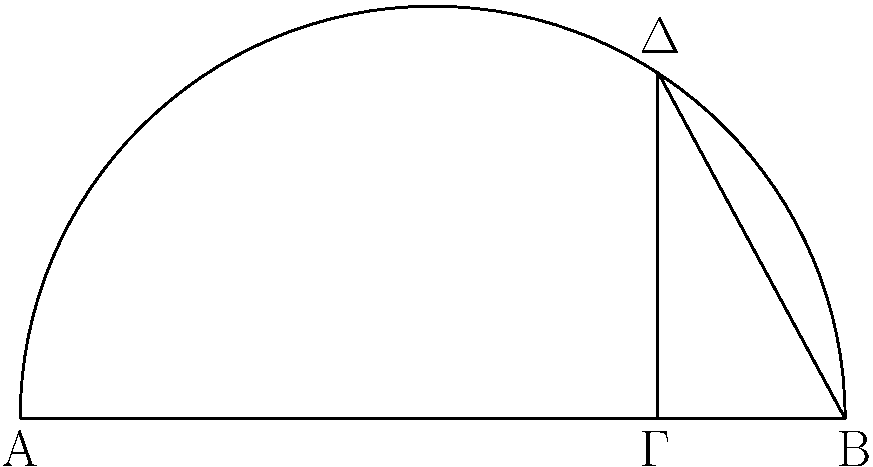
\includegraphics{Book13/fig16ag.pdf}}

\gr{Ἐκκείσθω ἡ τῆξ δοθείσηξ σφαίραξ διάμετροξ
ἡ ΑΒ καὶ τετμ\kern -.7pt  ήσθω κατὰ τὸ Γ <ώστε τετραπλῆν ε>ῖναι
τὴν ΑΓ τῆξ ΓΒ, καὶ γεγράφθω ἐπὶ τῆξ ΑΒ ἡμικύκλιον
τὸ ΑΔΒ, καὶ >ήθθω ἀπὸ τοῦ Γ τῆ| ΑΒ πρὸξ ορθὰξ
γωνίαξ εὐθεῖα γραμμ\kern -.7pt  ὴ ἡ ΓΔ, καί ἐπεζεύθθω ἡ ΔΒ,
καὶ ἐκκείσθω κύκλοξ ὁ ΕΖΗΘΚ, ο<ῦ ἡ ἐν τοῦ κέντρου
>ίση >έστω τῆ| ΔΒ, καὶ ἐγγεγράφθω εἰξ τὸν
ΕΖΗΘΚ κύκλον πεντάγωνον ἰσόπλευρόν τε καὶ ἰσογώνιον
τὸ ΕΖΗΘΚ, καὶ τετμ\kern -.5pt  ήσθωσαν αἱ ΕΖ, ΖΗ, ΗΘ, ΘΚ, ΚΕ περιφέρειαι
δίθα κατὰ τὸ Λ, Μ, Ν, Χ, Ο σημεῖα, καὶ ἐπεζεύθθωσαν αἱ
ΛΜ, ΜΝ, ΝΧ, ΧΟ, ΟΛ, ΕΟ. >ίσόπλευρον >άρα ἐστὶ καὶ τὸ
ΛΜΝΧΟ πεντάγωνον, καὶ δεκαγώνου ἡ ΕΟ εὐθεῖα.
καὶ ἀνεστάτωσαν >άπὸ τῶν Ε, Ζ, Η, Θ, Κ σημείων
τῶ| τοῦ κύκλου ἐπιπέδῳ πρὸξ ὀρθὰξ γωνίαξ
εὐθεῖαι αἱ ΕΠ, ΖΡ, ΗΣ, ΘΤ, ΚΥ >ίσαι ο>ῦσαι τῆ| ἐκ
τοῦ κέντρου τοῦ ΕΖΗΘΚ κύκλου, καὶ ἐπεζεύθθωσαν
αἱ ΠΡ, ΡΣ, ΣΤ, ΤΥ, ΥΠ, ΠΛ, ΛΡ, ΡΜ, ΜΣ, ΣΝ, ΝΤ, ΤΧ, ΧΥ,
ΥΟ, ΟΠ.}

\gr{Καὶ ἐπεὶ ἑκατέρα τῶν ΕΠ, ΚΥ τῶ| α\kern -.7pt  ὐτῶ| ἐπιπέδῳ
πρὸξ ὀρθάξ ἐστιν, παράλληλοξ >άρα ἐστὶν ἡ ΕΠ
τῆ| ΚΥ. >έστι δὲ α\kern -.7pt  ὐτῆ| καὶ >ίση; αἱ δὲ τὰξ >ίσαξ
τε καὶ παραλλήλουξ ἐπιζευγνύουσαι ἐπὶ τὰ α\kern -.5pt  ὐτὰ μέρη
εὐθεῖαι >ίσαι τε καὶ παράλληλοί εἰσιν. ἡ ΠΥ >άρα τῆ|
ΕΚ >ίση τε καὶ παράλληλόξ ἐστιν. πενταγώνου δὲ
ἰσοπλεύρου ἡ ΕΚ; πενταγώνου >άρα ἰσοπλεύρου
καὶ ἡ ΠΥ τοῦ εἰξ τὸν ΕΖΗΘΚ κύκλον ἐγγραφομένου.
διὰ τὰ α\kern -.3pt  ὐτὰ δὴ καὶ ἑκάστη τῶν ΠΡ, ΡΣ, ΣΤ, ΤΥ πενταγώνου
ἐστὶν ἰσοπλεύρου τοῦ εἰξ τὸν ΕΖΗΘΚ κύκλον ἐγγραφομένου;
ἰσόπλευρον >άρα τὸ ΠΡΣΤΥ πεντάγωνον. καὶ ἐπεὶ ἑχαγώνου
μέν ἐστιν ἡ ΠΕ, δεκαγώνου δὲ ἡ ΕΟ, καί ἐστιν ὀρθὴ ἡ ὑπὸ
ΠΕΟ, πενταγώνου >άρα ἐστὶν ἡ ΠΟ; ἡ γὰρ τοῦ πενταγώνου
πλευρὰ δύναται τήν τε τοῦ ἑχαγώνου καὶ τὴν τοῦ
δεκαγώνου τῶν εἰξ τὸν α\kern -.7pt  ὐτὸν κύκλον ἐγγραφομένων.
διὰ τὰ α\kern -.7pt  ὐτὰ δὴ καὶ ἡ ΟΥ πενταγώνου ἐστὶ πλευρά.
>έστι δὲ καὶ ἡ ΠΥ πενταγώνου; ἰσόπλευρον >άρα ἐστὶ
τὸ ΠΟΥ τρίγωνον. διὰ τὰ α\kern -.7pt  ὐτὰ δὴ καὶ <έκαστον τῶν ΠΛΡ, ΡΜΣ, ΣΝΤ,
ΤΧΥ ἰσόπλευρόν ἐστιν. καὶ ἐπεὶ πενταγώνου ἐδείθθη ἑκατέρα
τῶν ΠΛ, ΠΟ, >έστι δὲ καὶ ἡ ΛΟ πενταγώνου, ἰσόπλευρον >άρα
ἐστὶ τὸ ΠΛΟ τρίγωνον. διὰ τὰ α\kern -.7pt  ὐτὰ δὴ καὶ <έκαστον τῶν
ΛΡΜ, ΜΣΝ, ΝΤΧ, ΧΥΟ τριγώνων ἰσόπλευρόν ἐστιν.}~\\~\\~\\~\\

% Removed epsf size command
\centerline{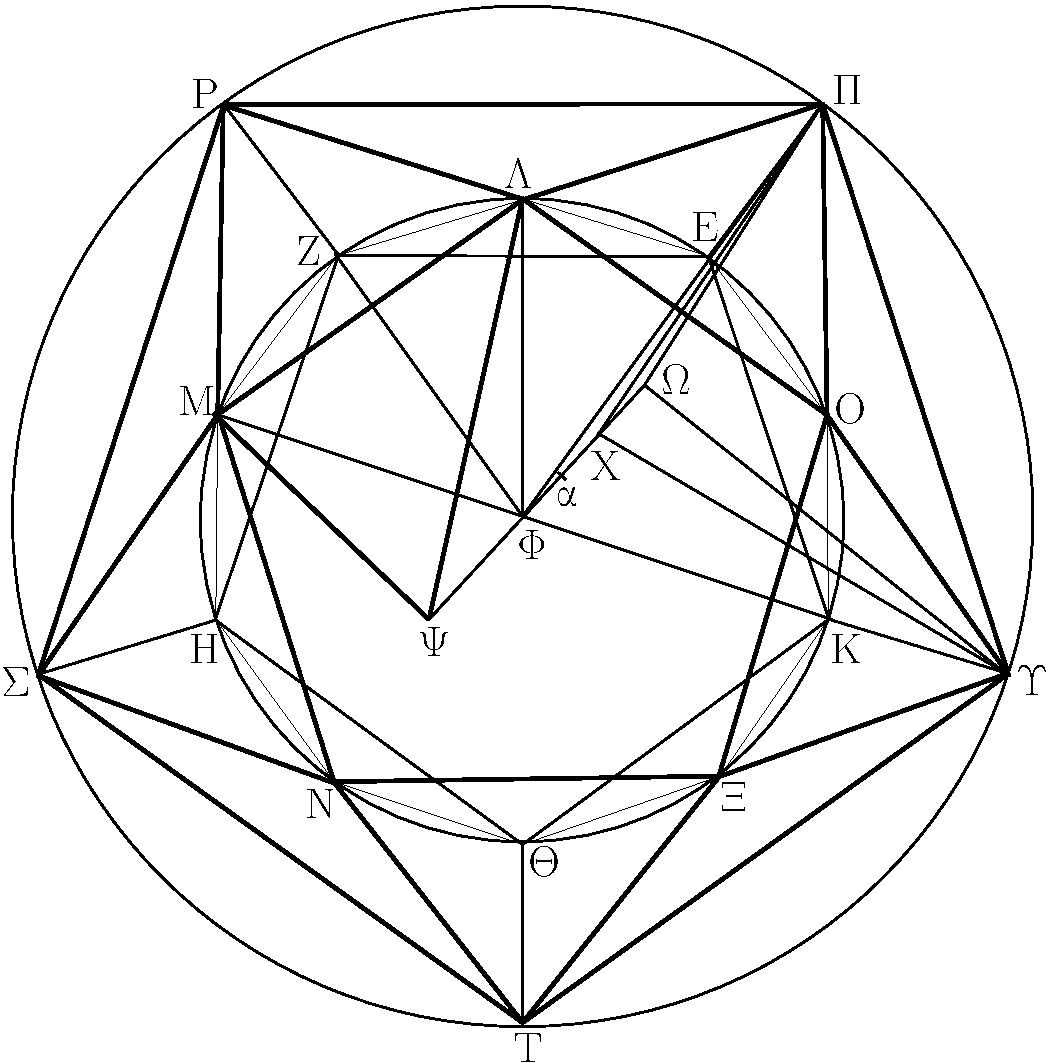
\includegraphics{Book13/fig16g.pdf}}

\gr{Εἰλήφθω
τὸ κέντρον τοῦ ΕΖΗΘΚ κύκλου τὸ Φ σημεῖον; καὶ ἀπὸ
τοῦ Φ τῶ| τοῦ κύκλου ἐπιπέδῳ πρὸξ ὀρθὰξ
ἀνεστάτω ἡ ΦΩ, καὶ ἐκβεβλήσθω ἐπὶ τὰ
<έτερα μέρη ὡξ ἡ ΦΨ, καὶ ἀφῃρήσθω ἑχαγώνου μὲν
ἡ ΦΘ, δεκαγώνου δὲ ἑκατέρα τῶν ΦΨ, ΘΩ, καὶ ἐπεζεύθθωσαν αἱ ΠΩ, ΠΘ, ΥΩ, ΕΦ, ΛΦ, ΛΨ,
ΨΜ.}

\gr{Καὶ ἐπεὶ ἑκατέρα τῶν ΦΘ, ΠΕ τῶ| τοῦ κύκλου
ἐπιπέδῳ πρὸξ ὀρθάξ ἐστιν, παράλληλοξ >άρα ἐστὶν
ἡ ΦΘ τῆ| ΠΕ. εἰσὶ δὲ καὶ >ίσαι; καὶ αἱ ΕΦ, ΠΘ
>άρα >ίσαι τε καὶ παράλληλοί εἰσιν. ἑχαγώνου δὲ ἡ ΕΦ; 
ἑχαγώνου >άρα καὶ ἡ ΠΘ. καὶ ἐπεὶ ἑχαγώνου
μέν ἐστιν ἡ ΠΘ, δεκαγώνου δὲ ἡ ΘΩ, καὶ ὀρθή ἐστιν
ἡ ὑπὸ ΠΘΩ γωνία, πενταγώνου >άρα ἐστὶν ἡ ΠΩ.
διὰ τὰ α\kern -.7pt  ὐτὰ δὴ καὶ ἡ ΥΩ πενταγώνου ἐστίν, ἐπειδήπερ,
ἒαν ἐπιζεύχωμεν τὰξ ΦΚ, ΘΥ, >ίσαι καὶ ἀπεναντίον
>έσονται, καί ἐστιν ἡ ΦΚ ἐκ τοῦ κέντρου ο>ῦσα
ἑχαγώνου.  ἑχαγώνου >άρα καὶ ἡ ΘΥ. δεκαγώνου
δὲ ἡ ΘΩ, καὶ ὀρθὴ ἡ ὑπὸ ΥΘΩ; πενταγώνου
>άρα ἡ ΥΩ. >έστι δὲ καὶ ἡ ΠΥ πενταγώνου; ἰσόπλευρον >άρα
ἐστὶ τὸ ΠΥΩ τρίγωνον. διὰ τὰ α\kern -.7pt  ὐτὰ δὴ καὶ <έκαστον
τῶν λοιπῶν τριγώνων, <ῶν βάσειξ μέν εἰσιν αἱ ΠΡ, ΡΣ,
ΣΤ, ΤΥ εὐθεῖαι, κορυφὴ δὲ τὸ Ω σημεῖον,  ἰσόπλευρόν
ἐστιν. πάλιν, ἐπεὶ ἑχαγώνου μὲν ἡ ΦΛ, δεκαγώνου
δὲ ἡ ΦΨ, καὶ ὀρθή ἐστιν ἡ ὑπὸ ΛΦΨ γωνία, πενταγώνου
>άρα ἐστὶν ἡ ΛΨ. διὰ τὰ α\kern -.5pt  ὐτὰ δὴ ἒαν ἐπιζεύχωμεν τὴν
ΜΦ ο>ῦσαν ἑχαγώνου, συνάγεται καὶ ἡ ΜΨ πενταγώνου.
>έστι δὲ καὶ ἡ ΛΜ πενταγώνου; ἰσόπλευρον >άρα ἐστὶ τὸ
ΛΜΨ τρίγωνον. ὁμοίωξ δὴ δειθθήσεται, <ότι καὶ <έκαστον
τῶν λοιπῶν τριγώνων, <ῶν βάσειξ μέν εἰσιν αἱ ΜΝ,
ΝΧ, ΧΟ, ΟΛ, κορυφὴ δὲ τὸ Ψ σημεὶον, ἰσόπλευρόν
ἐστιν. συνέσταται >άρα εἰκοσάεδρον ὑπὸ ε>ίκοσι τριγώνων
ἰσοπλεύρων περιεχόμενον.}

\gr{Δεῖ δὴ α\kern -.7pt  ὐτὸ καὶ σφαίρᾳ περιλαβεῖν τῆ| δοθείσῃ
καὶ δεῖχαι, <ότι ἡ τοῦ εἰκοσαέδρου πλευρὰ >άλογόξ
ἐστιν ἡ καλουμένη ἐλάσσων.}

\gr{Ἐπεὶ γὰρ ἑχαγώνου ἐστὶν ἡ ΦΘ, δεκαγώνου δὲ ἡ ΘΩ,
ἡ ΦΩ >άρα >άκρον καὶ μέσον λόγον τέτμ\kern -.7pt  ηται κατὰ τὸ Θ,
καὶ τὸ μεῖζον α\kern -.7pt  ὐτῆξ τμ\kern -.5pt  ῆμά ἐστιν ἡ ΦΘ; >έστιν
>άρα ὡξ ἡ ΩΦ πρὸξ τὴν ΦΘ, ο<ύτωξ ἡ ΦΘ πρὸξ
τὴν ΘΩ. >ίση δὲ ἡ μὲν ΦΘ τῆ| ΦΕ, ἡ δὲ ΘΩ
τῆ| ΦΨ; >έστιν >άρα ὡξ ἡ ΩΦ πρὸξ τὴν ΦΕ, ο<ύτωξ
ἡ ΕΦ πρὸξ τὴν ΦΨ. καί εἰσιν ὀρθαὶ αἱ ὑπὸ
ΩΦΕ, ΕΦΨ γωνίαι; ἒαν >άρα ἐπιζεύχωμεν τὴν ΕΩ εὐθεὶαν,
ὀρθὴ >έσται ἡ ὑπὸ ΨΕΩ γωνία διὰ τὴν ὁμοιότητα
τῶν ΨΕΩ, ΦΕΩ τριγώνων. διὰ τὰ α\kern -.3pt  ὐτὰ δὴ ἐπεί
ἐστιν ὡξ ἡ ΩΦ πρὸξ τὴν ΦΘ, ο<ύτωξ ἡ ΦΘ πρὸξ
τὴν ΘΩ, >ίση δὲ ἡ μὲν ΩΦ τῆ| ΨΘ, ἡ δὲ ΦΘ τῆ| ΘΠ, >έστιν >άρα ὡξ ἡ ΨΘ πρὸξ τὴν ΘΠ, ο<ύτωξ ἡ ΠΘ πρὸξ τὴν ΘΩ. καὶ διὰ τοῦτο
πάλιν ἒαν ἐπιζεύχωμεν τὴν ΠΨ, ὀρθὴ >έσται ἡ πρὸξ τῶ|
Π γωνία; τὸ >άρα ἐπὶ τῆξ ΨΩ γραφόμενον ἡμικύκλιον
<ήχει καὶ
δὶα τοῦ Π. καὶ ἒαν μενούσηξ τῆξ ΨΩ περιενεθθὲν
τὸ ἡμικύκλιον εἰξ τὸ α\kern -.7pt  ὐτὸ πάλιν ἀποκατασταθῆ|,
<όθεν >ήρχατο φέρεσθαι, <ήχει καὶ διὰ τοῦ Π καὶ 	τῶν
λοιπῶν σημείων τοῦ εἰκοσαέδρου, καὶ >έσται σφαίρᾳ
περιειλημμένον τὸ εἰκοσάεδρον. λέγω δή, <ότι καὶ τῆ|
δοθείσῃ. τετμ\kern -.7pt  ήσθω γὰρ ἡ ΦΘ δίθα κατὰ τὸ α. καὶ ἐπεὶ
εὐθεῖα γραμμ\kern -.7pt  ὴ ἡ ΦΩ >άκρον καὶ μέσον λόγον τέτμ\kern -.7pt  ηται
κατὰ τὸ Θ, καὶ τὸ >έλασσον α\kern -.7pt  ὐτῆξ τμ\kern -.7pt  ῆμά ἐστιν ἡ ΩΘ,  ἡ >άρα
ΩΘ προσλαβοῦσα 
τὴν ἡμίσειαν τοῦ μείζονοξ τμ\kern -.7pt  ήματοξ τὴν Θα πενταπλάσιον
δύναται τοῦ ἀπὸ τῆξ
ἡμισείαξ τοῦ μείζονοξ τμ\kern -.7pt  ήματοξ; πενταπλάσιον >άρα
ἐστὶ τὸ ἀπὸ τῆξ Ωα τοῦ ἀπὸ τῆξ αΘ. καί ἐστι τῆξ
μὲν Ωα διπλῆ ἡ ΩΨ, τὴξ δὲ αΘ διπλῆ ἡ ΦΘ;
πενταπλάσιον >άρα ἐστὶ τὸ ἀπὸ τῆξ ΩΨ τοῦ  ἀπὸ
τῆξ ΘΦ. καὶ ἐπεὶ τετραπλῆ ἐστιν ἡ ΑΓ τῆξ ΓΒ, πενταπλῆ
>άρα ἐστὶν ἡ ΑΒ τῆξ ΒΓ. ὡξ δὲ ἡ ΑΒ πρὸξ τὴν ΒΓ,
ο<ύτωξ τὸ ἀπὸ τῆξ ΑΒ πρὸξ τὸ ἀπὸ τῆξ ΒΔ;
πενταπλάσιον >άρα ἐστὶ τὸ ἀπὸ τῆξ ΑΒ τοῦ ἀπὸ
τῆξ ΒΔ. ἐδείθθη δὲ καὶ τὸ ἀπὸ τῆξ ΩΨ πενταπλάσιον
τοῦ ἀπὸ τῆξ ΦΘ. καί ἐστιν >ίση ἡ ΔΒ τῆ| ΦΘ;
ἑκατέρα γὰρ α\kern -.7pt  ὐτῶν >ίση ἐστὶ τῆ| ἐκ τοῦ κέντρου τοῦ
ΕΖΗΘΚ κύκλου; >ίση >άρα καὶ ἡ ΑΒ τῆ| ΨΩ. καί
ἐστιν ἡ ΑΒ ἡ τῆξ δοθείσηξ σφαίραξ διάμετροξ; καὶ
ἡ ΨΩ >άρα >ίση ἐστὶ τῆ| τῆξ δοθείσηξ σφαίραξ
διαμέτρῳ; τῆ| >άρα δοθείσῃ σφαίρᾳ περιείληπται τὸ
εἰκοσάεδρον.}

\gr{Λέγω δή, <ότι ἡ τοῦ εἰκοσαέδρου πλευρὰ >άλογόξ
ἐστιν ἡ καλουμένη ἐλάττων. ἐπεὶ γὰρ <ρητή ἐστιν ἡ τῆξ
σφαίραξ διάμετροξ, καί ἐστι δυνάμει πενταπλασίων
τῆξ ἐκ τοῦ κέντρου τοῦ ΕΖΗΘΚ κύκλου,
<ρητὴ >άρα ἐστὶ καὶ ἡ ἑκ τοῦ κέντρου τοῦ ΕΖΗΘΚ κύκλου;
<ώστε καὶ ἡ διάμετροξ α\kern -.7pt  ὐτοῦ <ρητή ἐστιν. ἒαν δὲ εἰξ
κύκλον <ρητὴν >έθοντα τὴν διάμετρον πεντάγωνον ἰσόπλευρον ἐγγραφῃ,
ἡ τοῦ πενταγώνου πλευρὰ >άλογόξ ἐστιν ἡ καλουμένη ἐλάττων.
ἡ δὲ τοῦ ΕΖΗΘΚ
πενταγώνου πλευρὰ ἡ τοῦ εἰκοσαέδρου ἐστίν. ἡ >άρα τοῦ
είκοσαέδρου πλευρὰ >άλογόξ ἐστιν ἡ καλουμένη
ἐλάττων.}}

\ParallelRText{
\begin{center}
{\large Proposition 16}
\end{center}

To construct an icosahedron, and to enclose (it) in a sphere, like the
aforementioned figures, and to show that the side of the
icosahedron is that irrational (straight-line) called minor.

% Removed epsf size command
\centerline{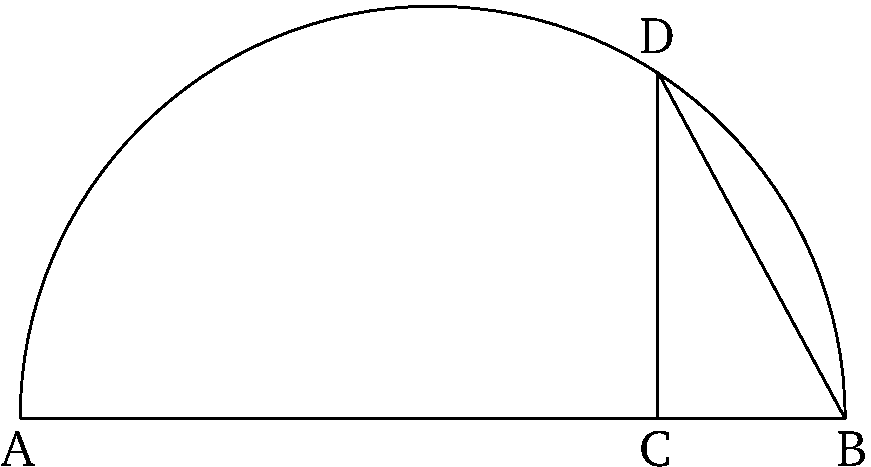
\includegraphics{Book13/fig16ae.pdf}}

Let the diameter $AB$ of the given sphere be laid out, and let it be
cut at $C$ such that $AC$ is four times $CB$ [Prop.~6.10]. And
let the semi-circle $ADB$ be drawn on $AB$. And let the straight-line $CD$ be drawn from $C$ at right-angles to $AB$. And let
$DB$ be joined. And let the circle $EFGHK$ be set down,
and let its radius be equal to $DB$.  And let the equilateral and
equiangular pentagon $EFGHK$ be inscribed in circle
$EFGHK$ [Prop.~4.11]. And let the circumferences $EF$, $FG$,
$GH$, $HK$, and $KE$ be cut in half at points $L$, $M$,
$N$, $O$, and $P$ (respectively). And let $LM$, $MN$, $NO$,
$OP$, $PL$, and $EP$ be joined. Thus, pentagon $LMNOP$
is also equilateral, and $EP$ (is) the side of the decagon (inscribed in the circle).
And let the straight-lines $EQ$, $FR$, $GS$, $HT$, and $KU$, which
are equal to the radius of circle $EFGHK$,  have
been set up at right-angles to the plane of the circle, at points $E$, $F$, $G$, $H$, and $K$ (respectively). And let $QR$, $RS$, $ST$, $TU$,
$UQ$, $QL$, $LR$, $RM$, $MS$, $SN$, $NT$, $TO$,
$OU$, $UP$, and $PQ$ be joined.

And since $EQ$ and $KU$ are each at right-angles to the same plane, $EQ$ is thus parallel to $KU$ [Prop.~11.6]. And it is also equal to it. And straight-lines joining equal and parallel (straight-lines) on the same side are
(themselves) equal and parallel [Prop.~1.33]. Thus, $QU$
is equal and parallel to $EK$. And $EK$ (is the side) of an equilateral
pentagon (inscribed in circle $EFGHK$). Thus, $QU$ (is) also  the
side of an equilateral pentagon inscribed in circle $EFGHK$.  So, for the
same (reasons), $QR$, $RS$, $ST$, and $TU$ are also  the sides of
an equilateral pentagon inscribed in circle $EFGHK$. Pentagon
$QRSTU$ (is) thus equilateral. And side $QE$
is (the side) of a hexagon (inscribed in circle $EFGHK$),
and $EP$ (the side) of a decagon, and (angle) $QEP$ is a right-angle, 
thus $QP$ is  (the side) of a pentagon (inscribed in the same circle).
For the square on the side of a pentagon is (equal to the sum of)
the (squares) on (the sides of) a hexagon and a decagon inscribed in the
same circle  [Prop.~13.10]. So, for the same (reasons), $PU$
is also the side of a pentagon. And $QU$ is also (the
side) of a pentagon. Thus, triangle $QPU$ is equilateral. So, for the
same (reasons), (triangles) $QLR$, $RMS$, $SNT$, and $TOU$
are each also equilateral. And since $QL$ and $QP$ were each shown
(to be the sides) of a pentagon,  and $LP$ is  also (the side) of a pentagon, triangle $QLP$ is thus equilateral. So,
for the same (reasons), triangles $LRM$, $MSN$, $NTO$, and
$OUP$ are each also equilateral. 

% Removed epsf size command
\centerline{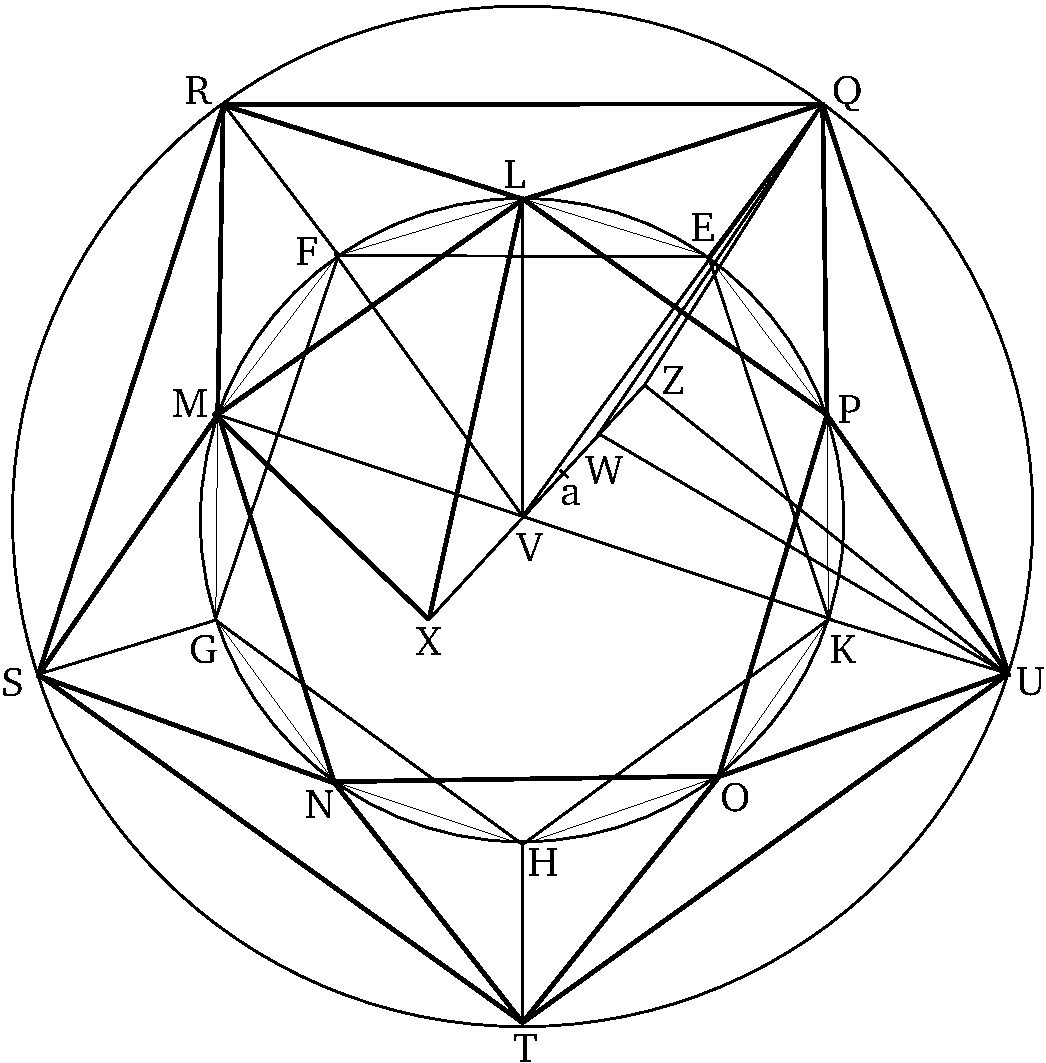
\includegraphics{Book13/fig16e.pdf}}

Let the center, point $V$, of circle $EFGHK$ be found [Prop.~3.1]. 
And let $VZ$ be set up, at (point) $V$,  at right-angles to the plane of the
circle. And let it be produced on the other side (of the circle), 
like $VX$. And let $VW$ be cut off 
(from $XZ$ so as to be equal to the side) of a hexagon, and each of $VX$ and 
$WZ$ (so as to be equal to the side) of a decagon. And let
$QZ$,  $QW$, $UZ$, $EV$, $LV$, $LX$, and
$XM$ be joined.

And since $VW$ and $QE$ are each at right-angles to the plane of the
circle, $VW$ is thus parallel to $QE$ [Prop.~11.6].  And they are also
equal. $EV$ and $QW$ are thus equal and parallel (to one another) [Prop.~1.33]. And $EV$ (is the side) of a hexagon. Thus, $QW$
(is) also (the side) of a hexagon. And since $QW$ is (the side) of a hexagon, 
and $WZ$ (the side) of a decagon, and angle $QWZ$ is a right-angle
[Def.~11.3, Prop.~1.29], 
$QZ$ is thus (the side) of a pentagon [Prop.~13.10]. So, for the same
(reasons), $UZ$ is also (the side) of a pentagon---inasmuch as, if we join
$VK$ and $WU$ then they will be equal and opposite. 
And $VK$, being (equal)
to the radius (of the circle), is (the side) of a hexagon [Prop.~4.15~corr.].
Thus, $WU$ (is) also the side of a hexagon.
 And $WZ$
(is the side) of a decagon, and (angle) $UWZ$ (is) a right-angle. 
Thus, $UZ$ (is the side) of a pentagon [Prop.~13.10]. And $QU$ is
also (the side) of a pentagon. Triangle $QUZ$ is thus equilateral. So,
for the same (reasons), each of the remaining triangles, whose bases
are the straight-lines $QR$, $RS$, $ST$, and $TU$, and apexes the point
$Z$, are also equilateral. Again, since $VL$ (is the side) of a hexagon, and $VX$ (the side) of a decagon, and angle $LVX$ is a right-angle, 
$LX$ is thus (the side) of a pentagon [Prop.~13.10]. So, for the same
(reasons), if we join $MV$, which is (the side) of a hexagon, $MX$
is also inferred (to be the side) of a pentagon. And $LM$ is also (the side)
of a pentagon. Thus, triangle $LMX$ is equilateral. So, similarly,
it can be shown that each of the remaining triangles, whose bases
are the (straight-lines) $MN$, $NO$, $OP$, and $PL$, and apexes the
point $X$,  are also equilateral. Thus, an icosahedron contained by
twenty equilateral triangles has been constructed.

So, it is also necessary to enclose it in the given sphere, and to show
that the side of the icosahedron is that irrational (straight-line) called minor.

For, since $VW$ is (the side) of a hexagon, and $WZ$ (the side) of
a decagon, $VZ$ has thus been cut in extreme and mean
ratio at $W$, and $VW$ is its greater piece  [Prop.~13.9]. Thus, as
$ZV$ is to $VW$, so $VW$ (is) to $WZ$. And $VW$ (is) equal
to $VE$, and $WZ$ to $VX$.  Thus, as $ZV$ is to $VE$,
so $EV$ (is) to $VX$. And angles $ZVE$ and
$EVX$ are right-angles. Thus, if we join straight-line $EZ$ then angle
$XEZ$ will be a right-angle, on account of the similarity of triangles
$XEZ$ and $VEZ$.  [Prop.~6.8]. So, for the same (reasons), since
as $ZV$ is to $VW$, so $VW$ (is) to $WZ$,  and $ZV$ (is) equal to
$XW$, and $VW$ to $WQ$, thus as $XW$ is to $WQ$, so $QW$
(is) to $WZ$. And, again, on account of this,  if we join $QX$ then the
angle at $Q$ will be a right-angle [Prop.~6.8]. Thus, the semi-circle
drawn on $XZ$ will also pass through $Q$ [Prop.~3.31]. And if $XZ$ remains
fixed, and the semi-circle is carried around, and again established at
the same (position) from which it began to be moved, then it will
also pass through (point) $Q$, and (through) the remaining (angular) points
of the icosahedron. And the icosahedron will be enclosed by a sphere.
 So, I say that (it is) also (enclosed) by the given (sphere). 
 For let $VW$ be cut in half at $a$. And since the straight-line $VZ$ has been cut in extreme and mean ratio at $W$, and  $ZW$ is its lesser piece,
 then the square on $ZW$ added to half of the greater piece, $Wa$, is
 five times the (square) on half of the greater piece [Prop.~13.3]. 
 Thus, the (square) on $Za$ is five times the (square) on $aW$. And
 $ZX$ is double $Za$, and $VW$ double $aW$. Thus,
 the (square) on $ZX$ is five times the (square) on $WV$. And since
 $AC$ is four times $CB$, $AB$ is thus five times $BC$. And as
 $AB$ (is) to $BC$, so the (square) on $AB$ (is) to the
 (square) on $BD$ [Prop.~6.8, Def.~5.9]. Thus, the (square)
 on $AB$ is five times the (square) on $BD$. And the (square) on 
 $ZX$ was also shown (to be) five times the (square) on $VW$. 
 And $DB$ is equal to $VW$. For each of them is equal to the
 radius of circle $EFGHK$.  Thus, $AB$ (is) also equal to
 $XZ$.  And $AB$ is the diameter of the given sphere. Thus,
 $XZ$ is equal to the diameter of the given sphere. Thus, the icosahedron
 has been enclosed by the given sphere.
 
 So, I say that the side of the icosahedron is that irrational (straight-line)
 called minor. For since the diameter of the sphere is rational, and the
 square on it is five times the (square) on the radius of circle
 $EFGHK$, the radius of circle $EFGHK$ is thus also rational.
 Hence, its diameter is also rational. And if an equilateral
 pentagon is inscribed in a circle having a rational diameter then
 the side of the pentagon is that irrational (straight-line) called minor [Prop.~13.11]. And the side of pentagon $EFGHK$ is (the side)
 of the icosahedron. Thus, the side of the icosahedron is that irrational
 (straight-line) called minor.}
\end{Parallel}

\begin{Parallel}{}{}
\ParallelLText{
\begin{center}
{\large \gr{Πόρισμα}.}
\end{center}\vspace*{-7pt}

\gr{Ἐκ δὴ τούτου φανερόν, <ότι ἡ τῆξ σφαίραξ διάμετροξ δυνάμει
πενταπλασίων ἐστὶ τῆξ ἐκ τοῦ κέντρου τοῦ κύκλου,
ἀφ> ο<ῦ τὸ εἰκοσάεδρον ἀναγέγραπται, καὶ <ότι
ἡ τῆξ σφαίραξ διάμετροξ σύγκειται >έκ τε τῆξ τοῦ
ἑχαγώνου καὶ δύο τῶν τοῦ δεκαγώνου τῶν εἰξ
τὸν α\kern -.7pt  ὐτὸν κύκλον ἐγγραφομένων. <όπερ >έδει
δεῖχαι.}}

\ParallelRText{
\begin{center}
{\large Corollary}
\end{center}

So,  (it is) clear, from this, that the square on the diameter of the sphere
is five times the square on the radius of the circle from which the icosahedron has been described,
and that the the diameter of the sphere is the sum of (the side) of the hexagon, 
and two of (the sides) of the decagon, inscribed in the same circle.$^\dag$ }
\end{Parallel}
{\footnotesize\noindent$^\dag$ If the radius of the sphere is unity then the
radius of the circle is $2/\sqrt{5}$, and the sides of the hexagon, decagon,
and pentagon/icosahedron are $2/\sqrt{5}$, $1-1/\sqrt{5}$, and $(1/\sqrt{5})\,\sqrt{10-2\,\sqrt{5}}$, respectively.}

%%%%
%13.17
%%%%
\pdfbookmark[1]{Proposition 13.17}{pdf13.17}
\begin{Parallel}{}{}
\ParallelLText{
\begin{center}
{\large \ggn{17}.}
\end{center}\vspace*{-7pt}

\gr{Δωδεκάεδρον συστήσασθαι καὶ σφαίρᾳ περιλαβεῖν, <ῆ| καὶ τὰ
προειρημένα σθήματα, καὶ δεῖχαι, <ότι ἡ τοῦ δωδεκαέδρου
πλευρὰ >άλογόξ ἐστιν ἡ καλουμένη ἀποτομ\kern -.7pt  ή.}

\gr{Ἐκκείσθωσαν τοῦ προειρημένου κύβου δύο ἐπίπεδα πρὸξ
ὀρθὰξ ἀλλήλοιξ τὰ ΑΒΓΔ, ΓΒΕΖ, καὶ τετμ\kern -.7pt  ήσθω ἑκάστη τῶν
ΑΒ, ΒΓ, ΓΔ, ΔΑ, ΕΖ, ΕΒ, ΖΓ πλευρῶν δίθα κατὰ τὰ Η, Θ, Κ, Λ, Μ, Ν, Χ,
καὶ ἐπεζεύθθωσαν αἱ ΗΚ, ΘΛ, ΜΘ, ΝΧ, καὶ τετηήσθω ἑκάστη τῶν
ΝΟ, ΟΧ, ΘΠ >άκρον καὶ μέσον λόγον κατὰ τὰ Ρ, Σ, Τ σημεῖα,
καὶ >έστω α\kern -.7pt  ὐτῶν μείζονα τμ\kern -.5pt  ήματα τὰ ΡΟ, ΟΣ, ΤΠ, καὶ ἀνεστάτωσαν
ἀπὸ τῶν Ρ, Σ, Τ σημείων τοῖξ τοῦ κύβου ἐπιπέδοιξ
πρὸξ ὀρθὰξ ἐπὶ τὰ ἐκτὸξ μέρη τοῦ κύβου αἱ ΡΥ, ΣΦ, ΤΘ,
καὶ κείσθωσαν >ίσαι ταῖξ ΡΟ, ΟΣ, ΤΠ, καὶ ἐπεζεύθθωσαν
αἱ ΥΒ, ΒΘ, ΘΓ, ΓΦ, ΦΥ.}\\~\\~\\

% Removed epsf size command
\centerline{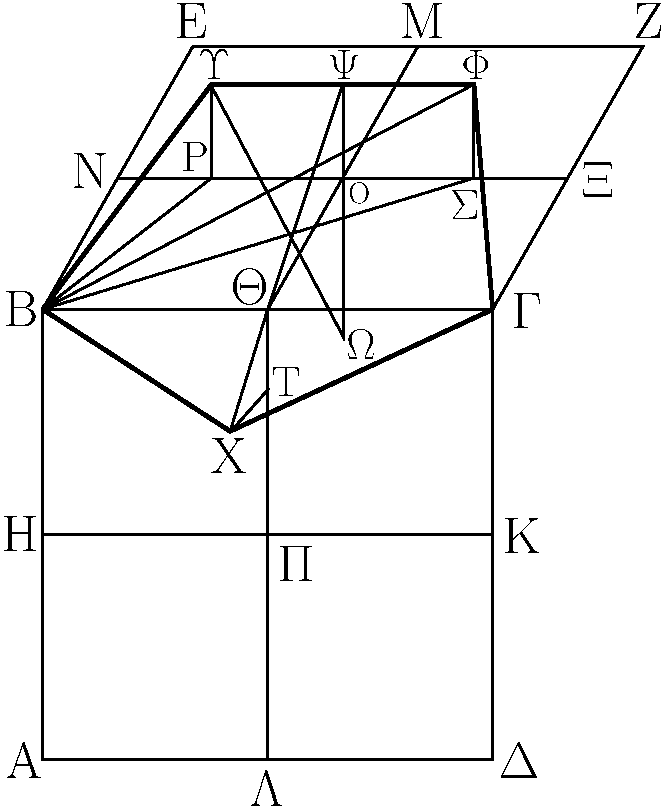
\includegraphics{Book13/fig17g.pdf}}

\gr{Λέγω, <ότι τὸ ΥΒΘΓΦ πεντάγωνον
ἰσόπλευρόν τε καὶ ἐν ἑνὶ ἐπιπέδῳ καὶ >έτι ἰσογώνιόν ἐστιν.
ἐπεζεύθθωσαν γὰρ αἱ ΡΒ, ΣΒ, ΦΒ. καὶ ἐπεὶ εὐθεῖα ἡ ΝΟ >άκρον
καὶ μέσον λόγον τέτμ\kern -.7pt  ηται κατὰ τὸ Ρ, καὶ τὸ μεῖζον τμ\kern -.7pt  ῆμά
ἐστιν ἡ ΡΟ, τὰ >άρα ἀπὸ τῶν ΟΝ, ΝΡ τριπλάσιά ἐστι τοῦ 
ἀπὸ τῆξ ΡΟ. >ίση δὲ ἡ μὲν ΟΝ τῆ| ΝΒ, ἡ δὲ ΟΡ τῆ| ΡΥ; τὰ
>άρα ἀπὸ τῶν ΒΝ, ΝΡ τριπλάσιά ἐστι τοῦ ἀπὸ τῆξ ΡΥ.
τοῖξ δὲ ἀπὸ τῶν ΒΝ, ΝΡ τὸ ἀπὸ τῆξ ΒΡ ἐστιν
>ίσον; τὸ >άρα ἀπὸ τῆξ ΒΡ τριπλάσιόν ἐστι τοῦ ἀπὸ τῆξ ΡΥ;
<ώστε τὰ ἀπὸ τῶν ΒΡ, ΡΥ τετραπλάσιά ἐστι τοῦ ἀπὸ τῆξ ΡΥ.
τοῖξ δὲ ἀπὸ τῶν ΒΡ, ΡΥ >ίσον ἐστι τὸ ἀπὸ τῆξ ΒΥ; τὸ
>άρα >άπὸ τῆξ ΒΥ τετραπλάσιόν ἐστι τοῦ ἀπὸ τῆξ ΥΡ;  διπλῆ >άρα
ἐστὶν ἡ ΒΥ τῆξ ΡΥ. >έστι δὲ καὶ ἡ ΦΥ τῆξ ΥΡ διπλῆ, 
ἐπειδήπερ καὶ ἡ ΣΡ τῆξ ΟΡ, τουτέστι τῆξ ΡΥ, ἐστι διπλῆ;
>ίση >άρα ἡ ΒΥ τῆ| ΥΦ. ὁμοίωξ δὴ δειθθήσεται, <ότι
καὶ ἑκάστη  τῶν ΒΘ, ΘΓ, ΓΦ ἑκατέρᾳ τῶν ΒΥ, ΥΦ
ἐστιν >ίση. ἰσόπλευρον >άρα ἐστὶ τὸ ΒΥΦΓΘ πεντάγωνον. λέγω
δή, <ότι καὶ ἐν ἑνί  ἐστιν ἐπιπέδῳ. >ήθθω γὰρ ἀπὸ τοῦ Ο
ἑκατέρᾳ τῶν ΡΥ, ΣΦ παράλληλοξ ἐπὶ τὰ ἐκτὸξ τοῦ
κύβου μέρη ἡ ΟΨ, καὶ ἐπεζεύθθωσαν αἱ ΨΘ, ΘΘ;
λέγω,  <ότι ἡ ΨΘΘ εὐθεῖά ἐστιν. ἐπεὶ γὰρ ἡ ΘΠ >άκρον καὶ
μέσον λόγον τέτμ\kern -.5pt  ηται κατὰ τὸ Τ, καὶ τὸ μεῖζον α\kern -.3pt  ὐτῆξ
τμ\kern -.7pt  ῆμά ἐστιν ἡ ΠΤ, >έστιν >άρα ὡξ ἡ ΘΠ πρὸξ τὴν 
ΠΤ, ο<ύτωξ ἡ ΠΤ πρὸξ τὴν ΤΘ.  >ίση δὲ ἡ μὲν ΘΠ
τῆ| ΘΟ, ἡ δὲ ΠΤ ἑκατέρᾳ τῶν ΤΘ, ΟΨ; >έστιν >άρα ὡξ
ἡ ΘΟ πρὸξ τὴν ΟΨ, ο<ύτωξ ἡ ΘΤ πρὸξ τὴν ΤΘ. καί ἐστι
παράλληλοξ ἡ μὲν ΘΟ τῆ| ΤΘ; ἑκατέρα γὰρ α\kern -.7pt  ὐτῶν
τῶ| ΒΔ ἐπιπέδῳ πρὸξ ὀρθάξ ἐστιν; ἡ δὲ ΤΘ
τῆ| ΟΨ; ἑκατέρα γὰρ α\kern -.7pt  ὐτῶν τῶ| ΒΖ ἐπιπέδῳ
πρὸξ ὀρθάξ ἐστιν.  ἒαν δὲ δύο τρίγωνα συντεθῆ| κατὰ μίαν
γωνίαν, ὡξ τὰ ΨΟΘ, ΘΤΘ, τὰξ δύο πλευρὰξ ταῖξ δυνὶν ἀνάλογον
>έθοντα, <ώστε τὰξ ὁμολόγουξ α\kern -.7pt  ὐτῶν πλευρὰξ καὶ παραλλήλουξ
ε>ῖναι, αἱ λοιπαὶ εὐθεῖαι ἐπ> εὐθείαξ >έσονται; ἐπ> εὐθείαξ
>άρα ἐστὶν ἡ ΨΘ τῆ| ΘΘ. πᾶσα δὲ εὐθεῖα ἐν ἑνί
ἐστιν ἐπιπέδῳ; ἐν ἑνὶ >άρα ἐπιπέδῳ ἐστὶ τὸ ΥΒΘΓΦ πεντάγωνον.}

\gr{Λέγω δή, <ότι καὶ ἰσογώνιόν ἐστιν.}

\gr{Ἐπεὶ γὰρ εὐθεῖα γραμμ\kern -.7pt  ὴ ἡ ΝΟ >άκρον καὶ μέσον λόγον
τέτμ\kern -.7pt  ηται κατὰ τὸ Ρ, καὶ τὸ μεῖζον τμ\kern -.5pt  ῆμά
ἐστιν ἡ ΟΡ [>έστιν >άρα ὡξ συναμφότεροξ ἡ ΝΟ, ΟΡ πρὸξ
τὴν ΟΝ, ο<ύτωξ ἡ ΝΟ πρὸξ τὴν ΟΡ], >ίση δὲ ἡ ΟΡ
τῆ| ΟΣ [>έστιν >άρα ὡξ ἡ ΣΝ πρὸξ τὴν ΝΟ, ο<ύτωξ
ἡ ΝΟ πρὸξ τὴν ΟΣ], ἡ ΝΣ >άρα >άκρον καὶ μέσον λόγον
τέτμ\kern -.3pt  ηται κατὰ τὸ Ο, καὶ τὸ μεῖζον τμ\kern -.7pt  ῆμά
ἐστιν ἡ ΝΟ; τὰ >άρα ἀπὸ τῶν ΝΣ, ΣΟ τριπλάσιά ἐστι τοῦ ἀπὸ
τῆξ ΝΟ. >ίση δὲ ἡ μὲν ΝΟ τῆ| ΝΒ, ἡ δὲ ΟΣ τῆ| ΣΦ; τὰ
>άρα ἀπὸ τῶν ΝΣ, ΣΦ τετράγωνα τριπλάσιά ἐστι τοῦ ἀπὸ τῆξ
ΝΒ; <ώστε τὰ ἀπὸ τῶν ΦΣ, ΣΝ, ΝΒ τετραπλάσιά ἐστι  τοῦ ἀπὸ
τῆξ ΝΒ. τοῖξ δὲ ἀπὸ τῶν ΣΝ, ΝΒ >ίσον ἐστὶ τὸ ἀπὸ
τῆξ ΣΒ; τὰ >άρα ἀπὸ τῶν ΒΣ, ΣΦ, τουτέστι τὸ ἀπὸ τῆξ
ΒΦ [ὀρθὴ γὰρ ἡ ὑπὸ ΦΣΒ γωνία], τετραπλάσιόν
ἐστι τοῦ ἀπὸ τῆξ ΝΒ; διπλῆ >άρα ἐστὶν ἡ ΦΒ τῆξ ΒΝ.
>έστι δὲ καὶ ἡ ΒΓ τῆξ ΒΝ διπλῆ; >ίση  >άρα ἐστὶν ἡ ΒΦ τῆ| ΒΓ. καὶ
ἐπεὶ δύο αἱ ΒΥ, ΥΦ δυσὶ ταῖξ ΒΘ, ΘΓ >ίσαι εἰσίν, καὶ
βάσιξ ἡ ΒΦ βάσει τῆ| ΒΓ >ίση, γωνία >άρα ἡ ὑπὸ ΒΥΦ
γωνίᾳ τῆ| ὑπὸ ΒΘΓ ἐστιν >ίση. ὁμοίωξ δὴ δείχομεν,
<ότι καὶ ἡ ὑπὸ ΥΦΓ γωνία >ίση ἐστὶ τῆ| ὑπὸ ΒΘΓ;
αἱ >άρα ὑπὸ ΒΘΓ, ΒΥΦ, ΥΦΓ τρεῖξ γωνίαι >ίσαι
ἀλλήλαιξ εἰσίν. ἒαν δὲ πενταγώνου ἰσοπλεύρου αἱ 
τρεῖξ γωνίαι >ίσαι ἀλλήλαιξ >ῶσιν, ἰσογώνιον >έσται
τὸ πεντάγωνον; ἰσογώνιον >άρα ἐστὶ τὸ ΒΥΦΓΘ πεντάγωνον.
ἐδείθθη δὲ καὶ ἰσόπλευρον;
τὸ >άρα ΒΥΦΓΘ πεντάγωνον ἰσόπλευρόν ἐστι καὶ ἰσογώνιον,
καί ἐστιν ἐπὶ μιᾶξ τοῦ κύβου πλευρᾶξ τῆξ ΒΓ. ἒαν
>άρα ἐφ> ἑκάστηξ τῶν τοῦ κύβου δώδεκα
πλευρῶν τὰ α\kern -.7pt  ὐτὰ κατασκευάσωμεν, συσταθήσεταί τι σθῆμα
στερεὸν ὑπὸ δώδεκα πενταγώνων ἰσοπλεύρων
τε καὶ ἰσογωνίων περιεχόμενον, <ὸ καλεῖται δωδεκάεδρον.}

\gr{Δεῖ δὴ α\kern -.7pt  ὐτὸ καὶ σφαίρᾳ περιλαβεῖν τῆ| δοθείσῃ καὶ δεῖχαι,
<ότι ἡ τοῦ δωδεκαέδρου πλευρὰ >άλογόξ ἐστιν ἡ καλουμένη 
ἀποτομ\kern -.7pt  ή.}

\gr{Ἐκβεβλήσθω γὰρ ἡ ΨΟ, καὶ >έστω ἡ ΨΩ; συμβάλλει >άρα
ἡ ΟΩ τῆ| τοῦ κύβου διαμέτρῳ, καὶ δίθα
τέμνουσιν ἀλλήλαξ; τοῦτο γὰρ δέδεικται ἐν τῶ|
παρατελεύτῳ θεωρήματι  τοῦ ἑνδεκάτου βιβλίου. τεμνέτωσαν
κατὰ τὸ Ω; τὸ Ω >άρα κέντρον ἐστὶ τῆξ σφαίραξ τῆξ περιλαμβανούσηξ
τὸν κύβον,
καὶ ἡ ΩΟ ἡμίσεια τῆξ πλευρᾶξ τοῦ κύβου.
 ἐπεζεύθθω δὴ ἡ ΥΩ. καὶ ἐπεὶ εὐθεῖα γραμμ\kern -.7pt  ὴ ἡ ΝΣ
>άκρον καὶ μέσον λόγον τέτμ\kern -.7pt  ηται κατὰ τὸ Ο, καὶ
τὸ μεῖζον α\kern -.5pt  ὐτῆξ τμ\kern -.3pt  ῆμά ἐστιν ἡ ΝΟ, τὰ >άρα ἀπὸ τῶν ΝΣ, ΣΟ
τριπλάσιά ἐστι τοῦ ἀπὸ τῆξ ΝΟ. >ίση δὲ ἡ μὲν ΝΣ τῆ| ΨΩ,
ἐπειδήπερ καὶ ἡ μὲν ΝΟ τῆ| ΟΩ ἐστιν >ίση, ἡ δὲ ΨΟ τῆ|
ΟΣ. ἀλλὰ μ\kern -.7pt  ὴν
καὶ ἡ ΟΣ τῆ| ΨΥ, ἐπεὶ καὶ τῆ| ΡΟ; τὰ >άρα ἀπὸ τῶν
 ΩΨ, ΨΥ τριπλάσιά ἐστι τοῦ ἀπὸ τῆξ ΝΟ. τοῖξ
δὲ ἀπὸ τῶν ΩΨ, ΨΥ >ίσον ἐστὶ τὸ ἀπὸ τῆξ ΥΩ; τὸ
>άρα ἀπὸ τῆξ ΥΩ τριπλάσιόν ἐστι τοῦ ἀπὸ τῆξ ΝΟ.
>έστι δὲ καὶ ἡ ἐκ τοῦ κέντρου τῆξ σφαίραξ τῆξ περιλαμβανούσηξ
τὸν κύβον δυνάμει τριπλασίων τῆξ ἡμισείαξ
τῆξ τοῦ κύβου πλευρᾶξ; προδέδεικται γὰρ κύβον συστήσασθαι
καὶ σφαίρᾳ περιλαβεῖν καὶ δεῖχαι, <ότι ἡ τῆξ σφαίραξ
διάμετροξ δυνάμει τριπλασίων ἐστὶ τῆξ πλευρᾶξ τοῦ κύβου.
εἰ δὲ <όλη τῆξ <όληξ, καὶ [ἡ] ἡμίσεια τῆξ ἡμισείαξ; καί ἐστιν
ἡ ΝΟ ἡμίσεια τῆξ
τοῦ κύβου πλευρᾶξ; ἡ >άρα
ΥΩ >ίση ἐστὶ τῆ| ἐκ τοῦ κέντρου τῆξ σφαίραξ τῆξ περιλαμβανούσηξ
τὸν κύβον. καί ἐστι τὸ Ω κέντρον τῆξ σφαίραξ τῆξ περιλαμβανούσηξ
τὸν κύβον; τὸ Υ >άρα σημεῖον πρὸξ τῆ| ἐπιφανείᾳ ἐστι τῆξ
σφαίραξ. ὁμοίωξ δὴ δείχομεν, <ότι καὶ 
ἑκάστη τῶν λοιπῶν γωνιῶν τοῦ δωδεκαέδρου πρὸξ τῆ|
ἐπιφανείᾳ ἐστὶ τῆξ
σφαίραξ; περιείληπται >άρα τὸ δωδεκαέδρον τῆ| δοθείσῃ σφαίρᾳ.}

\gr{Λέγω δή, <ότι ἡ τοῦ δωδεκαέδρου πλευρὰ >άλογόξ
ἐστιν ἡ καλουμένη ἀποτομ\kern -.7pt  ή.}

\gr{Ἐπεὶ γὰρ τῆξ ΝΟ >άκρον καὶ μέσον λόγον τετμ\kern -.7pt  ημένηξ τὸ
μεῖζον τμ\kern -.7pt  ῆμά ἐστιν ὁ ΡΟ, τῆξ δὲ ΟΧ >άκρον καὶ μέσον
λόγον τετμ\kern -.5pt  ημένηξ τὸ μεῖζον τμ\kern -.3pt  ῆμά ἐστιν ἡ ΟΣ, <όληξ >άρα
τῆξ ΝΧ >άκρον καὶ μέσον λόγον
τεμνομένηξ τὸ μεῖζον τμ\kern -.7pt  ῆμά ἐστιν ἡ ΡΣ. [ο<ῖον ἐπεί
ἐστιν ὡξ ἡ ΝΟ πρὸξ τὴν ΟΡ, ἡ ΟΡ πρὸξ τὴν ΡΝ, καὶ
τὰ διπλάσια; τὰ γὰρ μέρη τοῖξ ἰσάκιξ πολλαπλασίοιξ
τὸν α\kern -.7pt  ὐτὸν >έθει λόγον; ὡξ >άρα ἡ ΝΧ πρὸξ τὴν ΡΣ, ο<ύτωξ
ἡ ΡΣ πρὸξ συναμφότερον τὴν ΝΡ, ΣΧ. μείζων δὲ ἡ ΝΧ
τῆξ ΡΣ; μείζων >άρα καὶ ἡ ΡΣ συναμφοτέρου τῆξ ΝΡ, ΣΧ; ἡ ΝΧ
>άρα >άκρον  καὶ μέσον λόγον τέτμ\kern -.7pt  ηται, καὶ
  τὸ μεῖζον  α\kern -.7pt  ὐτῆξ τμ\kern -.7pt  ῆμά
ἐστιν ἡ ΡΣ.] >ίση δὲ ἡ ΡΣ τῆ| ΥΦ; τῆξ >άρα ΝΧ >άκρον
καὶ μέσον λόγον τεμνομένηξ τὸ μεῖζον τμ\kern -.7pt  ῆμά ἐστιν ἡ
ΥΦ. καὶ ἐπεὶ <ρητή ἐστιν τῆξ σφαίραξ διάμετροξ
καί ἐστι δυνάμει τριπλασίων τῆξ τοῦ κύβου πλευρᾶξ, <ρητὴ
>άρα ἐστὶν ἡ ΝΧ πλευρὰ ο>ῦσα τοῦ κύβου. ἒαν δὲ
<ρητὴ γραμμ\kern -.7pt  ὴ >άκρον καὶ μέσον λόγον τμ\kern -.7pt  ηθῆ|, ἑκάτερον
τῶν τμ\kern -.7pt  ημάτων >άλογόξ ἐστιν ἀποτομ\kern -.7pt  ή.}

\gr{Ἡ ΥΦ >άρα πλευρὰ ο>ῦσα τοῦ δωδεκαέδρου >άλογόξ
ἐστιν ἀποτομ\kern -.7pt  ή.}}

\ParallelRText{
\begin{center}
{\large Proposition 17}
\end{center}

To construct a dodecahedron, and to enclose (it) in a sphere, like the
aforementioned figures, and to show that the side of the dodecahedron 
is that irrational (straight-line) called an apotome.

Let two planes of the aforementioned cube [Prop. 13.15], $ABCD$ and $CBEF$,  (which are) at right-angles to one another,
be laid out. And let the sides $AB$, $BC$, $CD$, $DA$, $EF$,
$EB$, and $FC$  have each been cut in half at points $G$, $H$, $K$, $L$,
$M$, $N$, and $O$ (respectively). And let $GK$, $HL$, $MH$, and
$NO$ be joined. And let $NP$, $PO$, and $HQ$ have each been
cut in extreme and mean ratio at points $R$, $S$, and $T$ (respectively).
And let their greater pieces be $RP$, $PS$, and $TQ$ (respectively).
And let $RU$, $SV$, and $TW$ be set up on the exterior side of the cube,  at points
$R$, $S$, and $T$ (respectively), at right-angles to the planes of the cube.
 And let them be made equal to $RP$,
$PS$, and $TQ$. And let
$UB$, $BW$, $WC$, $CV$, and $VU$ be joined.

% Removed epsf size command
\centerline{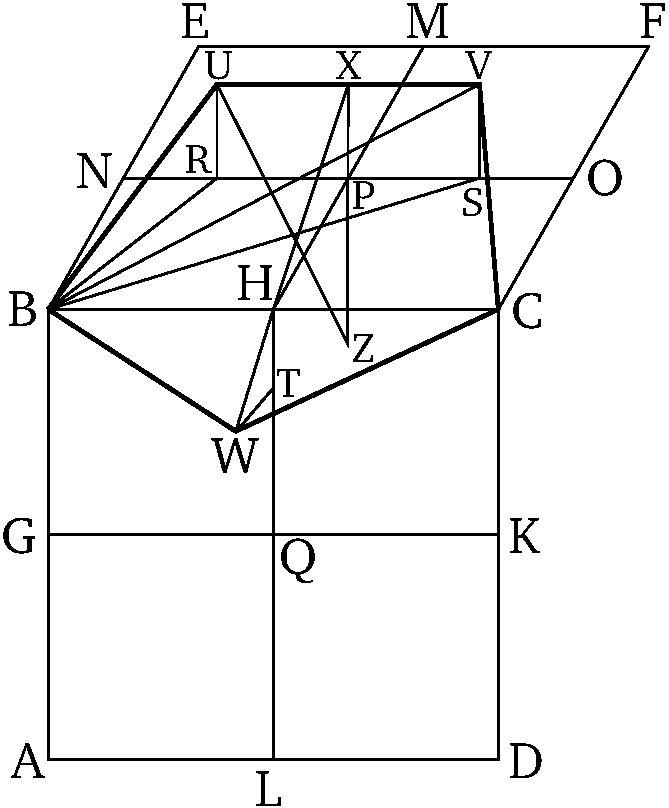
\includegraphics{Book13/fig17e.pdf}}

I say that the pentagon $UBWCV$ is equilateral, and in one plane, and,
further, equiangular. For let $RB$, $SB$, and $VB$ be joined. 
And since the straight-line $NP$ has been cut in extreme and mean
ratio at $R$, and $RP$ is the greater piece,  the (sum of the squares)
on $PN$ and $NR$ is thus three times the (square) on $RP$ [Prop.~13.4].
And $PN$ (is) equal to $NB$, and $PR$ to $RU$. 
Thus, the (sum of the squares) on $BN$ and $NR$ is three times the
(square) on $RU$. And the (square) on $BR$ is equal to the (sum of the squares) on $BN$ and $NR$ [Prop.~1.47].  
Thus, the (square) on $BR$ is three times the (square) on $RU$. 
Hence, the (sum of the
squares) on $BR$ and $RU$ is four times the (square) on $RU$. And
the (square)
on $BU$ is equal to the (sum of the squares) on $BR$ and $RU$ [Prop.~1.47]. Thus, the (square) on $BU$ is four times the
(square) on $UR$.  Thus, $BU$ is double $RU$.  And
$VU$ is also double $UR$, inasmuch as $SR$ is also double $PR$---that is to say, $RU$. Thus, $BU$ (is) equal to $UV$. So, similarly, it can be shown
that  each of $BW$, $WC$, $CV$ is equal to each of $BU$ and $UV$. 
Thus, pentagon $BUVCW$ is equilateral. So, I say that it is also in one plane. For let $PX$ be drawn from $P$, parallel to
each of $RU$ and $SV$, on the exterior side of the cube. And let
$XH$ and $HW$ be joined. I say that $XHW$ is a straight-line.
For since $HQ$ has been cut in extreme and mean ratio at $T$,
and  $QT$  is its greater piece, thus as $HQ$ is to $QT$, so $QT$
(is) to $TH$. And $HQ$ (is) equal to $HP$, and $QT$ to each of
$TW$ and $PX$. Thus, as $HP$ is to $PX$, so $WT$ (is) to
$TH$. And $HP$ is parallel to $TW$. For of each of them is at right-angles
to the plane $BD$ [Prop.~11.6]. And $TH$ (is parallel) to
$PX$. For each of them is at right-angles to the plane $BF$ [Prop.~11.6].
And if two triangles, like
$XPH$ and $HTW$, having two sides proportional to two sides,
are placed together at a single angle  such that their corresponding sides are also parallel then the remaining sides will be straight-on (to one another) [Prop.~6.32]. Thus, $XH$ is straight-on to
$HW$. And every straight-line is in one plane [Prop.~11.1]. Thus,
pentagon $UBWCV$ is in one plane.

So, I say that it is also equiangular.

For since the straight-line $NP$ has been cut in extreme and mean ratio at
$R$, and $PR$ is the greater piece [thus as the sum of
$NP$ and $PR$ is to $PN$, so $NP$ (is) to $PR$], and $PR$
(is) equal to $PS$ [thus as $SN$ is to $NP$, so $NP$ (is) to $PS$], 
$NS$ has thus also been cut in extreme and mean ratio at $P$, and $NP$
is the greater piece [Prop.~13.5]. Thus, the (sum of the squares) on
$NS$ and $SP$ is three times the (square) on $NP$ [Prop.~13.4].
And $NP$ (is) equal to $NB$, and $PS$ to $SV$. Thus, the (sum of the)
squares on  $NS$ and $SV$ is three times the (square) on $NB$.
Hence, the (sum of the squares) on $VS$, $SN$, and $NB$
is four times the (square) on $NB$. And the (square) on $SB$
is equal to the (sum of the squares) on
$SN$ and $NB$  [Prop.~1.47].
Thus, the (sum of the squares) on $BS$ and $SV$---that is to say, 
the (square) on $BV$ [for angle $VSB$ (is) a right-angle]---is
four times the (square) on $NB$ [Def.~11.3, Prop.~1.47].
Thus, $VB$ is double $BN$. And $BC$ (is) also double $BN$.
Thus, $BV$ is equal to $BC$. And since the two (straight-lines)
$BU$ and $UV$ are equal to the two (straight-lines)
$BW$ and $WC$ (respectively), and the base $BV$ (is) equal to
the base $BC$, angle $BUV$ is thus equal to angle $BWC$ [Prop.~1.8].
So, similarly, we can show that angle $UVC$ is equal to angle
$BWC$.  Thus, the three angles
$BWC$, $BUV$, and $UVC$ are equal to one another.
And if three angles of an equilateral pentagon are equal to one another
then the pentagon is equiangular [Prop.~13.7].  Thus, pentagon
$BUVCW$ is equiangular. And it was also shown (to be)
equilateral. Thus, pentagon $BUVCW$ is equilateral and equiangular,
and it is on one of the sides, $BC$, of the cube. Thus, if we make the
same construction on each of the twelve sides of the cube then some solid
figure contained by twelve equilateral and equiangular pentagons 
will be constructed,  which is called a dodecahedron.

So, it is necessary to enclose it in the given sphere, and to show that the
side of the dodecahedron is that irrational (straight-line) called an apotome.

For let $XP$ be produced, and let (the produced straight-line) be $XZ$. Thus, $PZ$ meets
the diameter of the cube, and they cut one another in half.
For, this has been proved in the penultimate theorem of the eleventh book [Prop.~11.38]. Let them cut (one another) at $Z$. Thus, $Z$ is the
center of the sphere enclosing the cube, and $ZP$ (is) half the side of
the cube. So, let $UZ$ be joined. And since the straight-line 
$NS$ has been cut in extreme and mean ratio at $P$, and its greater piece
is $NP$, the (sum of the squares) on $NS$ and $SP$
is thus three times the (square) on $NP$ [Prop.~13.4]. And $NS$ (is)
equal to $XZ$, inasmuch as $NP$ is also equal to $PZ$, and
$XP$ to $PS$. But, indeed, $PS$ (is) also (equal) to $XU$,
since (it is) also (equal) to $RP$. Thus, the (sum of the squares) on 
$ZX$ and $XU$ is three times the (square) on $NP$.
And  the (square)
on $UZ$ is equal to the (sum of the squares) on $ZX$ and $XU$ [Prop.~1.47].  Thus, the (square) on $UZ$ is three times the
(square) on $NP$. 
 And the square on the
radius of the sphere enclosing the cube is also three times the (square) on half
the side of the cube. For it has previously been demonstrated (how to) construct 
the cube, and to enclose (it) in a sphere, and to show that the square on
the diameter of the sphere is three times the (square) on the
side of the cube [Prop.~13.15]. And if the (square on the) whole (is three
times) the (square on the) whole, then the (square on the) half (is) also (three times) the (square on the) half. 
And $NP$ is half of the side of the cube. Thus, $UZ$ is equal to
the radius of the sphere enclosing the cube. And $Z$ is the center of the
sphere enclosing the cube.
Thus, point $U$
is on the surface of the sphere. So, similarly, we can show that each of
the remaining angles of the dodecahedron is also  on the surface of the sphere. 
Thus, the dodecahedron has been enclosed by the given sphere.

So, I say that the side of the dodecahedron is that irrational straight-line
called an apotome.

For since  $RP$ is the greater piece of $NP$, which has been cut in extreme and mean ratio, and $PS$ is the greater piece of $PO$, which
has been cut in extreme and mean ratio,  $RS$ is thus the greater piece of the
whole of $NO$, which has been cut in extreme and mean ratio.
[Thus, since as $NP$ is to $PR$, (so) $PR$ (is) to $RN$, and  (the same is also true) of the doubles.
For parts have the same ratio as similar multiples (taken in corresponding
order) [Prop.~5.15]. Thus, as $NO$ (is) to $RS$, so $RS$
(is) to the sum of $NR$ and $SO$. And $NO$
(is) greater than $RS$. Thus, $RS$ (is) also
greater than the sum of $NR$ and $SO$ [Prop.~5.14]. Thus, $NO$
has been cut in extreme and mean ratio, and  $RS$ is its greater piece.]
And $RS$ (is) equal to $UV$. Thus, $UV$ is the greater piece of
$NO$, which has been cut in extreme and mean ratio. 
And since the diameter of the sphere is rational, and the square on it
is three times the (square) on the side of the cube,  $NO$, which is
the side of the cube, is thus rational. And if a rational (straight)-line
is cut in extreme and mean ratio then each of the
pieces is the irrational (straight-line called) an apotome.

Thus, $UV$, which is the side of the dodecahedron, is the
irrational (straight-line called) an apotome [Prop. 13.6].
}
\end{Parallel}

\begin{Parallel}{}{}
\ParallelLText{
\begin{center}
{\large \gr{Πόρισμα}.}
\end{center}\vspace*{-7pt}

\gr{Ἐκ δὴ τούτου φανερόν, <ότι τῆξ τοῦ κύβου πλευρᾶξ
>άκρον καὶ μέσον λόγον τεμνομένηξ τὸ μεῖζον
τμ\kern -.7pt  ῆμά ἐστιν ἡ τοῦ δωδεκαέδρου πλευρά. <όπερ
>έδει δεῖχαι.}}

\ParallelRText{
\begin{center}
{\large Corollary}
\end{center}

So, (it is) clear, from this, that the side of the dodecahedron
is the greater piece of the side of the cube, when it is cut in extreme
and mean ratio.$^\dag$ (Which is) the very thing it was required to show.}
\end{Parallel}
{\footnotesize\noindent$^\dag$ If the radius of the circumscribed sphere is
unity then the side of the cube is $\sqrt{4/3}$, and the side of the
dodecahedron is $(1/3)\,(\sqrt{15}-\sqrt{3})$.}

%%%%
%13.18
%%%%
\pdfbookmark[1]{Proposition 13.18}{pdf13.18}
\begin{Parallel}{}{}
\ParallelLText{
\begin{center}
{\large \ggn{18}.}
\end{center}\vspace*{-7pt}

\gr{Τὰξ πλευρὰξ τῶν πέντε σθημάτων ἐκθέσθαι καὶ
συγκρῖν\-αι πρὸξ ἀλλήλαξ.}

% Removed epsf size command
\centerline{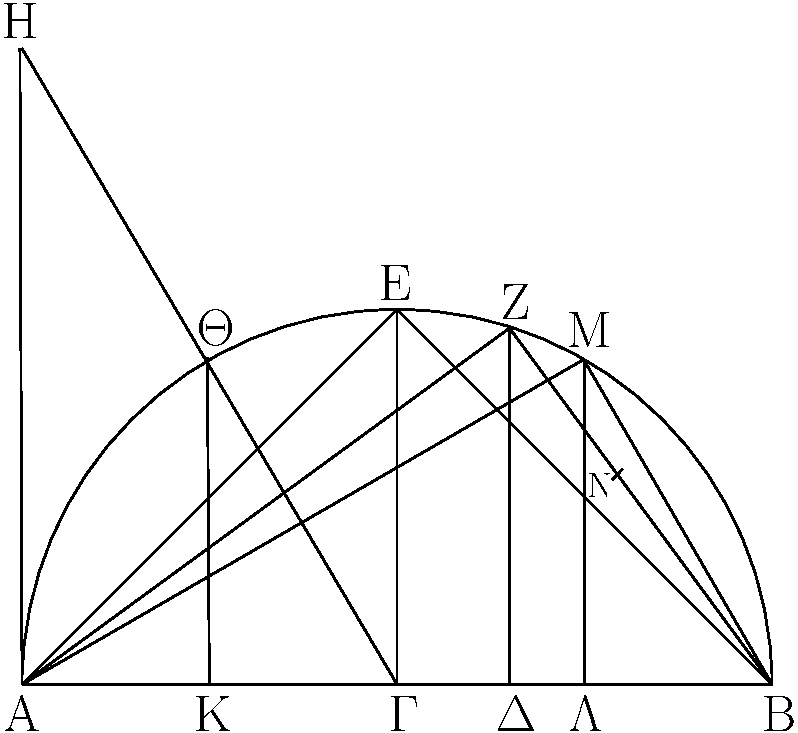
\includegraphics{Book13/fig18g.pdf}}

\gr{Ἐκκείσθω ἡ τῆξ δοθείσηξ σφαίραξ διάμετροξ ἡ ΑΒ, καὶ
τετμ\kern -.7pt  ήσθω κατὰ τὸ Γ <ώστε >ίσην ε>ῖναι τὴν ΑΓ τῆ| ΓΒ, κατὰ
δὲ τὸ Δ <ώστε διπλασίονα ε>ῖναι τὴν ΑΔ τῆξ ΔΒ, καὶ
γεγράφθω ἐπὶ τῆξ ΑΒ ἡμικύκλιον τὸ ΑΕΒ, καὶ ἀπὸ τῶν
Γ, Δ τῆ| ΑΒ πρὸξ ὀρθὰξ >ήθθωσαν αἱ ΓΕ, ΔΖ, καὶ ἐπεζεύθθωσαν
αἱ ΑΖ, ΖΒ, ΕΒ. καὶ ἐπεὶ διπλῆ ἐστιν ἡ ΑΔ τῆξ ΔΒ,
τριπλῆ >άρα ἐστὶν ἡ ΑΒ τῆξ ΒΔ. ἀναστρέψαντι ἡμιολία
>άρα ἐστὶν ἡ ΒΑ τῆξ ΑΔ. ὡξ δὲ ἡ ΒΑ πρὸξ τὴν ΑΔ,
ο<ύτωξ τὸ ἀπὸ τῆξ ΒΑ πρὸξ τὸ ἀπὸ τῆξ ΑΖ;
ἰσογώνιον γάρ ἐστι τὸ ΑΖΒ τρίγωνον τῶ| ΑΖΔ
τριγώνῳ; ἡμιόλιον >άρα ἐστὶ τὸ ἀπὸ τῆξ ΒΑ τοῦ ἀπὸ
τῆξ ΑΖ. >έστι δὲ καὶ ἡ τῆξ σφαίραξ διάμετροξ δυνάμει
ἡμιολία τῆξ πλευρᾶξ τῆξ πυραμίδοξ. καί ἐστιν ἡ ΑΒ
ἡ τῆξ σφαίραξ διάμετροξ; ἡ ΑΖ >άρα >ίση ἐστὶ τῆ|
πλευρᾶ| τῆξ πυραμίδοξ.}

\gr{Πάλιν, ἐπεὶ διπλασίων ἐστὶν ἡ ΑΔ τῆξ ΔΒ, τριπλῆ
>άρα ἐστὶν ἡ ΑΒ τῆξ ΒΔ. ὡξ δὲ ἡ ΑΒ πρὸξ τὴν ΒΔ,
ο<ύτωξ τὸ ἀπὸ τῆξ ΑΒ πρὸξ τὸ ἀπὸ τῆξ ΒΖ; τριπλάσιον
>άρα ἐστὶ τὸ ἀπὸ τῆξ ΑΒ τοῦ ἀπὸ τῆξ ΒΖ. >έστι
δὲ καὶ ἡ τῆξ σφαίραξ διάμετροξ δυνάμει τριπλασίων
τῆξ τοῦ κύβου πλευρᾶξ. καί ἐστιν ἡ ΑΒ ἡ τῆξ σφαίραξ
διάμετροξ; ἡ ΒΖ >άρα τοῦ κύβου ἐστὶ πλευρά.}

\gr{Καὶ ἐπεὶ >ίση ἐστὶν ἡ ΑΓ τῆ| ΓΒ, διπλῆ >άρα
ἐστὶν ἡ ΑΒ τῆξ ΒΓ. ὡξ δὲ ἡ ΑΒ πρὸξ τὴν ΒΓ, ο<ύτωξ
τὸ ἀπὸ τῆξ ΑΒ πρὸξ τὸ ἀπὸ τῆξ ΒΕ; διπλάσιον
>άρα ἐστὶ τὸ ἀπὸ τῆξ ΑΒ τοῦ ἀπὸ τῆξ ΒΕ. >έστι
δὲ καὶ ἡ τῆξ σφαίραξ διάμετροξ δυνάμει διπλασίων
τῆξ τοῦ ὀκταέδρου πλευρᾶξ. καὶ ἐστιν ἡ ΑΒ ἡ
τῆξ δοθείσηξ σφαίραξ διάμετροξ; ἡ ΒΕ >άρα τοῦ ὀκταέδρου
ἐστὶ πλευρά.}

\gr{>'Ηθθω δὴ ἀπὸ τοῦ Α σημείου τῆ| ΑΒ εὐθείᾳ
πρὸξ ὀρθὰξ ἡ ΑΗ, καὶ κείσθω ἡ ΑΗ >ίση τῆ| ΑΒ,
καὶ ἐπεζεύθθω ἡ ΗΓ, καὶ ἀπὸ τοῦ Θ ἐπὶ
τὴν ΑΒ κάθετοξ >ήθθω ἡ ΘΚ. καὶ ἐπεὶ διπλῆ ἐστιν
ἡ ΗΑ τῆξ ΑΓ; >ίση γὰρ ἡ ΗΑ τῆ| ΑΒ; ὡξ δὲ ἡ ΗΑ
πρὸξ τὴν ΑΓ, ο<ύτωξ ἡ ΘΚ πρὸξ τὴν ΚΓ, διπλῆ >άρα
καὶ ἡ ΘΚ τῆξ ΚΓ. τετραπλάσιον >άρα ἐστὶ τὸ ἀπὸ
τῆξ ΘΚ τοῦ ἀπὸ τῆξ ΚΓ; τὰ >άρα ἀπὸ τῶν ΘΚ, ΚΓ,
<όπερ ἐστὶ τὸ ἀπὸ τῆξ ΘΓ, πενταπλάσιόν  ἐστι τοῦ
ἀπὸ τῆξ ΚΓ. >ίση δὲ ἡ ΘΓ τῆ| ΓΒ; πενταπλάσιον
>άρα ἐστὶ τὸ ἀπὸ τῆξ ΒΓ τοῦ ἀπὸ τῆξ ΓΚ. καὶ
ἐπεὶ διπλῆ ἐστιν ἡ ΑΒ τῆξ ΓΒ, <ῶν ἡ ΑΔ τῆξ
ΔΒ ἐστι διπλῆ,  λοιπὴ >άρα ἡ ΒΔ λοιπῆξ τῆξ ΔΓ ἐστι
διπλῆ. τριπλῆ >άρα ἡ ΒΓ τῆξ ΓΔ; ἐνναπλάσιον >άρα τὸ
ἀπὸ τῆξ ΒΓ τοῦ ἀπὸ τῆξ ΓΔ. πενταπλάσιον δὲ τὸ ἀπὸ
τῆξ ΒΓ τοῦ ἀπὸ τῆξ ΓΚ; μεῖζον >άρα τὸ ἀπὸ τῆξ
ΓΚ τοῦ ἀπὸ τῆξ ΓΔ. μείζων >άρα ἐστὶν ἡ ΓΚ τῆξ
ΓΔ. κείσθω τῆ| ΓΚ >ίση ἡ ΓΛ, καὶ ἀπὸ τοῦ Λ τῆ|
ΑΒ πρὸξ ὀρθὰξ >ήθθω ἡ ΛΜ, καὶ ἐπεζεύθθω ἡ ΜΒ.
καὶ ἐπεὶ πενταπλάσιόν ἐστι τὸ ἀπὸ  τῆξ ΒΓ τοῦ ἀπὸ τῆξ
ΓΚ, καί ἐστι τῆξ μὲν ΒΓ διπλῆ ἡ ΑΒ, τῆξ δὲ ΓΚ διπλῆ
ἡ ΚΛ, πενταπλάσιον >άρα ἐστὶ τὸ ἀπὸ τῆξ ΑΒ τοῦ ἀπὸ τῆξ
ΚΛ.
>έστι δὲ καὶ ἡ τῆξ σφαίραξ διάμετροξ δυνάμει πενταπλασίων
τῆξ ἐκ τοῦ κέντρου τοῦ κύκλου, ἀφ> ο<ῦ τὸ εἰκοσάεδρον
ἀναγέγραπται. καί ἐστιν ἡ ΑΒ ἡ τῆξ σφαίραξ διάμετροξ;
ἡ ΚΛ >άρα ἐκ τοῦ κέντρου ἐστὶ τοῦ κύκλου, ἀφ> ο<ῦ
τὸ εἰκοσάεδρον ἀναγέγραπται; ἡ ΚΛ >άρα ἑχαγώνου ἐστὶ
πλευρὰ τοῦ εἰρημένου κύκλου. καὶ ἐπεὶ ἡ τῆξ σφαίραξ
διάμετροξ σύγκειται >έκ τε τῆξ τοῦ ἑχαγώνου καὶ δύο τῶν
τοῦ δεκαγώνου τῶν εἰξ τὸν εἰρημένον κύκλον ἐγγραφομένων,
καί ἐστιν ἡ μὲν ΑΒ ἡ τῆξ σφαίραξ διάμετροξ, ἡ δὲ ΚΛ
ἑχαγώνου πλευρά, καὶ >ίση ἡ ΑΚ τῆ| ΛΒ, ἑκατέρα >άρα τῶν
ΑΚ, ΛΒ δεκαγώνου ἐστὶ πλευρὰ τοῦ ἐγγραφομένου εἰξ
τὸν κύκλον, ἀφ> ο<ῦ τὸ εἰκοσάεδρον ἀναγέγραπται. καὶ
ἐπεὶ δεκαγώνου μὲν ἡ ΛΒ, ἑχαγώνου δὲ ἡ ΜΛ;
>ίση γάρ ἐστι τῆ| ΚΛ, ἐπεὶ καὶ τῆ| ΘΚ; >ίσον γὰρ ἀπέθουσιν
ἀπὸ τοῦ κέντρου; καί ἐστιν ἑκατέρα τῶν ΘΚ, ΚΛ διπλασίων
τῆξ ΚΓ; πενταγώνου >άρα ἐστὶν ἡ ΜΒ. ἡ δὲ τοῦ πενταγώνου
ἐστὶν ἡ τοῦ εἰκοσαέδρου; εἰκοσαέδρου >άρα ἐστὶν ἡ ΜΒ.}

\gr{Καὶ ἐπεὶ ἡ ΖΒ κύβου ἐστὶ πλευρά, τετμ\kern -.7pt  ήσθω >άκρον καὶ
μέσον λόγον κατὰ τὸ Ν, καὶ >έστω μεῖζον τμ\kern -.7pt  ῆμα τὸ
ΝΒ; ἡ ΝΒ >άρα δωδεκαέδρου ἐστὶ πλευρά.}

\gr{Καὶ ἐπεὶ ἡ τῆξ σφαίραξ διάμετροξ ἐδείθθη τῆξ μὲν
ΑΖ πλευρᾶξ τῆξ πυραμίδοξ δυνάμει ἡμιολία, τῆξ δὲ
τοῦ ὀκταέδρου τῆξ ΒΕ δυνάμει διπλασίων, τῆξ δὲ τοῦ
κύβου τῆξ ΖΒ δυνάμει τριπλασίων, ο<ίων >άρα ἡ τῆξ
σφαίραξ διάμετροξ δυνάμει <έχ, τοιούτων ἡ μὲν τῆξ
πυραμίδοξ τεσσάρων, ἡ δὲ τοῦ ὀκταέδρου τριῶν, ἡ δὲ
τοῦ κύβου δύο.  ἡ μὲν >άρα τῆξ πυραμίδοξ πλευρὰ
τῆξ μὲν τοῦ ὀκταέδρου πλευρᾶξ δυνάμει ἐστὶν ἐπίτριτοξ,
τῆξ δὲ τοῦ κύβου δυνάμει διπλῆ, ἡ δὲ τοῦ ὀκταέδρου τῆξ
τοῦ κύβου δυνάμει ἡμιολία. αἱ μὲν ο>ῦν εἰρημέναι
τῶν τριῶν σθημάτων πλευραί, λέγω δὴ πυραμίδοξ καὶ ὀκταέδρου
καὶ κύβου, πρὸξ ἀλλήλαξ εἰσὶν ἐν λόγοιξ <ρητοῖξ. αἱ δὲ λοιπαὶ
δύο, λέγω δὴ <ή τε τοῦ εἰκοσαέδρου καὶ ἡ τοῦ δωδεκαέδρου,
ο>ύτε πρὸξ ἀλλήλαξ ο>ύτε πρὸξ τὰξ προειρημέναξ εἰσὶν ἐν λόγοιξ
<ρητοῖξ; >άλογοι γάρ εἰσιν, ἡ μὲν ἐλάττων, ἡ δὲ ἀποτομ\kern -.7pt  ή.}

\gr{<'Οτι μείζων ἐστὶν ἡ τοῦ εἰκοσαέδρου πλευρὰ ἡ ΜΒ
τῆξ τοῦ δωδεκαέδρου τῆξ ΝΒ, δείχομεν ο<ύτωξ.}

\gr{Ἐπεὶ γὰρ ἰσογώνιόν ἐστι τὸ ΖΔΒ τρίγωνον τῶ|
ΖΑΒ τριγώνῳ, ἀνάλογόν ἐστιν ὡξ ἡ ΔΒ πρὸξ
τὴν ΒΖ, ο<ύτωξ ἡ ΒΖ πρὸξ τὴν ΒΑ. καὶ ἐπεὶ τρεῖξ
εὐθεῖαι ἀνάλογόν εἰσιν, >έστιν ὡξ ἡ πρώτη πρὸξ
τὴν τρίτην, ο<ύτωξ τὸ ἀπὸ τῆξ πρώτηξ πρὸξ τὸ ἀπὸ
τῆξ δευτέραξ;  >έστιν >άρα ὡξ ἡ ΔΒ πρὸξ τὴν ΒΑ, ο<ύτωξ
τὸ ἀπὸ τῆξ ΔΒ πρὸξ τὸ ἀπὸ τῆξ ΒΖ; ἀνάπαλιν >άρα ὡξ ἡ ΑΒ
πρὸξ τὴν ΒΔ, ο<ύτωξ τὸ ἀπὸ τῆξ ΖΒ πρὸξ τὸ ἀπὸ
τῆξ ΒΔ. τριπλῆ δὲ ἡ ΑΒ τῆξ ΒΔ; τριπλάσιον
>άρα τὸ ἀπὸ τῆξ ΖΒ τοῦ ἀπὸ τῆξ ΒΔ. >έστι
δὲ καὶ τὸ ἀπὸ τῆξ ΑΔ τοῦ ἀπὸ τῆξ ΔΒ τετραπλάσιον;
διπλῆ γὰρ ἡ ΑΔ τῆξ ΔΒ; μεῖζον >άρα τὸ ἀπὸ τῆξ
ΑΔ τοῦ ἀπὸ τῆξ ΖΒ; μείζων >άρα ἡ ΑΔ τῆξ ΖΒ;
πολλῶ| >άρα ἡ ΑΛ τῆξ ΖΒ μείζων ἐστίν. καὶ τῆξ
μὲν ΑΛ >άκρον καὶ μέσον λόγον τεμνομένηξ τὸ μεῖζον
τμ\kern -.7pt  ῆμά ἐστιν ἡ ΚΛ, ἐπειδήπερ ἡ μὲν ΛΚ ἑχαγώνου ἐστίν,
ἡ δὲ ΚΑ δεκαγώνου; τῆξ δὲ ΖΒ >άκρον καὶ μέσον
λόγον τεμνομένηξ τὸ μεῖζον τμ\kern -.7pt  ῆμά ἐστιν ἡ ΝΒ; μείζων
>άρα ἡ ΚΛ τῆξ ΝΒ. >ίση δὲ ἡ ΚΛ τῆ| ΛΜ; μείζων
>άρα ἡ ΛΜ τῆξ ΝΒ [τῆξ δὲ ΛΜ μείζων ἐστὶν ἡ ΜΒ].
πολλῶ| >άρα ἡ ΜΒ πλευρὰ ο>ῦσα τοῦ εἰκοσαέδρου μείζων
ἐστὶ τῆξ ΝΒ πλευρᾶξ ο>ύσηξ τοῦ δωδεκαέδρου; <όπερ
>έδει δεῖχαι.}}

\ParallelRText{
\begin{center}
{\large Proposition 18}
\end{center}

To set out the sides of the five (aforementioned) figures, and to compare (them)
with one another.$^\dag$

% Removed epsf size command
\centerline{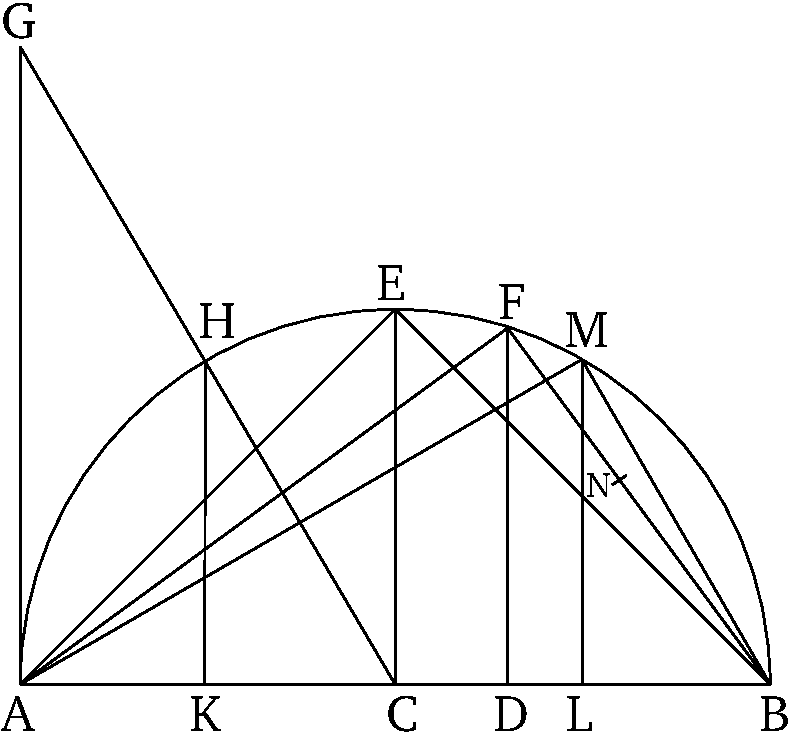
\includegraphics{Book13/fig18e.pdf}}

Let the diameter, $AB$, of the given sphere be laid out. And let it
be cut at $C$, such that $AC$ is equal to $CB$, and at $D$, such
that $AD$ is double $DB$. And let the semi-circle $AEB$ be
drawn on $AB$. And let $CE$ and $DF$ be drawn from $C$
and $D$ (respectively), at right-angles to $AB$. And let $AF$, $FB$,
and $EB$ be joined. And since $AD$ is double $DB$, 
$AB$ is thus triple $BD$. Thus, via conversion, $BA$ is one and
a half times $AD$. And as $BA$ (is) to $AD$, so the (square)
on $BA$ (is) to the (square) on $AF$ [Def.~5.9].  For
triangle $AFB$ is equiangular to triangle $AFD$ [Prop.~6.8]. 
Thus, the (square) on $BA$ is one and a half times the (square)
on $AF$. And the square on the diameter of the sphere
is also one and a half times the (square) on the side of the pyramid
[Prop.~13.13].  And $AB$ is the diameter of the sphere. Thus,
$AF$ is equal to the side of the pyramid.

Again, since $AD$ is double $DB$,  $AB$ is thus triple $BD$. And
as $AB$ (is) to $BD$, so the (square) on $AB$ (is) to the (square)
on $BF$ [Prop.~6.8, Def.~5.9]. Thus, the (square) on $AB$
is three times the (square) on $BF$.  And the square on the diameter of
the sphere is also three times the (square) on the side of the cube [Prop.~13.15]. And $AB$ is the diameter of the sphere. Thus, $BF$ is the
side of the cube.

And since $AC$ is equal to $CB$, $AB$ is thus double $BC$.  And
as $AB$ (is) to $BC$, so the (square) on $AB$ (is) to the (square)
on $BE$ [Prop.~6.8, Def.~5.9]. Thus, the (square) on $AB$
is double the (square) on $BE$. And the square on the diameter
of the sphere is also double the (square) on the side of the octagon [Prop.~13.14]. And $AB$ is the diameter of the given sphere. Thus,
$BE$ is the side of the octagon.

So let $AG$ be drawn from point $A$ at right-angles to the straight-line
$AB$. And let $AG$ be made equal to $AB$. And let $GC$
be joined. And let $HK$ be drawn from $H$, perpendicular to $AB$. And since $GA$ is double $AC$. 
For $GA$ (is) equal to $AB$.  And as $GA$ (is) to $AC$, so
$HK$ (is) to $KC$ [Prop.~6.4]. $HK$ (is) thus also double
$KC$. Thus, the (square) on $HK$ is four times the (square)
on $KC$. Thus, the (sum of the squares) on $HK$ and $KC$,
which is the (square) on $HC$ [Prop.~1.47],  is five times the
(square) on $KC$.  And $HC$ (is) equal to $CB$. Thus,
the (square) on $BC$ (is) five times the (square) on  $CK$. 
And since $AB$ is double $CB$, of which $AD$ is double $DB$, 
the remainder $BD$ is thus double the remainder $DC$.
$BC$ (is) thus triple $CD$. The (square) on $BC$ (is) thus nine times 
the (square) on $CD$.  And the (square) on $BC$ (is) five times the (square)
on $CK$.  Thus, the (square) on $CK$ (is) greater than the (square) on $CD$.
$CK$ is thus greater than $CD$. Let $CL$ be made equal to $CK$.
And let $LM$ be drawn from $L$ at right-angles to $AB$. 
And let $MB$ be joined. And since the (square) on  $BC$
is five times the (square) on $CK$, and $AB$ is double $BC$, and $KL$
double $CK$, the (square) on $AB$ is thus five times the (square)
on $KL$. And the square on the diameter of the sphere  is also five times
the (square) on the radius of the circle from which the icosahedron has been
described [Prop.~13.16~corr.]. And $AB$ is the diameter of the sphere.
Thus, $KL$ is the radius of the circle from which the icosahedron has
been described. Thus, $KL$ is (the side) of the hexagon (inscribed) in the aforementioned
circle [Prop.~4.15~corr.]. And since the diameter of the sphere is composed of (the side) of the hexagon, and two of (the sides) of the decagon, inscribed
in the aforementioned circle, and $AB$ is the diameter of the sphere, 
and $KL$ the side of the hexagon, and $AK$ (is) equal to $LB$, thus
$AK$ and $LB$ are each sides of the decagon inscribed in the  circle
from which the icosahedron has been described. And since
$LB$ is (the side) of the decagon. And $ML$ (is the side) of the hexagon---for (it is) equal to $KL$, since (it is) also (equal) to $HK$, for they are equally
far from the center. And $HK$ and $KL$ are each double $KC$. 
$MB$ is thus (the side) of the pentagon (inscribed in the circle) [Props.~13.10, 1.47]. 
And (the side) of the pentagon is (the side) of the icosahedron [Prop.~13.16]. 
Thus, $MB$ is (the side) of the icosahedron. 

And since $FB$ is the side of the cube, let it be cut in extreme and
mean ratio at $N$, and let $NB$ be the greater piece. Thus, $NB$
is the side of the dodecahedron [Prop.~13.17~corr.].

And since the (square) on the diameter of the sphere was shown (to be)
one and a half times the square on the side, $AF$,  of the pyramid,
and twice the square on (the side), $BE$,  of the octagon, and
three times the square on (the side), $FB$, of the cube, 
thus, of whatever (parts) the (square) on the diameter of the
sphere (makes) six, of such (parts) the (square) on (the side) of the pyramid (makes)
four, and (the square) on (the side) of the octagon three, and (the
square) on (the side) of the cube  two. Thus, the (square) on the
side of the pyramid is one and a third times the square on the side of the
octagon, and double the square on (the side) of the cube. 
And the (square) on (the side) of the octahedron is one and a half
times the square on (the side) of the cube. Therefore, the aforementioned
sides of the three figures---I mean, of the pyramid, and of the octahedron, and 
of the cube---are
in rational ratios to one another. And (the sides of) the remaining two (figures)---I mean, of
the icosahedron, and of the dodecahedron---are neither in rational ratios to
one another, nor to the (sides) of the aforementioned (three figures). For they are
irrational (straight-lines): (namely), a minor [Prop.~13.16], and 
an apotome [Prop.~13.17].

(And), we can show that the side, $MB$, of the icosahedron is greater
that the (side), $NB$, or the dodecahedron, as follows.

For, since triangle $FDB$ is equiangular to triangle $FAB$ [Prop.~6.8],
proportionally, as $DB$ is to $BF$, so $BF$ (is) to $BA$ [Prop.~6.4]. 
And since three straight-lines are (continually) proportional, as the
first (is) to the third, so the (square) on the first (is) to the (square) on the
second [Def.~5.9, Prop.~6.20~corr.]. Thus, as $DB$ is to $BA$, so the (square) on $DB$
(is) to the (square) on $BF$. Thus, inversely, as $AB$ (is) to $BD$, so the
(square) on $FB$ (is) to the (square) on $BD$. And $AB$ (is) triple
$BD$. Thus, the (square) on $FB$ (is) three times the (square)
on $BD$. And the (square) on $AD$ is also four times the (square)
on $DB$. For $AD$ (is) double $DB$. Thus, the (square) on $AD$
(is) greater than the (square) on $FB$.  Thus, $AD$ (is) greater than
$FB$. 
Thus, $AL$ is much greater than $FB$. And $KL$ is the greater piece of $AL$, which is cut in extreme and
mean ratio---inasmuch as $LK$ is (the side) of the hexagon, and $KA$
(the side) of the decagon [Prop.~13.9]. And $NB$
is the greater piece of $FB$, which is cut in extreme and mean ratio. 
Thus, $KL$ (is) greater than $NB$.  And $KL$ (is) equal to $LM$. 
Thus, $LM$ (is) greater than $NB$ [and $MB$ is greater than $LM$].
Thus, $MB$, which is (the side) of the icosahedron, is much greater
than $NB$, which is (the side) of the dodecahedron.  (Which is)
the very thing it was required to show.}
\end{Parallel}
{\footnotesize\noindent$\dag$ If the radius of the given sphere is unity 
then the sides of the pyramid ({\em i.e.}, tetrahedron), octahedron, cube,
icosahedron, and dodecahedron, respectively, satisfy the following
inequality: $\sqrt{8/3} > \sqrt{2}>\sqrt{4/3}>(1/\sqrt{5})\,\sqrt{10 -2\,\sqrt{5}}
> (1/3)\,(\sqrt{15}-\sqrt{3})$.}

\begin{Parallel}{}{}
\ParallelLText{~\\

\gr{Λέγω δή, <ότι παρὰ τὰ εἰρημένα πέντε σθήματα
οὐ συσταθήσεται <έτερον σθῆμα περιεχόμενον ὑπὸ
ἰσοπλεύρων τε καὶ ἰσογωνίων >ίσων ἀλλήλοιξ.}

\gr{Ὑπὸ μὲν γὰρ δύο τριγώνων >ὴ <όλωξ ἐπιπέδων
στερεὰ γωνία οὐ συνίσταται. ὑπὸ δὲ τριῶν τριγώνων
ἡ τῆξ πυραμίδοξ, ὑπὸ δὲ τεσσάρων ἡ τοῦ ὀκταέδρου,
ὑπὸ δὲ πέντε ἡ τοῦ εἰκοσαέδρου; ὑπὸ δὲ <ὲχ τριγώνων
ἰσοπλεύρων τε καὶ ἰσογωνίων πρὸξ ἑνὶ σημείῳ
συνισταμένων οὐκ >έσται στερεὰ γωνία; ο>ύσηξ γὰρ τῆξ
τοῦ ἰσοπλεύρου τριγώνου γωνίαξ διμοίρου ὀρθῆξ
>έσονται αἱ <ὲχ τέσσαρσιν ὀρθαῖξ >ίσαι; <όπερ ἀδύνατον;
<άπασα γὰρ στερεὰ γωνία ὑπὸ ἐλασσόνων >ὴ τεσσάρων
ὀρθῶν περέθεται. διὰ τὰ α\kern -.7pt  ὐτὰ δὴ οὐδὲ ὑπὸ
πλειόνων >ὴ <ὲχ γωνιῶν ἐπιπέδων στερεὰ γωνία
συνίσταται. ὑπὸ δὲ τετραγώνων τριῶν ἡ τοῦ κύβου
γωνία περιέθεται; ὑπὸ δὲ τεσσάρων ἀδύνατον; >έσονται
γὰρ πάλιν τέσσαρεξ ὀρθαί. ὑπὸ δὲ πενταγώνων ἰσοπλεύρων
καὶ ἰσογωνίων, ὑπὸ μὲν τριῶν ἡ τοῦ δωδεκαέδρου;
ὑπὸ δὲ τεσσάρων ἀδύνατον; ο>ύσηξ γὰρ τῆξ τοῦ
πενταγώνου ἰσοπλεύρου γωνίαξ ὀρθῆξ καὶ πέμπτου,
>έσονται αἱ τέσσαρεξ γωνίαι τεσσάρων ὀρθῶν μείζουξ;
<όπερ ἀδύνατον. οὐδὲ μ\kern -.7pt  ὴν ὑπὸ πολυγώνων ἑτέρων
σθημάτων περισθεθήσεται στερεὰ γωνία διὰ τὸ α\kern -.5pt  ὐτὸ
>άτοπον.}

\gr{Οὐκ >άρα παρὰ τὰ εἰρημένα πέντε σθήματα <έτερον
σθῆμα στερεὸν συσταθήσεται ὑπὸ ἰσοπλεύρων
τε καὶ ἰσογωνίων περιεχόμενον; <όπερ
>έδει δεῖχαι.}}

\ParallelRText{~\\

So, I say that, beside the five aforementioned  figures,  no other (solid) figure
can be constructed (which is) contained by equilateral and equiangular (planes), equal to one another.

For a solid angle cannot be constructed from two triangles, or indeed (two) planes (of any sort) [Def.~11.11]. And (the solid angle) of the
pyramid (is constructed) from three (equiangular) triangles, and (that) of the octahedron
from four (triangles), and (that) of the icosahedron from (five) triangles. 
And a solid angle cannot be (made) from six equilateral and
equiangular triangles set up together at one point. For, since the angles of a
equilateral triangle are (each)  two-thirds of a right-angle, the (sum of the)
six  (plane) angles (containing the solid angle) will be four right-angles. The very thing (is) impossible.
For every solid angle is contained by (plane angles whose sum is) less than four right-angles [Prop.~11.21].  So, for the same (reasons), a solid angle cannot be constructed from more than six  plane angles (equal to two-thirds of a right-angle) either. And the (solid) angle of a cube
is contained by three squares. And (a solid angle contained) by four
(squares is) impossible. For, again, the (sum of the plane angles
containing the solid angle) will be four right-angles. And (the solid angle)
of a dodecahedron (is contained) by three equilateral and equiangular
pentagons. And (a solid angle contained) by four (equiangular
pentagons is) impossible. For, the angle of an equilateral
pentagon being one and one-fifth of right-angle, four (such) angles will be
greater (in sum) than four right-angles. The very thing (is) impossible. And, on account of the same absurdity, a solid angle cannot be constructed from any other
(equiangular) polygonal figures either.

Thus, beside the five aforementioned figures, no other solid figure can be constructed (which is) contained by equilateral and equiangular (planes).
(Which is) the very thing it was required to show.}
\end{Parallel}

\begin{Parallel}{}{}
\ParallelLText{

% Removed epsf size command
\centerline{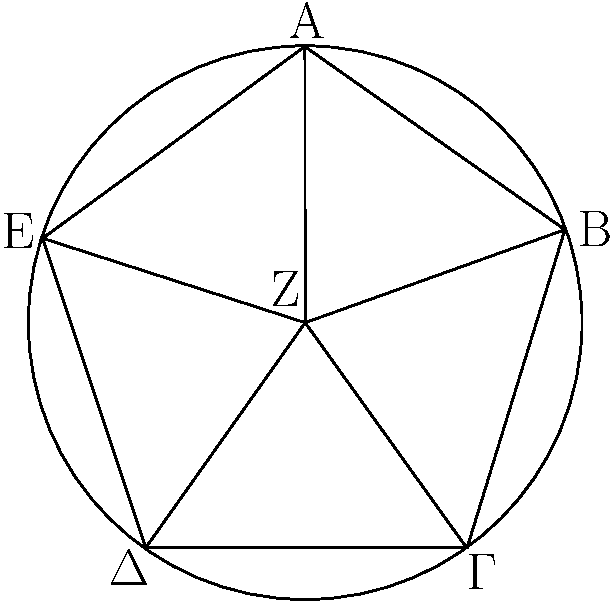
\includegraphics{Book13/fig18ag.pdf}}

\begin{center}\vspace*{-7pt}
{\large \gr{Λῆμμα}.}
\end{center}\vspace*{-7pt}

\gr{<'Οτι δὲ ἡ τοῦ ἰσοπλεύρου καὶ ἰσογωνίου πενταγώνου
γωνία ὀρθή ἐστι καὶ πέμπτου, ο<ύτω δεικτέον.}

\gr{>'Εστω γὰρ πεντάγωνον ἰσόπλευρον καὶ ἰσογώνιον
τὸ ΑΒΓΔΕ, καὶ περιγεγράφθω περὶ α\kern -.7pt  ὐτὸ κύκλοξ ὁ ΑΒΓΔΕ,
καὶ εἰλήφθω α\kern -.7pt  ὐτοῦ τὸ κέντρον τὸ Ζ, καὶ ἐπεζεύθθωσαν
αἱ ΖΑ, ΖΒ, ΖΓ, ΖΔ, ΖΕ. δίθα >άρα τέμνουσι τὰξ πρὸξ τοῖξ
Α, Β, Γ, Δ, Ε τοῦ πενταγώνου γωνίαξ. καὶ ἐπεὶ αἱ πρὸξ
τῶ| Ζ πέντε γωνίαι τέσσαρσιν ὀρθαῖξ >ίσαι εἰσὶ καί
εἰσιν >ίσαι, μία >άρα α\kern -.5pt  ὐτῶν, ὡξ ἡ ὑπὸ ΑΖΒ, μιᾶξ
ὀρθῆξ ἐστι παρὰ πέμπτον; λοιπαὶ >άρα αἱ ὑπὸ ΖΑΒ, ΑΒΖ
μιᾶξ εἰσιν ὀρθῆξ καὶ πέμπτου. >ίση δὲ ἡ ὑπὸ ΖΑΒ τῆ|
ὑπὸ ΖΒΓ; καὶ <όλη >άρα ἡ ὑπὸ ΑΒΓ τοῦ πενταγώνου
γωνία μιᾶξ
ἐστιν  ὀρθῆξ καὶ πέμπτου; <όπερ >έδει δεῖχαι.}}

\ParallelRText{

% Removed epsf size command
\centerline{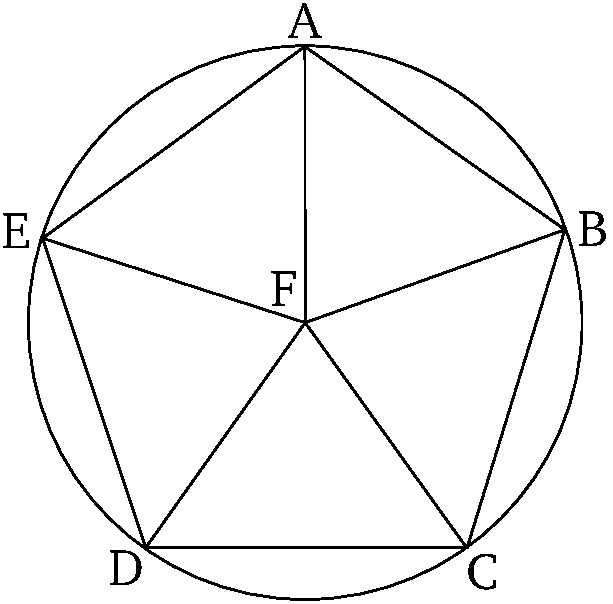
\includegraphics{Book13/fig18ae.pdf}}

\begin{center}\vspace*{-7pt}
{\large Lemma}
\end{center}\vspace*{-7pt}

It can be shown that the angle of an equilateral and
equiangular pentagon is one and one-fifth of a right-angle,
as follows.

For let $ABCDE$ be an equilateral and equiangular pentagon, and
let the circle $ABCDE$ be circumscribed about it [Prop.~4.14]. 
And let its center, $F$, be found [Prop.~3.1]. 
And let $FA$, $FB$, $FC$, $FD$, and $FE$ be joined. Thus,
they cut the angles of the pentagon in half at (points)
 $A$, $B$, $C$, $D$, and $E$  [Prop.~1.4].
 And since the five
angles at $F$ are equal (in sum) to four right-angles, and
are also equal (to one another),  (any) one of them, like $AFB$, is thus
one less a fifth of a right-angle. Thus, the (sum of the) remaining
(angles in triangle $ABF$), $FAB$ and $ABF$,  is one plus a fifth  of a right-angle
[Prop.~1.32]. And $FAB$ (is) equal to $FBC$. Thus, the
whole angle, $ABC$, of the pentagon is also one and one-fifth
of a right-angle. (Which is) the very thing it was required to show.}
\end{Parallel}
